\documentclass[a4paper,11pt,titlepage,oneside,openright]{book}
\usepackage{epsfig} % use eps images
\usepackage{plain} % page numbers always bottom-centered
\usepackage{setspace} % line spacing
\usepackage[paperheight=29.7cm,paperwidth=21cm,outer=1.5cm,inner=2.5cm,top=2cm,bottom=2cm]{geometry} % page layout
\usepackage{titlesec} % custom chapter titles
\usepackage{tocloft} % table of contents with dots
\usepackage{amssymb} % R symbol
\usepackage{amsthm} % theorems
\usepackage{amsmath} % piece-wise function
\usepackage{algorithm} % algorithm
\usepackage[noend]{algpseudocode} % algorithm pseudocode
\usepackage{bm} % bold in formulae
\usepackage{mathabx} % math symbols
\usepackage[utf8x]{inputenc} % special characters support
\usepackage[english]{babel} % english ty­po­graph­i­cal rules, hy­phen­ation, etc
\usepackage[linktocpage=true]{hyperref} % links in TOC
\usepackage{graphicx} % images
\usepackage{subcaption} % images
\usepackage{tabularx} % tables
\usepackage{color}

\renewcommand{\cftchapleader}{\cftdotfill{\cftdotsep}} % TOC dots for chapters
\renewcommand{\cftsecleader}{\cftdotfill{\cftdotsep}} % TOC dots for sections

\newcommand{\todo}[3]{\textcolor{#1}{#2 [{\bf #3}]}}
\newcommand{\todor}[2]{\todo{red}{#1}{#2}}
\newcommand{\todog}[2]{\todo{blue}{#1}{#2}}

\graphicspath{ {./figures/} {../src/out/plots/} }

\newtheorem{Theorem}{Theorem}
\newtheorem{Definition}{Definition}
\newtheorem{Problem}{Problem}

%%%%% NEW MATH DEFINITIONS %%%%%

\newlength{\notationgap}
\setlength{\notationgap}{1pc}

% Mark sections of captions for referring to divisions of figures
\newcommand{\figleft}{{\em (Left)}}
\newcommand{\figcenter}{{\em (Center)}}
\newcommand{\figright}{{\em (Right)}}
\newcommand{\figtop}{{\em (Top)}}
\newcommand{\figbottom}{{\em (Bottom)}}
\newcommand{\captiona}{{\em (a)}}
\newcommand{\captionb}{{\em (b)}}
\newcommand{\captionc}{{\em (c)}}
\newcommand{\captiond}{{\em (d)}}

% Highlight a newly defined term
\newcommand{\newterm}[1]{{\bf #1}}


% Figure reference, lower-case.
\def\figref#1{figure~\ref{#1}}
% Figure reference, capital. For start of sentence
\def\Figref#1{Figure~\ref{#1}}
\def\twofigref#1#2{figures \ref{#1} and \ref{#2}}
\def\quadfigref#1#2#3#4{figures \ref{#1}, \ref{#2}, \ref{#3} and \ref{#4}}
% Section reference, lower-case.
\def\secref#1{section~\ref{#1}}
% Section reference, capital.
\def\Secref#1{Section~\ref{#1}}
% Reference to two sections.
\def\twosecrefs#1#2{sections \ref{#1} and \ref{#2}}
% Reference to three sections.
\def\secrefs#1#2#3{sections \ref{#1}, \ref{#2} and \ref{#3}}
% Reference to an equation, lower-case.
\def\eqref#1{\ref{#1}}
% Reference to an equation, upper case
\def\Eqref#1{\ref{#1}}
% A raw reference to an equation---avoid using if possible
\def\plaineqref#1{\ref{#1}}
% Reference to a chapter, lower-case.
\def\chapref#1{chapter~\ref{#1}}
% Reference to an equation, upper case.
\def\Chapref#1{Chapter~\ref{#1}}
% Reference to a range of chapters
\def\rangechapref#1#2{chapters\ref{#1}--\ref{#2}}
% Reference to an algorithm, lower-case.
\def\algref#1{algorithm~\ref{#1}}
% Reference to an algorithm, upper case.
\def\Algref#1{Algorithm~\ref{#1}}
\def\twoalgref#1#2{algorithms \ref{#1} and \ref{#2}}
\def\Twoalgref#1#2{Algorithms \ref{#1} and \ref{#2}}
% Reference to a part, lower case
\def\partref#1{part~\ref{#1}}
% Reference to a part, upper case
\def\Partref#1{Part~\ref{#1}}
\def\twopartref#1#2{parts \ref{#1} and \ref{#2}}

\def\ceil#1{\lceil #1 \rceil}
\def\floor#1{\lfloor #1 \rfloor}
\def\1{\bm{1}}
\newcommand{\train}{\mathcal{D}}
\newcommand{\valid}{\mathcal{D_{\mathrm{valid}}}}
\newcommand{\test}{\mathcal{D_{\mathrm{test}}}}

\def\eps{{\epsilon}}


% Random variables
\def\reta{{\textnormal{$\eta$}}}
\def\ra{{\textnormal{a}}}
\def\rb{{\textnormal{b}}}
\def\rc{{\textnormal{c}}}
\def\rd{{\textnormal{d}}}
\def\re{{\textnormal{e}}}
\def\rf{{\textnormal{f}}}
\def\rg{{\textnormal{g}}}
\def\rh{{\textnormal{h}}}
\def\ri{{\textnormal{i}}}
\def\rj{{\textnormal{j}}}
\def\rk{{\textnormal{k}}}
\def\rl{{\textnormal{l}}}
% rm is already a command, just don't name any random variables m
\def\rn{{\textnormal{n}}}
\def\ro{{\textnormal{o}}}
\def\rp{{\textnormal{p}}}
\def\rq{{\textnormal{q}}}
\def\rr{{\textnormal{r}}}
\def\rs{{\textnormal{s}}}
\def\rt{{\textnormal{t}}}
\def\ru{{\textnormal{u}}}
\def\rv{{\textnormal{v}}}
\def\rw{{\textnormal{w}}}
\def\rx{{\textnormal{x}}}
\def\ry{{\textnormal{y}}}
\def\rz{{\textnormal{z}}}

% Random vectors
\def\rvepsilon{{\mathbf{\epsilon}}}
\def\rvtheta{{\mathbf{\theta}}}
\def\rva{{\mathbf{a}}}
\def\rvb{{\mathbf{b}}}
\def\rvc{{\mathbf{c}}}
\def\rvd{{\mathbf{d}}}
\def\rve{{\mathbf{e}}}
\def\rvf{{\mathbf{f}}}
\def\rvg{{\mathbf{g}}}
\def\rvh{{\mathbf{h}}}
\def\rvu{{\mathbf{i}}}
\def\rvj{{\mathbf{j}}}
\def\rvk{{\mathbf{k}}}
\def\rvl{{\mathbf{l}}}
\def\rvm{{\mathbf{m}}}
\def\rvn{{\mathbf{n}}}
\def\rvo{{\mathbf{o}}}
\def\rvp{{\mathbf{p}}}
\def\rvq{{\mathbf{q}}}
\def\rvr{{\mathbf{r}}}
\def\rvs{{\mathbf{s}}}
\def\rvt{{\mathbf{t}}}
\def\rvu{{\mathbf{u}}}
\def\rvv{{\mathbf{v}}}
\def\rvw{{\mathbf{w}}}
\def\rvx{{\mathbf{x}}}
\def\rvy{{\mathbf{y}}}
\def\rvz{{\mathbf{z}}}

% Elements of random vectors
\def\erva{{\textnormal{a}}}
\def\ervb{{\textnormal{b}}}
\def\ervc{{\textnormal{c}}}
\def\ervd{{\textnormal{d}}}
\def\erve{{\textnormal{e}}}
\def\ervf{{\textnormal{f}}}
\def\ervg{{\textnormal{g}}}
\def\ervh{{\textnormal{h}}}
\def\ervi{{\textnormal{i}}}
\def\ervj{{\textnormal{j}}}
\def\ervk{{\textnormal{k}}}
\def\ervl{{\textnormal{l}}}
\def\ervm{{\textnormal{m}}}
\def\ervn{{\textnormal{n}}}
\def\ervo{{\textnormal{o}}}
\def\ervp{{\textnormal{p}}}
\def\ervq{{\textnormal{q}}}
\def\ervr{{\textnormal{r}}}
\def\ervs{{\textnormal{s}}}
\def\ervt{{\textnormal{t}}}
\def\ervu{{\textnormal{u}}}
\def\ervv{{\textnormal{v}}}
\def\ervw{{\textnormal{w}}}
\def\ervx{{\textnormal{x}}}
\def\ervy{{\textnormal{y}}}
\def\ervz{{\textnormal{z}}}

% Random matrices
\def\rmA{{\mathbf{A}}}
\def\rmB{{\mathbf{B}}}
\def\rmC{{\mathbf{C}}}
\def\rmD{{\mathbf{D}}}
\def\rmE{{\mathbf{E}}}
\def\rmF{{\mathbf{F}}}
\def\rmG{{\mathbf{G}}}
\def\rmH{{\mathbf{H}}}
\def\rmI{{\mathbf{I}}}
\def\rmJ{{\mathbf{J}}}
\def\rmK{{\mathbf{K}}}
\def\rmL{{\mathbf{L}}}
\def\rmM{{\mathbf{M}}}
\def\rmN{{\mathbf{N}}}
\def\rmO{{\mathbf{O}}}
\def\rmP{{\mathbf{P}}}
\def\rmQ{{\mathbf{Q}}}
\def\rmR{{\mathbf{R}}}
\def\rmS{{\mathbf{S}}}
\def\rmT{{\mathbf{T}}}
\def\rmU{{\mathbf{U}}}
\def\rmV{{\mathbf{V}}}
\def\rmW{{\mathbf{W}}}
\def\rmX{{\mathbf{X}}}
\def\rmY{{\mathbf{Y}}}
\def\rmZ{{\mathbf{Z}}}

% Elements of random matrices
\def\ermA{{\textnormal{A}}}
\def\ermB{{\textnormal{B}}}
\def\ermC{{\textnormal{C}}}
\def\ermD{{\textnormal{D}}}
\def\ermE{{\textnormal{E}}}
\def\ermF{{\textnormal{F}}}
\def\ermG{{\textnormal{G}}}
\def\ermH{{\textnormal{H}}}
\def\ermI{{\textnormal{I}}}
\def\ermJ{{\textnormal{J}}}
\def\ermK{{\textnormal{K}}}
\def\ermL{{\textnormal{L}}}
\def\ermM{{\textnormal{M}}}
\def\ermN{{\textnormal{N}}}
\def\ermO{{\textnormal{O}}}
\def\ermP{{\textnormal{P}}}
\def\ermQ{{\textnormal{Q}}}
\def\ermR{{\textnormal{R}}}
\def\ermS{{\textnormal{S}}}
\def\ermT{{\textnormal{T}}}
\def\ermU{{\textnormal{U}}}
\def\ermV{{\textnormal{V}}}
\def\ermW{{\textnormal{W}}}
\def\ermX{{\textnormal{X}}}
\def\ermY{{\textnormal{Y}}}
\def\ermZ{{\textnormal{Z}}}

% Vectors
\def\vzero{{\bm{0}}}
\def\vone{{\bm{1}}}
\def\vmu{{\bm{\mu}}}
\def\vtheta{{\bm{\theta}}}
\def\va{{\bm{a}}}
\def\vb{{\bm{b}}}
\def\vc{{\bm{c}}}
\def\vd{{\bm{d}}}
\def\ve{{\bm{e}}}
\def\vf{{\bm{f}}}
\def\vg{{\bm{g}}}
\def\vh{{\bm{h}}}
\def\vi{{\bm{i}}}
\def\vj{{\bm{j}}}
\def\vk{{\bm{k}}}
\def\vl{{\bm{l}}}
\def\vm{{\bm{m}}}
\def\vn{{\bm{n}}}
\def\vo{{\bm{o}}}
\def\vp{{\bm{p}}}
\def\vq{{\bm{q}}}
\def\vr{{\bm{r}}}
\def\vs{{\bm{s}}}
\def\vt{{\bm{t}}}
\def\vu{{\bm{u}}}
\def\vv{{\bm{v}}}
\def\vw{{\bm{w}}}
\def\vx{{\bm{x}}}
\def\vy{{\bm{y}}}
\def\vz{{\bm{z}}}

% Elements of vectors
\def\evalpha{{\alpha}}
\def\evbeta{{\beta}}
\def\evepsilon{{\epsilon}}
\def\evlambda{{\lambda}}
\def\evomega{{\omega}}
\def\evmu{{\mu}}
\def\evpsi{{\psi}}
\def\evsigma{{\sigma}}
\def\evtheta{{\theta}}
\def\eva{{a}}
\def\evb{{b}}
\def\evc{{c}}
\def\evd{{d}}
\def\eve{{e}}
\def\evf{{f}}
\def\evg{{g}}
\def\evh{{h}}
\def\evi{{i}}
\def\evj{{j}}
\def\evk{{k}}
\def\evl{{l}}
\def\evm{{m}}
\def\evn{{n}}
\def\evo{{o}}
\def\evp{{p}}
\def\evq{{q}}
\def\evr{{r}}
\def\evs{{s}}
\def\evt{{t}}
\def\evu{{u}}
\def\evv{{v}}
\def\evw{{w}}
\def\evx{{x}}
\def\evy{{y}}
\def\evz{{z}}

% Matrix
\def\mA{{\bm{A}}}
\def\mB{{\bm{B}}}
\def\mC{{\bm{C}}}
\def\mD{{\bm{D}}}
\def\mE{{\bm{E}}}
\def\mF{{\bm{F}}}
\def\mG{{\bm{G}}}
\def\mH{{\bm{H}}}
\def\mI{{\bm{I}}}
\def\mJ{{\bm{J}}}
\def\mK{{\bm{K}}}
\def\mL{{\bm{L}}}
\def\mM{{\bm{M}}}
\def\mN{{\bm{N}}}
\def\mO{{\bm{O}}}
\def\mP{{\bm{P}}}
\def\mQ{{\bm{Q}}}
\def\mR{{\bm{R}}}
\def\mS{{\bm{S}}}
\def\mT{{\bm{T}}}
\def\mU{{\bm{U}}}
\def\mV{{\bm{V}}}
\def\mW{{\bm{W}}}
\def\mX{{\bm{X}}}
\def\mY{{\bm{Y}}}
\def\mZ{{\bm{Z}}}
\def\mBeta{{\bm{\beta}}}
\def\mPhi{{\bm{\Phi}}}
\def\mLambda{{\bm{\Lambda}}}
\def\mSigma{{\bm{\Sigma}}}

% Tensor
\DeclareMathAlphabet{\mathsfit}{\encodingdefault}{\sfdefault}{m}{sl}
\SetMathAlphabet{\mathsfit}{bold}{\encodingdefault}{\sfdefault}{bx}{n}
\newcommand{\tens}[1]{\bm{\mathsfit{#1}}}
\def\tA{{\tens{A}}}
\def\tB{{\tens{B}}}
\def\tC{{\tens{C}}}
\def\tD{{\tens{D}}}
\def\tE{{\tens{E}}}
\def\tF{{\tens{F}}}
\def\tG{{\tens{G}}}
\def\tH{{\tens{H}}}
\def\tI{{\tens{I}}}
\def\tJ{{\tens{J}}}
\def\tK{{\tens{K}}}
\def\tL{{\tens{L}}}
\def\tM{{\tens{M}}}
\def\tN{{\tens{N}}}
\def\tO{{\tens{O}}}
\def\tP{{\tens{P}}}
\def\tQ{{\tens{Q}}}
\def\tR{{\tens{R}}}
\def\tS{{\tens{S}}}
\def\tT{{\tens{T}}}
\def\tU{{\tens{U}}}
\def\tV{{\tens{V}}}
\def\tW{{\tens{W}}}
\def\tX{{\tens{X}}}
\def\tY{{\tens{Y}}}
\def\tZ{{\tens{Z}}}


% Graph
\def\gA{{\mathcal{A}}}
\def\gB{{\mathcal{B}}}
\def\gC{{\mathcal{C}}}
\def\gD{{\mathcal{D}}}
\def\gE{{\mathcal{E}}}
\def\gF{{\mathcal{F}}}
\def\gG{{\mathcal{G}}}
\def\gH{{\mathcal{H}}}
\def\gI{{\mathcal{I}}}
\def\gJ{{\mathcal{J}}}
\def\gK{{\mathcal{K}}}
\def\gL{{\mathcal{L}}}
\def\gM{{\mathcal{M}}}
\def\gN{{\mathcal{N}}}
\def\gO{{\mathcal{O}}}
\def\gP{{\mathcal{P}}}
\def\gQ{{\mathcal{Q}}}
\def\gR{{\mathcal{R}}}
\def\gS{{\mathcal{S}}}
\def\gT{{\mathcal{T}}}
\def\gU{{\mathcal{U}}}
\def\gV{{\mathcal{V}}}
\def\gW{{\mathcal{W}}}
\def\gX{{\mathcal{X}}}
\def\gY{{\mathcal{Y}}}
\def\gZ{{\mathcal{Z}}}

% Sets
\def\sA{{\mathbb{A}}}
\def\sB{{\mathbb{B}}}
\def\sC{{\mathbb{C}}}
\def\sD{{\mathbb{D}}}
% Don't use a set called E, because this would be the same as our symbol
% for expectation.
\def\sF{{\mathbb{F}}}
\def\sG{{\mathbb{G}}}
\def\sH{{\mathbb{H}}}
\def\sI{{\mathbb{I}}}
\def\sJ{{\mathbb{J}}}
\def\sK{{\mathbb{K}}}
\def\sL{{\mathbb{L}}}
\def\sM{{\mathbb{M}}}
\def\sN{{\mathbb{N}}}
\def\sO{{\mathbb{O}}}
\def\sP{{\mathbb{P}}}
\def\sQ{{\mathbb{Q}}}
\def\sR{{\mathbb{R}}}
\def\sS{{\mathbb{S}}}
\def\sT{{\mathbb{T}}}
\def\sU{{\mathbb{U}}}
\def\sV{{\mathbb{V}}}
\def\sW{{\mathbb{W}}}
\def\sX{{\mathbb{X}}}
\def\sY{{\mathbb{Y}}}
\def\sZ{{\mathbb{Z}}}

% Entries of a matrix
\def\emLambda{{\Lambda}}
\def\emA{{A}}
\def\emB{{B}}
\def\emC{{C}}
\def\emD{{D}}
\def\emE{{E}}
\def\emF{{F}}
\def\emG{{G}}
\def\emH{{H}}
\def\emI{{I}}
\def\emJ{{J}}
\def\emK{{K}}
\def\emL{{L}}
\def\emM{{M}}
\def\emN{{N}}
\def\emO{{O}}
\def\emP{{P}}
\def\emQ{{Q}}
\def\emR{{R}}
\def\emS{{S}}
\def\emT{{T}}
\def\emU{{U}}
\def\emV{{V}}
\def\emW{{W}}
\def\emX{{X}}
\def\emY{{Y}}
\def\emZ{{Z}}
\def\emSigma{{\Sigma}}

% entries of a tensor
% Same font as tensor, without \bm wrapper
\newcommand{\etens}[1]{\mathsfit{#1}}
\def\etLambda{{\etens{\Lambda}}}
\def\etA{{\etens{A}}}
\def\etB{{\etens{B}}}
\def\etC{{\etens{C}}}
\def\etD{{\etens{D}}}
\def\etE{{\etens{E}}}
\def\etF{{\etens{F}}}
\def\etG{{\etens{G}}}
\def\etH{{\etens{H}}}
\def\etI{{\etens{I}}}
\def\etJ{{\etens{J}}}
\def\etK{{\etens{K}}}
\def\etL{{\etens{L}}}
\def\etM{{\etens{M}}}
\def\etN{{\etens{N}}}
\def\etO{{\etens{O}}}
\def\etP{{\etens{P}}}
\def\etQ{{\etens{Q}}}
\def\etR{{\etens{R}}}
\def\etS{{\etens{S}}}
\def\etT{{\etens{T}}}
\def\etU{{\etens{U}}}
\def\etV{{\etens{V}}}
\def\etW{{\etens{W}}}
\def\etX{{\etens{X}}}
\def\etY{{\etens{Y}}}
\def\etZ{{\etens{Z}}}

% The true underlying data generating distribution
\newcommand{\pdata}{p_{\rm{data}}}
% The empirical distribution defined by the training set
\newcommand{\ptrain}{\hat{p}_{\rm{data}}}
\newcommand{\Ptrain}{\hat{P}_{\rm{data}}}
% The model distribution
\newcommand{\pmodel}{p_{\rm{model}}}
\newcommand{\Pmodel}{P_{\rm{model}}}
\newcommand{\ptildemodel}{\tilde{p}_{\rm{model}}}
% Stochastic autoencoder distributions
\newcommand{\pencode}{p_{\rm{encoder}}}
\newcommand{\pdecode}{p_{\rm{decoder}}}
\newcommand{\precons}{p_{\rm{reconstruct}}}

\newcommand{\laplace}{\mathrm{Laplace}} % Laplace distribution

\newcommand{\E}{\mathbb{E}}
\newcommand{\Ls}{\mathcal{L}}
\newcommand{\R}{\mathbb{R}}
\newcommand{\emp}{\tilde{p}}
\newcommand{\lr}{\alpha}
\newcommand{\reg}{\lambda}
\newcommand{\rect}{\mathrm{rectifier}}
\newcommand{\softmax}{\mathrm{softmax}}
\newcommand{\sigmoid}{\sigma}
\newcommand{\softplus}{\zeta}
\newcommand{\KL}{D_{\mathrm{KL}}}
\newcommand{\Var}{\mathrm{Var}}
\newcommand{\standarderror}{\mathrm{SE}}
\newcommand{\Cov}{\mathrm{Cov}}
% Wolfram Mathworld says $L^2$ is for function spaces and $\ell^2$ is for vectors
% But then they seem to use $L^2$ for vectors throughout the site, and so does
% wikipedia.
\newcommand{\normlzero}{L^0}
\newcommand{\normlone}{L^1}
\newcommand{\normltwo}{L^2}
\newcommand{\normlp}{L^p}
\newcommand{\normmax}{L^\infty}

\newcommand{\parents}{Pa} % See usage in notation.tex. Chosen to match Daphne's book.

\DeclareMathOperator*{\argmax}{arg\,max}
\DeclareMathOperator*{\argmin}{arg\,min}

\DeclareMathOperator{\sign}{sign}
\DeclareMathOperator{\Tr}{Tr}
\let\ab\allowbreak


\begin{document}
    \singlespacing
    \pagenumbering{gobble} % no page numbering
    \pagestyle{plain}

\thispagestyle{empty}

\begin{center}
    \begin{figure}[h!]
    \centerline{
\psfig{file=logo_unitn_black_center.eps,width=0.6\textwidth}}
    \end{figure}

    \vspace{2 cm}
    \LARGE{Department of Information Engineering and Computer Science\\}

    \vspace{1 cm} 
    \Large{Master's Degree in Computer Science\\}

    \vspace{2 cm} 
    \Large\textsc{Final Dissertation\\}
    
    \vspace{1 cm} 
    \Huge\textsc{Constrained Adversarial Networks\\}

    \vspace{2 cm} 
    \begin{tabular*}{\textwidth}{ c @{\extracolsep{\fill}} c }
    \Large{Supervisor} & \Large{Student}\\
    \Large{Prof. Andrea Passerini}& \Large{Gianvito Taneburgo}\\\\
    \Large{Co-supervisor}\\
    \Large{Dr. Paolo Morettin}\\\\
    \end{tabular*}

    \vspace{2 cm}
    \Large{Academic year 2016/2017}
\end{center}

    \clearpage
    
    \pagestyle{plain}
    \mainmatter % Arabic page numbering

    \tableofcontents
    \clearpage
    \chapter*{List of Acronyms}

\begin{minipage}{\linewidth}
\bgroup
\def\arraystretch{1.5}
\begin{tabularx}{\textwidth}{Xl}
Artificial Intelligence \dotfill & AI\\
Artificial Neural Network \dotfill & ANN\\
Boundary-seeking Generative Adversarial Networks \dotfill & BGANs\\
Constrained Adversarial Networks \dotfill & CANs\\
Constrained Optimization Problem \dotfill & COP\\ 
Central Processing Unit \dotfill & CPU\\
Constraint Satisfaction Problem \dotfill & CSP\\
Deep Learning \dotfill & DL\\
Feedforward Neural Network \dotfill & FNN\\
Generative Adversarial Networks \dotfill & GANs\\
Graphics Processing Unit \dotfill & GPU\\
Machine Learning \dotfill & ML\\
Recurrent Neural Network \dotfill & RNN\\
Propositional Satisfiability Problem \dotfill & SAT
\end{tabularx}
\egroup
\end{minipage}

%     \chapter*{Notation}

\vspace{\notationgap}
% Need to use minipage to keep title of table on same page as table
\begin{minipage}{\textwidth}
% This is a hack to put a little title over the table
% We cannot use "\section*", etc., they appear in the table of contents.
% tocdepth does not work on this chapter.
\centerline{\bf Numbers and Arrays}
\bgroup
% The \arraystretch definition here increases the space between rows in the table,
% so that \displaystyle math has more vertical space.
\def\arraystretch{1.5}
\begin{tabular}{cp{3.25in}}
$\displaystyle a$ & A scalar (integer or real)\\
$\displaystyle \va$ & A vector\\
$\displaystyle \mA$ & A matrix\\
$\displaystyle \tA$ & A tensor\\
$\displaystyle \mI_n$ & Identity matrix with $n$ rows and $n$ columns\\
$\displaystyle \mI$ & Identity matrix with dimensionality implied by context\\
$\displaystyle \ve^{(i)}$ & Standard basis vector $[0,\dots,0,1,0,\dots,0]$ with a 1 at position $i$\\
$\displaystyle \text{diag}(\va)$ & A square, diagonal matrix with diagonal entries given by $\va$\\
$\displaystyle \ra$ & A scalar random variable\\
$\displaystyle \rva$ & A vector-valued random variable\\
$\displaystyle \rmA$ & A matrix-valued random variable\\
\end{tabular}
\egroup
\index{Scalar}
\index{Vector}
\index{Matrix}
\index{Tensor}
\end{minipage}

\vspace{\notationgap}
\begin{minipage}{\textwidth}
\centerline{\bf Sets and Graphs}
\bgroup
\def\arraystretch{1.5}
\begin{tabular}{cp{3.25in}}
$\displaystyle \sA$ & A set\\
$\displaystyle \R$ & The set of real numbers \\
% NOTE: do not use \R^+, because it is ambiguous whether:
% - It includes 0
% - It includes only real numbers, or also infinity.
% We usually do not include infinity, so we may explicitly write
% [0, \infty) to include 0
% (0, \infty) to not include 0
$\displaystyle \{0, 1\}$ & The set containing 0 and 1 \\
$\displaystyle \{0, 1, \dots, n \}$ & The set of all integers between $0$ and $n$\\
$\displaystyle [a, b]$ & The real interval including $a$ and $b$\\
$\displaystyle (a, b]$ & The real interval excluding $a$ but including $b$\\
$\displaystyle \sA \backslash \sB$ & Set subtraction, i.e., the set containing the elements of $\sA$ that are not in $\sB$\\
$\displaystyle \gG$ & A graph\\
$\displaystyle \parents_\gG(\ervx_i)$ & The parents of $\ervx_i$ in $\gG$
\end{tabular}
\egroup
\index{Scalar}
\index{Vector}
\index{Matrix}
\index{Tensor}
\index{Graph}
\index{Set}
\end{minipage}

\vspace{\notationgap}
\begin{minipage}{\textwidth}
\centerline{\bf Indexing}
\bgroup
\def\arraystretch{1.5}
\begin{tabular}{cp{3.25in}}
$\displaystyle \eva_i$ & Element $i$ of vector $\va$, with indexing starting at 1 \\
$\displaystyle \eva_{-i}$ & All elements of vector $\va$ except for element $i$ \\
$\displaystyle \emA_{i,j}$ & Element $i, j$ of matrix $\mA$ \\
$\displaystyle \mA_{i, :}$ & Row $i$ of matrix $\mA$ \\
$\displaystyle \mA_{:, i}$ & Column $i$ of matrix $\mA$ \\
$\displaystyle \etA_{i, j, k}$ & Element $(i, j, k)$ of a 3-D tensor $\tA$\\
$\displaystyle \tA_{:, :, i}$ & 2-D slice of a 3-D tensor\\
$\displaystyle \erva_i$ & Element $i$ of the random vector $\rva$ \\
\end{tabular}
\egroup
\end{minipage}

\vspace{\notationgap}
\begin{minipage}{\textwidth}
\centerline{\bf Linear Algebra Operations}
\bgroup
\def\arraystretch{1.5}
\begin{tabular}{cp{3.25in}}
$\displaystyle \mA^\top$ & Transpose of matrix $\mA$ \\
$\displaystyle \mA^+$ & Moore-Penrose pseudoinverse of $\mA$\\
$\displaystyle \mA \odot \mB $ & Element-wise (Hadamard) product of $\mA$ and $\mB$ \\
% Wikipedia uses \circ for element-wise multiplication but this could be confused with function composition
$\displaystyle \mathrm{det}(\mA)$ & Determinant of $\mA$ \\
\end{tabular}
\egroup
\index{Transpose}
\index{Element-wise product|see {Hadamard product}}
\index{Hadamard product}
\index{Determinant}
\end{minipage}

\vspace{\notationgap}
\begin{minipage}{\textwidth}
\centerline{\bf Calculus}
\bgroup
\def\arraystretch{1.5}
\begin{tabular}{cp{3.25in}}
% NOTE: the [2ex] on the next line adds extra height to that row of the table.
% Without that command, the fraction on the first line is too tall and collides
% with the fraction on the second line.
$\displaystyle\frac{d y} {d x}$ & Derivative of $y$ with respect to $x$\\ [2ex]
$\displaystyle \frac{\partial y} {\partial x} $ & Partial derivative of $y$ with respect to $x$ \\
$\displaystyle \nabla_\vx y $ & Gradient of $y$ with respect to $\vx$ \\
$\displaystyle \nabla_\mX y $ & Matrix derivatives of $y$ with respect to $\mX$ \\
$\displaystyle \nabla_\tX y $ & Tensor containing derivatives of $y$ with respect to $\tX$ \\
$\displaystyle \frac{\partial f}{\partial \vx} $ & Jacobian matrix $\mJ \in \R^{m\times n}$ of $f: \R^n \rightarrow \R^m$\\
$\displaystyle \nabla_\vx^2 f(\vx)\text{ or }\mH( f)(\vx)$ & The Hessian matrix of $f$ at input point $\vx$\\
$\displaystyle \int f(\vx) d\vx $ & Definite integral over the entire domain of $\vx$ \\
$\displaystyle \int_\sS f(\vx) d\vx$ & Definite integral with respect to $\vx$ over the set $\sS$ \\
\end{tabular}
\egroup
\index{Derivative}
\index{Integral}
\index{Jacobian matrix}
\index{Hessian matrix}
\end{minipage}

\vspace{\notationgap}
\begin{minipage}{\textwidth}
\centerline{\bf Probability and Information Theory}
\bgroup
\def\arraystretch{1.5}
\begin{tabular}{cp{3.25in}}
$\displaystyle \ra \bot \rb$ & The random variables $\ra$ and $\rb$ are independent\\
$\displaystyle \ra \bot \rb \mid \rc $ & They are conditionally independent given $\rc$\\
$\displaystyle P(\ra)$ & A probability distribution over a discrete variable\\
$\displaystyle p(\ra)$ & A probability distribution over a continuous variable, or over
a variable whose type has not been specified\\
$\displaystyle \ra \sim P$ & Random variable $\ra$ has distribution $P$\\% so thing on left of \sim should always be a random variable, with name beginning with \r
$\displaystyle  \E_{\rx\sim P} [ f(x) ]\text{ or } \E f(x)$ & Expectation of $f(x)$ with respect to $P(\rx)$ \\
$\displaystyle \Var(f(x)) $ &  Variance of $f(x)$ under $P(\rx)$ \\
$\displaystyle \Cov(f(x),g(x)) $ & Covariance of $f(x)$ and $g(x)$ under $P(\rx)$\\
$\displaystyle H(\rx) $ & Shannon entropy of the random variable $\rx$\\
$\displaystyle \KL ( P \Vert Q ) $ & Kullback-Leibler divergence of P and Q \\
$\displaystyle \mathcal{N} ( \vx ; \vmu , \mSigma)$ & Gaussian distribution %
over $\vx$ with mean $\vmu$ and covariance $\mSigma$ \\
\end{tabular}
\egroup
\index{Independence}
\index{Conditional independence}
\index{Variance}
\index{Covariance}
\index{Kullback-Leibler divergence}
\index{Shannon entropy}
\end{minipage}

\vspace{\notationgap}
\begin{minipage}{\textwidth}
\centerline{\bf Functions}
\bgroup
\def\arraystretch{1.5}
\begin{tabular}{cp{3.25in}}
$\displaystyle f: \sA \rightarrow \sB$ & The function $f$ with domain $\sA$ and range $\sB$\\
$\displaystyle f \circ g $ & Composition of the functions $f$ and $g$ \\
  $\displaystyle f(\vx ; \vtheta) $ & A function of $\vx$ parametrized by $\vtheta$.
  (Sometimes we write $f(\vx)$ and omit the argument $\vtheta$ to lighten notation) \\
$\displaystyle \log x$ & Natural logarithm of $x$ \\
$\displaystyle \sigma(x)$ & Logistic sigmoid, $\displaystyle \frac{1} {1 + \exp(-x)}$ \\
$\displaystyle \zeta(x)$ & Softplus, $\log(1 + \exp(x))$ \\
$\displaystyle || \vx ||_p $ & $\normlp$ norm of $\vx$ \\
$\displaystyle || \vx || $ & $\normltwo$ norm of $\vx$ \\
$\displaystyle x^+$ & Positive part of $x$, i.e., $\max(0,x)$\\
$\displaystyle \1_\mathrm{condition}$ & is 1 if the condition is true, 0 otherwise\\
\end{tabular}
\egroup
\index{Sigmoid}
\index{Softplus}
\index{Norm}
\end{minipage}

Sometimes we use a function $f$ whose argument is a scalar but apply
it to a vector, matrix, or tensor: $f(\vx)$, $f(\mX)$, or $f(\tX)$.
This denotes the application of $f$ to the
array element-wise. For example, if $\tC = \sigma(\tX)$, then $\etC_{i,j,k} = \sigma(\etX_{i,j,k})$
for all valid values of $i$, $j$ and $k$.


\vspace{\notationgap}
\begin{minipage}{\textwidth}
\centerline{\bf Datasets and Distributions}
\bgroup
\def\arraystretch{1.5}
\begin{tabular}{cp{3.25in}}
$\displaystyle \pdata$ & The data generating distribution\\
$\displaystyle \ptrain$ & The empirical distribution defined by the training set\\
$\displaystyle \sX$ & A set of training examples\\
$\displaystyle \vx^{(i)}$ & The $i$-th example (input) from a dataset\\
$\displaystyle y^{(i)}\text{ or }\vy^{(i)}$ & The target associated with $\vx^{(i)}$ for supervised learning\\
$\displaystyle \mX$ & The $m \times n$ matrix with input example $\vx^{(i)}$ in row $\mX_{i,:}$\\
\end{tabular}
\egroup
\end{minipage}

    
    \chapter*{Abstract} % no numbering

\addcontentsline{toc}{chapter}{Abstract} % add Abstract to TOC

Many real-world applications involve domains subject to a set of constraints, such as syntactic rules in natural language processing and physics laws in probabilistic robotics. Reasoning in these constrained domains can be challenging. For instance, solving constrained problems can be computationally expensive, and some decision problems, such as propositional satisfiability, are known to be NP-complete.

The goal of this work is to propose a novel approach to deal with constraints in the context of generative models involving artificial neural networks. In particular, it aims at finding effective ways to instil prior knowledge in the form of constraints in the game theoretic scenario of generative adversarial networks. This task is not much investigated in literature and, due to its potential implications, deserves further research.

In the original adversarial model, two networks, a discriminator and a generator, compete against each other in a minimax game. The goal of the generator is to produce objects similar to the training examples and trick the discriminator into believing they are real, while the goal of the discriminator is to minimize the chances of this to happen. If the game is well-balanced, the generator will learn how to produce new objects resembling those in input, enabling a wide range of applications.

The proposed model of constrained adversarial networks enables the encoding of useful prior knowledge in this framework by introducing a set of penalty functions in the training algorithm. The final result is that the new generator is able to produce samples that simultaneously resemble those in the training set and satisfy input constraints in expectation.

The conducted experiments reveal how the novel architecture is able to approximate the data distribution more closely than its constraints-unaware counterpart, with a performance gap that seems to increase proportionally with the amount of information conveyed by constraints. Furthermore, by exploring different design choices and analysing several other factors, this work offers a number of insights on how these may individually impact on the final performance.

Constrained adversarial networks provide a flexible model to learn how to produce objects satisfying in expectation both constraints that can be formally expressed and constraints that are hard to encode, either from a practical point of view (e.g. in terms of image pixels) or from a conceptual one (e.g. formalize the idea of \textit{beauty}). This result is achieved by evaluating penalty functions and by looking at examples in the same learning algorithm and in a fully-differentiable setting.

Besides the obvious task of object generation, the architecture can be useful for multiple purposes in different constrained contexts, such as for efficient rejection sampling. Our preliminary results on synthetic data sets are encouraging, justifying further research.


    \chapter{Introduction}

% TODO
% \begin{flushright}
% \rightskip=.8cm\textit{``TODO''} \\
% \vspace{.2em}
% \rightskip=.8cm TODO
% \end{flushright}
% \vspace{1em}

% « Le vent se lève!...
% il faut tenter de vivre »
% 	(IT)
% 
% « Si alza il vento!...
% bisogna tentare di vivere »
% (Paul Valéry, Le cimetière marin[5][6])

Since ancient times, organisms of any species on Earth have faced situations characterized by the presence of constraints. At the beginning they were related to the limitation of resources, such as food, now they involve many different areas, such as mechanics, engineering, economics, finance and biology. Modern problems appear to be very distant from those posed by nature millennia ago, yet many optimization methods take advantage of heuristics based on social behaviour of certain animals, such as bats \cite{bats}, bees \cite{bees}, ants \cite{ants}, lions, wolves and dolphins \cite{group_hunting}.

Dealing with constraints is a challenging task that appears in a wide variety of contexts, such as sampling or optimization. In an attempt to solve this kind of problems, mathematicians have explored new fields of study and devised new tools, contributing to the overall progress of science. It is known, for instance, that Greek mathematicians Euclid and Hero of Alexandria already solved some optimization problems related to their geometrical studies \cite{euclid}\cite{hero}.

New methods to deal with constraints have been designed after the invention of computers and our capability to solve large scale problems is increased with the development of faster processors and, in recent times, graphics processing units. In particular, general-purpose computing on graphics cards has enabled the execution of algorithms that were once considered computationally infeasible, widening research horizons.

The availability of larger amounts of data generated via Internet has improved the effectiveness of machine learning algorithms, especially those involving the training of artificial neural networks. Nowadays, these architectures often represent the state of the art for many different tasks, even achieving superhuman results in some of them \cite{888}.

The goal of this work is to describe a novel approach to instil prior knowledge in the form of constraints in a deep generative model. Multiple experiments on synthetic data sets have been executed to measure the impact of several factors on the final performance of the proposed model. Different design choices involving both the architectures and the training procedure have been explored, providing useful insights on a task that is not extensively analysed yet in literature.

Our results are encouraging since they show that prior information can effectively guide the generative model at approximating the data distribution more closely than its constraints-unaware counterpart. Further research is thus justified because the proposed model can be useful in many other contexts dealing with constraints. For instance, due to its characteristics, it can be used to perform rejection sampling efficiently.

Contents are organised as follows: chapter \ref{ch:background} provides background information on artificial neural networks and constrained problems; chapter \ref{ch:can} describes the new deep generative model and how it can solve known issues related to constrained problems; chapter \ref{ch:experiments_and_results} presents the conducted experiments and their results; chapter \ref{ch:conclusions} reports the conclusions drawn and future work ideas.

    \chapter{Background}
\label{ch:background}

Some important concepts regarding deep generative models and constrained problems are now presented. They are an essential tool to understand how modern algorithms can be effectively used to solve well-known complex problems. It is out of the scope of this work to discourse on the history of artificial intelligence and deep learning, as well as on any philosophical consideration regarding how technological progress will impact on our lives. The only relevant aspect is that in the last two decades machine learning techniques have experienced a resurgence due to concurrent advances in computational power, availability of large amounts of data and theoretical understanding, becoming an essential part of the technology industry and helping to solve many challenging problems in different fields.

\section{Artificial intelligence}

Today, artificial intelligence (AI) is a thriving multidisciplinary field of research, involving, among the others, computer science, mathematics, psychology, linguistics and philosophy. Despite this, it is difficult to exactly define what AI is, probably due to the lack of a generally accepted \textit{theory of intelligence}, which is an active research topic on its own \cite{machine_intelligence}. Informally, an intelligent machine should be able to mimic human cognitive functions to solve complex problems, such as searching through a large space of solutions, recognizing patterns, learning from experience, using planning methods and reasoning about complex models via induction \cite{steps_towards_AI}. These capabilities seem to be the quintessence of intelligence and are required to solve many real-life problems, such as mechanical translation, game playing, theorem proving and natural language understanding. This is the reason why researchers are concentrating their efforts to study this kind of problems: once solved, they would probably offer solutions applicable to wider areas, such as medical diagnoses. On the other side, as machines become increasingly capable, tasks once considered as requiring intelligence are often removed from the definition, becoming ``simple computation''. This phenomenon is known as the \textit{AI effect} and has lead to the witty Tesler's ``theorem'' \cite{golden_braid}:


\begin{Theorem}
    AI is whatever hasn't been done yet.
\end{Theorem}

In computer science, there is no established unifying theory or paradigm that guides AI research. Some of the approaches include traditional symbolic AI, logic programming and statistical methods, most of them relying on a large number of tools such as probabilistic methods for uncertain reasoning or mathematical optimization.
Several AI projects have tried to hard-code knowledge about the world in formal languages, in order to allow computers to automatically reason about statements using logical inference rules. This is known as the knowledge-base approach to AI. The difficulties faced by these systems suggest that they need the ability to acquire their own knowledge, by extracting patterns from raw data. This capability is known as \textit{machine learning}.


\subsection{Machine learning}

Machine learning (ML) explores the study of algorithms that can automatically learn from examples and then make predictions on new data. It is employed in a wide range of computing tasks where designing and programming explicit algorithms with good performance is difficult or infeasible. Some applications involve, for instance, spam filtering, detection of network intruders, optical character recognition and computer vision.

A formal definition is provided by Mitchell \cite{mitchell}:

\begin{Definition}
    A computer program is said to learn from experience E with respect to some class of tasks T and performance measure P if its performance at tasks in T, as measured by P, improves with experience E.
\end{Definition}

This definition of the tasks in which machine learning is concerned is \textit{operational} and does not involve any cognitive term. It also follows Turing's proposal of focusing on whether machines could \textit{do} what humans can do, acting indistinguishably from them, rather than concentrating on \textit{thinking} in a broader sense \cite{alan}.

ML tasks are typically classified into two broad categories, depending on whether there is a learning feedback available to the systems: \textit{unsupervised} and \textit{supervised learning}. Unsupervised learning is the task of inferring a function to describe hidden structures from unlabelled data, input observations that do not include any explicit information related to the expected output of the algorithm. On the contrary, supervised learning is the task of learning a function that maps an input to an output based on training data consisting of labelled pairs. More formally, the goal of a supervised learning model is to approximate a function $f^* : \mathbb{X} \to \mathbb{Y}$ of interest for the given task, with $\mathbb{X}$ and $\mathbb{Y}$ some generic input and output domains. For instance, in order to build a classifier, a system should try to approximate at its best the function $y=f^*(\bm{x})$ that maps an input $\bm{x}$ to a category $y$. In case of supervised learning tasks, the system will be given training data pairs $(\bm{x}, \bm{y}) \in \mathbb{X} \bigtimes \mathbb{Y}$; in case of unsupervised learning tasks, on the contrary, it will only receive some examples $\bm{x} \in \mathbb{X}$. As special cases, the input signal can be only partially available or restricted to particular feedback. For instance, in \textit{semi-supervised learning} the algorithm is given a training set with some target outputs missing; in \textit{reinforcement learning} training data, in form of rewards and punishments, are given only as feedback to the program's actions in a dynamic environment.

The core objective of a learner is to generalize from its experience \cite{bishop}. Generalization is the ability of a computer program to perform accurately on new, unseen examples or tasks after having experienced a learning data set. Typically, the training examples come from an unknown probability distribution and the learner has to build a general model about this space that enables it to produce sufficiently accurate predictions in new cases.

The performance of ML algorithms heavily depends on the \textit{representation} of the data they are given. This is a general phenomenon that appears throughout computer science and even daily life. To recognize the importance of data representation consider how fast can be searching a collection of data if it has been structured and indexed appropriately or how easy is for people arithmetic on Roman numerals with respect to the one on Arabic numerals. Some tasks can be solved by carefully designing the right set of \textit{features} and then providing these features to simple models. However, in many tasks it is difficult to know in advance which features are more relevant. One solution to this problem is to use ML to discover not only the mapping from representation to output but also the representation itself. This approach is known as \textit{representation learning}. Learnt representations often result in better performances than those obtained with hand-designed representations. Furthermore, they also allow systems to rapidly adapt to new tasks with minimal human intervention. A family of techniques exploiting the idea of automatically finding an appropriate representation of data in order to solve ML tasks is \textit{deep learning}.


\section{Deep learning}

Deep learning (DL) is a class of ML algorithms and techniques that, in recent years, has seen a tremendous growth in popularity and applicability due to some key factors. It has already proven useful in many software disciplines, including computer vision, natural language and audio processing, robotics, bioinformatics, chemistry, video games, search engines, online advertising and finance. The main ideas behind DL have been around for many decades, if not centuries, but they have been effectively applied only in the last few years due to more powerful central processing units (CPUs), general-purpose computing on graphics processing units (GPUs), larger available data sets and clever training techniques. In \cite{The_DL_book}, in fact, the authors point out that the \textit{Age of Big Data} has made ML much easier because the key burden of statistical estimation has been considerably lightened. In addition, this trend is generally expected to continue well into the future.

Modern DL draws inspiration from many fields, especially linear algebra, probability, information theory and numerical optimization. However, neuroscience is regarded as one of the most important sources of inspiration for DL researchers, even if today there is no enough available information about the brain
to use it as a guide. Nevertheless, it is worth noting that understanding how the brain works on an algorithmic level is currently studied in \textit{computational neuroscience}.

DL achieves great power and flexibility by automatically learning the best representation for a given task as a nested hierarchy of concepts, with each concept defined in relation to simpler ones, and more abstract representations computed in terms of less abstract ones. If one draws a graph showing how these concepts are built on top of each other, the result is often a deep stack made up of many layers. For this reason, this family of algorithms is called \textit{deep} learning.

A similar learning mechanism can be observed in human brains, where neurons are connected in a complex network and cooperate to compute some kind of functions. To some extent, they can be considered computational units, each one retaining a piece of information or part of a representation, organized in a meaningful structure. By drawing inspiration from this model, ML researchers have focused their efforts theorizing a mathematical counterpart. The result has been the development of \textit{artificial neural networks}.



\subsection{Artificial neural networks}

An artificial neural network (ANN) is a function $f : \mathbb{X} \to \mathbb{Y}$, with $\mathbb{X}$ and $\mathbb{Y}$ some generic input and output domains. An ANN $f$ is typically defined as a composition of other functions $f^{(1)}$, $f^{(2)}$, ..., $f^{(n)}$. It is precisely due to this composition that they are called \textit{multilayer} networks. Depending on how these functions are composed together, an ANN can be classified as a \textit{feedforward neural network} (FNN) or as a \textit{recurrent neural network} (RNN). In FNNs the functions composition forms directed acyclic graphs, while in RNNs graphs can contain cycles. This work focuses on the former.

\begin{figure}[ht]
    \centering
    \begin{minipage}{0.4\textwidth}
        \centering
        
\includegraphics[width=0.6\textwidth]{fnn_schema}
        \caption{Schematic representation of a feedforward neural network.}
    \end{minipage}
    \hspace{0.5cm}
    \begin{minipage}{0.4\textwidth}
        \centering
        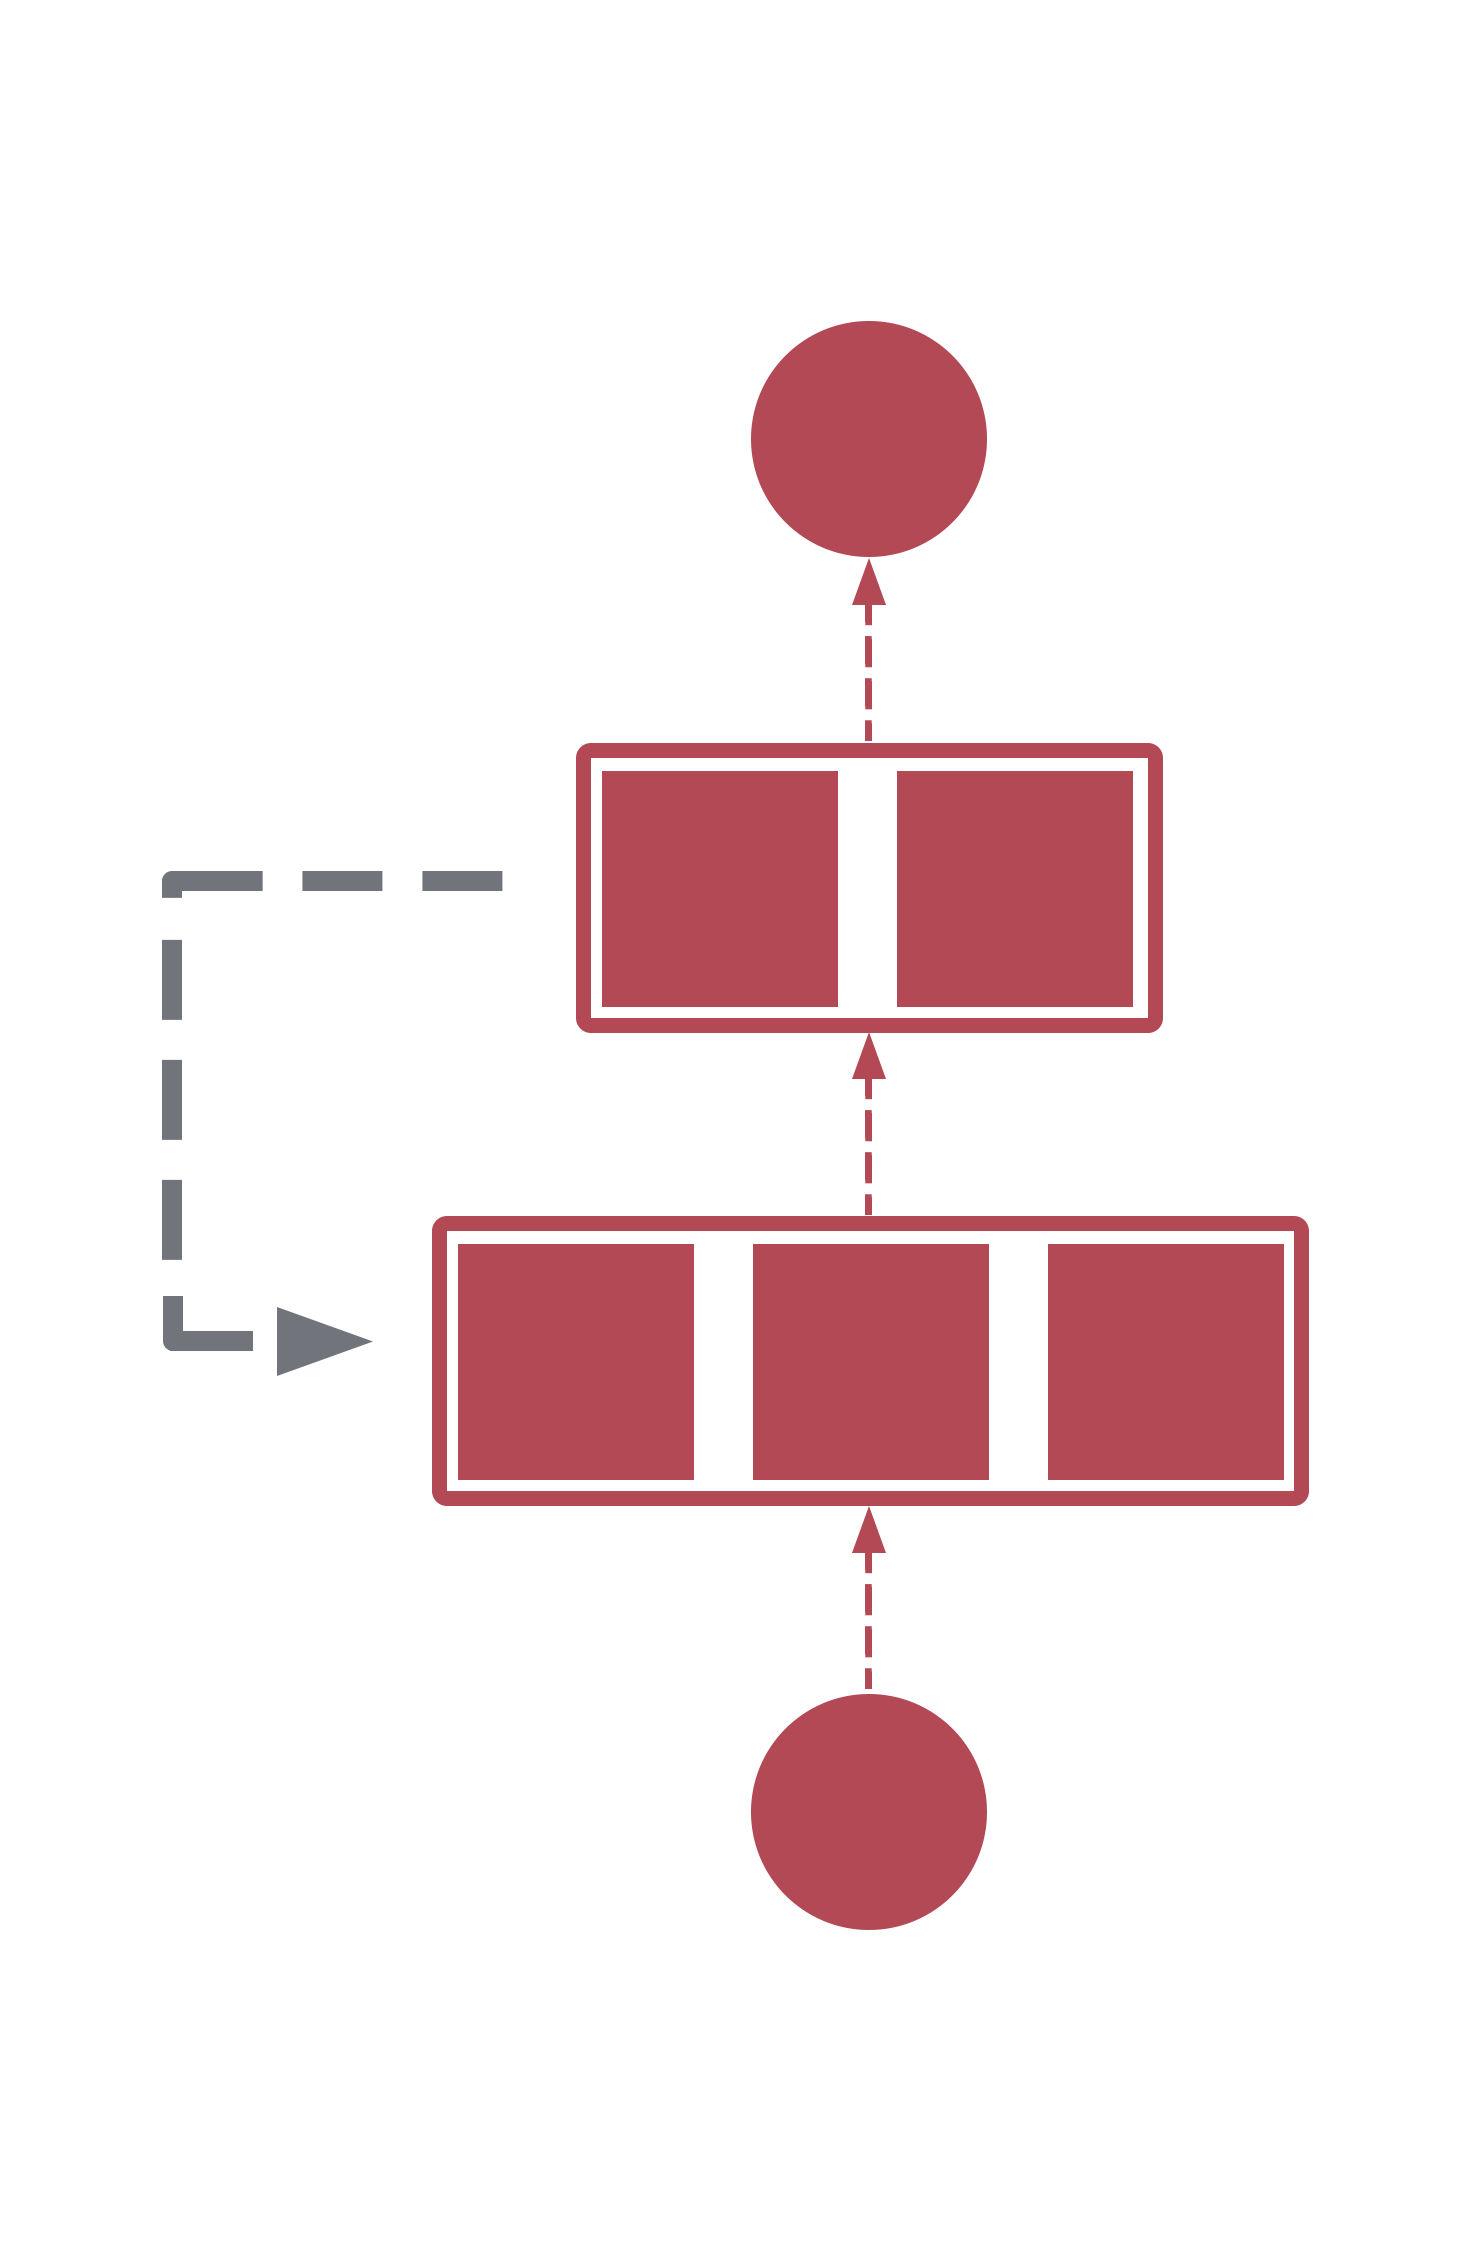
\includegraphics[width=0.6\textwidth]{rnn_schema}
        \caption{Schematic representation of a recurrent neural network.}
    \end{minipage}
\end{figure}

An example of FNN is the function obtained by chaining three components $f^{(1)}$, $f^{(2)}$ and $f^{(3)}$, yielding $f(\bm{x}) = f^{(3)}(f^{(2)}(f^{(1)}(\bm{x})))$. In this case, $f^{(1)}$ is called the \textit{first layer} of the network, $f^{(2)}$ is the \textit{second layer} and $f^{(3)}$, the final layer, is the \textit{output layer}. The overall length of the chain gives the \textit{depth} of the model. Training examples specify directly only what the output layer should return, with no clue on the behaviour of other layers. It is up to the ML algorithm to decide how to use those layers to produce the desired output that approximates $f^*$, the target function to learn, of interest for the given ML task. For this reason, they are called \textit{hidden layers}. 

Hidden layers are usually vector-valued and their dimensionality determines the \textit{width} of the model. Every element of the vector may be interpreted as a human neuron and the layer can be considered as consisting of many \textit{units} that act in parallel, each representing a vector-to-scalar function. Each unit resembles a neuron since it receives inputs from many other connected units (or from the external environment, in case of the first layer) and then computes its own activation value. However, the goal of ANNs is not to perfectly model the brain, even though the choice of the some layer functions $f^{(i)}$ is sometimes guided by neuroscientific observations on biological neurons.

ML tasks often require to learn a nonlinear function $f^*$. In order to compute a nonlinear function of $\bm{x}$ at least one layer $f^{(i)}$ of the ANN must involve a nonlinear transformation, otherwise the final output of the network would remain a linear combination of its intermediate results. Most FNNs rely on an affine transformation on every hidden layer, followed by a fixed nonlinear function called \textit{activation function}. The output layer, on the contrary, does not usually apply any further nonlinear transformation. As a result, every hidden layer consists of a vector of hidden units $\bm{h}^{(i)}$ computed by the corresponding nonlinear function $f^{(i)}(\bm{x}; \bm{W}^{(i)}, \bm{c}^{(i)})$, where $\bm{W}^{(i)}$ provides the weights of the linear transformation and $\bm{c}^{(i)}$ the biases. The network thus computes the values of some hidden units and then uses them as input for the next layer. By doing so, information flows in a unidirectional way from one hidden layer to the next, up to the output layer. This is the reason why this kind of neural network is called feedforward.

The computational process of a FNN just described can be now formally defined. Given a FNN $f : \mathbb{X} \to \mathbb{Y}$ composed by $n$ functions (layers) $f^{(1)}$, $f^{(2)}$, ..., $f^{(n-1)}$, $f^{(n)}$, we have

\begin{equation}
\label{eq:ANN_compact}
f(\bm{x}) = f^{(n)}(f^{(n-1)}(...(f^{(2)}(f^{(1)}(\bm{x}))))),
\end{equation}

where
\begin{equation}
\label{eq:ANN_layers}
f^{(i)}(\bm{x}) =
\begin{cases}
    g^{(i)}(\bm{W}^{(i)\top} \bm{x} + \bm{c}^{(i)}) & \text{if i} = 1\\
    g^{(i)}(\bm{W}^{(i)\top} f^{(i-1)}(\bm{x}) + \bm{c}^{(i)}) & \text{otherwise}
\end{cases},
\end{equation}

with $g^{(i)}$ arbitrary activation functions, $\bm{W}^{(i)}$ layers weights and $\bm{c}^{(i)}$ layers biases.

For convenience, all these parameters are usually grouped in a vector $\bm{\theta}$. Training an ANN amounts to finding a $\bm{\theta}$ such that   $f(\bm{x}; \bm{\theta})$ well approximate $f^*(\bm{x})$. This is usually done with information provided by a \textit{loss function}.



\subsection{Loss functions}

In mathematical optimization, a loss function $l : \mathbb{A} \to \mathbb{R}$ assigns a cost to an event or value. This number intuitively measures how bad the effects of an event are or how distant is the input value from the target one. An optimization problem obviously seeks to minimize the loss function. In some cases, the objective function is the opposite of $l$, it is called \textit{reward function}, and the equivalent goal is to maximize it.

The loss functions of ANNs are similar to those of other parametric models. In most cases, a network defines a distribution $p(\bm{y} | \bm{x}; \bm{\theta})$, so it is possible to estimate $\bm{\theta}$ via \textit{maximum likelihood estimation}, a popular method of estimating statistical model parameters given observations. 

ANNs are thus often trained using the cross entropy between the empirical distribution defined by the training set $\hat{p}_{data}$ and the model distribution $p_{model}$:

\begin{equation}
l(\bm{\theta}) = - \mathbb{E}_{\bm{x}, \bm{y} \sim \hat{p}_{data}} \log p_{model}(\bm{y}|\bm{x}),
\end{equation}

where $l$ is the loss function associated to the entire network.

An advantage of deriving the loss function from maximum likelihood is that it removes the burden of designing a new loss function for each model: specifying a model $p_{model}(\bm{y} | \bm{x})$ automatically determines a cost function $\log p_{model}(\bm{y} | \bm{x})$.

Regardless of which loss function is chosen to train the model, the minimization of the error is achieved through an optimization method, such as \textit{gradient descent}. For such reason, the loss function must be differentiable. In addition, in order to serve as a good guide throughout all the training algorithm, its gradient should always be large and predictable. Functions that saturate undermine this objective because they produce very small gradients. In many cases
this happens because the activation functions used to compute the output of the hidden units or the output units saturate. The logarithm in the negative log-likelihood loss function succeeds in undoing the problematic effect caused by output units involving exponential functions that saturate when their argument is very small.

Error minimization through gradient descent \cite{hadamard1908memoire} in the parameters space of
complex, nonlinear, differentiable systems has been discussed at least since the early 1960s, initially within the framework of Euler-Lagrange equations in the calculus of variations \cite{Euler:1744}. However, an efficient procedure to minimize loss functions was first described only a decade later \cite{Linnainmaa:1970}\cite{Linnainmaa:1976}, with the design of the algorithm of \textit{backpropagation}.



\subsection{Backpropagation}

Backpropagation is an efficient method used during ANNs training to compute how weights connecting units should be updated with respect to the value of the loss function.
The systems of the 1960s transmitted derivative information through standard Jacobian matrix calculations from one ``layer'' to the previous one, without explicitly addressing either direct links across several layers or potential additional efficiency gains due to network sparsity, typical of ANNs.
Modern backpropagation overcomes these limitations with a computational cost essentially equivalent of the forward pass.

Equations \eqref{eq:ANN_compact} and \eqref{eq:ANN_layers} concisely describe how ANNs layers as a whole interact with each other. However, to easily describe the backpropagation algorithm, it is handy to define some additional ones that involve single units.

We define $w_{i,j}$ as the weight connecting two units $h_i$ and $h_j$ belonging to different layers. $\mathbb{W}$ is the set of such weights. An iterative optimization algorithm should try to optimize each $w_{i,j}$, step by step, according to the error measured by $l$. This is done with gradient descent in the following way:

\begin{equation}
w_{i,j} \gets w_{i,j} - \eta \frac{\partial l}{\partial w_{i,j}},
\end{equation}

where $\eta \in \mathbb{R}$ is the \textit{learning rate}.

We define $pred_j$ as the set of input units connected to $h_j$:

\[
pred_j = \{h_i | w_{i,j} \in \mathbb{W} \}
\]

and, similarly, $succ_j$ as the set of output units connected to $h_j$:

\[
succ_j = \{h_i | w_{j,i} \in \mathbb{W} \}
\]

Supposing a fixed differentiable activation function $\varphi$ for every unit, we define $net_j$ as the input $h_j$ receives from the units it is connected to:

\[
net_j = \sum\limits_{k}^{pred_j} w_{k,j} \cdot o_k,
\]

where $o_k = \varphi(net_k)$ is the output of $h_k$. If the unit $h_k$ is in the first layer after the input layer, than $o_k$ is just $\bm{x}_k$, with $\bm{x}$ being a training example.

Each weight $w_{i,j}$ should be updated according to:

\begin{equation}
\label{eq:bp_final}
\frac{\partial l}{\partial w_{i,j}} = \delta_j \cdot o_i,
\end{equation}

where
\[
\delta_j =
\begin{cases}
     \frac{\partial l}{\partial f(\bm{x}_j)} \cdot \varphi\prime(net_j) & \text{if unit $h_j$ in output layer} \\ \\
     \sum\limits_{k}^{succ_j} \delta_k \cdot w_{j,k} \cdot \varphi\prime(net_j) & \text{otherwise}
\end{cases}.
\]

The full derivation of \eqref{eq:bp_final} can be found in appendix \ref{sec:appendix_backprop}.

The resulting iterative procedure to train an ANN via gradient descent is described by algorithm \ref{alg:gradient_descent}.

\begin{algorithm}
\caption{Gradient descent algorithm to train an ANN}
\label{alg:gradient_descent}
\begin{algorithmic}[1]
\Require ANN $f$
\Require initialized set of weights $\mathbb{W}$
\Require loss function $l$
\Require learning rate $\eta$
\While {the stopping criterion is not satisfied} \label{line:criterion}
    \ForAll {training examples $(\bm{x}, \hat{\bm{y}})$} \label{line:x_loop}
        \State $\bm{y} \gets f(\bm{x})$
        \Comment compute ANN output
        \ForAll {weight $w_{i,j} \in \mathbb{W}$}
            \State $\Delta w_{i,j} \gets \delta_j \cdot \bm{y}_i$ 
            \Comment see equation \eqref{eq:bp_final} 
            \State $w_{i,j} \gets w_{i,j} - \eta \Delta w_{i,j}$
            \Comment update weight according to loss
        \EndFor
    \EndFor
\EndWhile
\end{algorithmic}
\end{algorithm}

During the initialization phase, weights are usually given small random values. The stopping criterion (line \ref{line:criterion}) can be any predicate reasonable for the learning task, such as \textit{all training examples are classified correctly} or \textit{the error computed by the loss function $l$ is below a given threshold}. This procedure is usually repeated several times; the number of times training examples are used once to update the weights is an \textit{epoch}.

Many widely adopted techniques in DL are discovered empirically and systematically applied because they work well in practice, even if their theoretical background is still uncertain and sometimes it happens to see little algorithmic tricks that effectively improve the overall performances of the ANNs. In the same way, it is also common to see approximations that make computation faster or even feasible, without a significant loss in performance. For instance, the gradient descent algorithm is usually modified to process little groups of training examples, called \textit{mini-batches}, instead of one example at a time (line \ref{line:x_loop}) or by randomly shuffling the training set at each new iteration (line \ref{line:criterion}), giving rise to the \textit{stochastic gradient descent algorithm} (algorithm \ref{alg:stochastic_gradient_descent}). It is now worth pointing out some other theoretical considerations.

\begin{algorithm}
\caption{Stochastic gradient descent algorithm to train an ANN}
\label{alg:stochastic_gradient_descent}
\begin{algorithmic}[1]
\Require ANN $f$
\Require initialized set of weights $\mathbb{W}$
\Require loss function $l$
\Require learning rate $\eta$
\Require mini-batch size $m$
\While {the stopping criterion is not satisfied}
    \State $mb \gets$ data mini-batch \{$(\bm{x}^{(1)}, \hat{\bm{y}}^{(1)})$, $(\bm{x}^{(2)}, \hat{\bm{y}}^{(2)})$, ..., $(\bm{x}^{(m)}, \hat{\bm{y}}^{(m)})$\} randomly sampled from training set 
    \For{$k \gets 1, m$}
        \State $\bm{y}^{(k)} \gets f(mb_k[\bm{x}])$
        \Comment compute ANN outputs
    \EndFor
    \ForAll {weight $w_{i,j} \in \mathbb{W}$}
        \State $\Delta w_{i,j} \gets 0$
        \For{$k \gets 1, m$}
        \State $\bm{x} \gets mb_k[\bm{x}]$
        \State $\bm{y} \gets \bm{y}^{(k)}$
            \State $\Delta w_{i,j} \gets \Delta w_{i,j} + \delta_j \cdot \bm{y}_i$ 
            \Comment see equation \eqref{eq:bp_final}
        \EndFor
        \State $w_{i,j} \gets w_{i,j} - \eta \cdot \frac{1}{m} \cdot \Delta w_{i,j}$
        \Comment update weight according to average loss
    \EndFor
\EndWhile
\end{algorithmic}
\end{algorithm}


\subsection{Theoretical considerations}

A number of considerations about DL should be kept in mind when designing ANNs.

First of all, the \textit{``no free lunch'' theorem} for ML \cite{nfl} states that, averaged over all possible data generating distributions, every classification algorithm has the same error rate when classifying previously unobserved examples. In other words, no ML algorithm is universally any better than any other. However, the goal of ML research is not to seek a universal learning algorithm, but to design systems that perform well on specific tasks. For such reason, there is no need to average over all possible data distributions, since only a tiny subset of them are relevant for the real world we experience. The theorem suggests that ML algorithms should be developed by encoding a set of preferences into the learning algorithm itself. If this is done appropriately, than the algorithm will solve the task it is designed for.

Secondly, the central challenge in ML is generalization. The generalization error of a ML model is typically estimated by measuring its performance on a test set of examples unavailable during training. The factors determining how well a ML algorithm will perform are its abilities to make both the training error and its gap with the test error small. These two factors correspond to two known problems in ML: \textit{underfitting} and \textit{overfitting}. The former occurs when the model is not able to obtain a sufficiently low error value on the training set, the latter when the gap between the training error and the test error is too large. One can control whether a model is more likely to overfit or underfit by altering its \textit{capacity}, the ability to fit a wide variety of functions. What should be kept in mind is that, typically, as model capacity increases, training error decreases until it asymptotes to the minimum possible value, while generalization error has a U-shaped curve and, after a certain point, it will start increasing. With \textit{regularization} it is possible to reduce the generalization error without any impact on the training error.


\begin{figure}[ht]
\centering
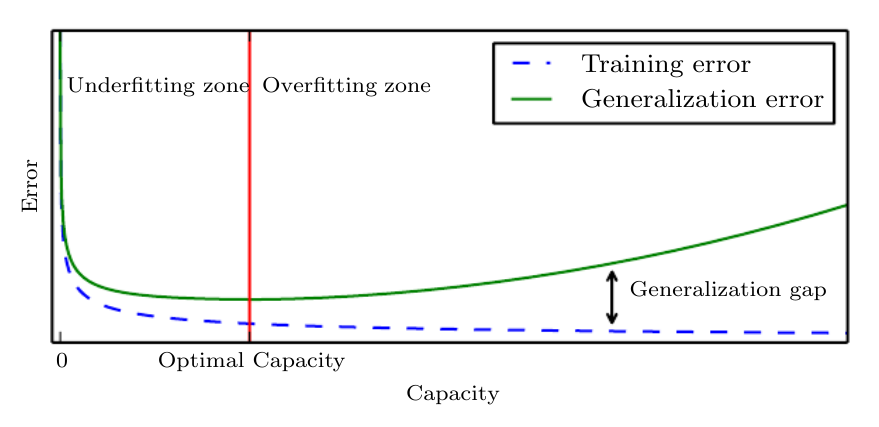
\includegraphics[width=0.8\textwidth,keepaspectratio]{errors}
\caption{Typical relationship between capacity and error as illustrated in \cite{The_DL_book}. At the left end of the graph, training error and generalization error are both high, in the underfitting regime. As capacity increases, training error decreases, but the gap between training and generalization error increases. Eventually, the size of this gap outweighs the decrease in training error and overfitting regime is reached.}
\end{figure}


A final considerations regards \textit{hyperparameters}, a set of values defining higher level concepts about the model, such as the network learning rate. Since they cannot be learnt directly from the training data, they are usually empirically found by testing different models on a validation set, another set of data unavailable during training, and then selecting the best ones. Hyperparameters tuning can be expensive and is an active research field since these values can largely impact on the final performance of the network.
% TODO ref




\section{Deep generative models}


ML models are typically divided into two complementary classes: \textit{discriminative models} and \textit{generative models}. From a probabilistic point of view, discriminative methods try to learn a mapping from input variables $x$ to output variables $y$ directly modelling the conditional probability distribution $p(y|x)$. On the contrary, generative methods try to learn the joint probability distribution $p(x, y)$ underlying the data. Since $p(x, y)$ can be used to compute $p(y|x)$, generative models can also be used to make predictions. However, probably due to the easier nature of their goal, discriminative algorithms often achieve better results in classification tasks and are generally preferred \cite{disc_vs_gen}. Nevertheless, generative models are actively studied because of their peculiar capability of generating new data resembling those in input once $p(x, y)$ is learnt.

Some generative models allow the probability distribution function to be evaluated explicitly, while others only support operations that implicitly require knowledge of it, such as sampling. Techniques to automatically learn an approximation of the real data distribution are particularly useful when learning the exact one is hard or even impossible. Indeed, modern generative networks, when given enough training examples and capacity, often succeed in learning a distribution very similar to the true one. The key insight is that ANNs used for generative models are forced to learn representations in a space significantly smaller than the one of training data and so they are forced to learn meaningful features in order to later generate new data.

\begin{figure}[ht]
\centering

\includegraphics[width=0.8\textwidth,keepaspectratio]{handwritten}
\caption{Different examples of the words sequence ``that a doctor should be'' drawn from a RNN generator \cite{handwritten_rnn}.}
\end{figure}

It is likely that in the near future ANNs will be able to generate samples depicting entirely plausible images or videos. This may by itself find use in multiple applications, such as on-demand generated art \cite{igan} \cite{furniture} (see figure \ref{fig:art_on_demand}). However, one important application of these networks is the generation of synthetic data to augment real data sets, especially for pre-training, a procedure during which the model is trained in advance on data similar to those of the task to avoid random network parameters initialization.
% Nevertheless, it is worth pointing out that no model will ever be able \todor{to generate examples of things it has never seen real examples of before}{troppo generico, non accurato}.
Besides these speculations, present known applications include image denoising, inpainting \cite{inpainting}, super-resolution \cite{growing_gans} \cite{super_gans}, exploration in reinforcement learning and neural network pre-training in cases where labelled data are expensive.

\begin{figure}[ht]
    \centering
    \begin{minipage}{0.32\textwidth}
        \centering
        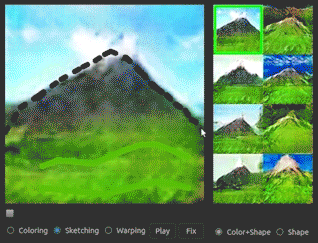
\includegraphics[width=\textwidth]{igan1}
    \end{minipage}
    \begin{minipage}{0.32\textwidth}
        \centering
        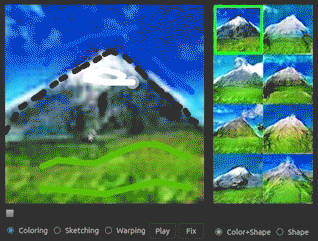
\includegraphics[width=\textwidth]{igan2}
    \end{minipage}
    \begin{minipage}{0.32\textwidth}
        \centering
        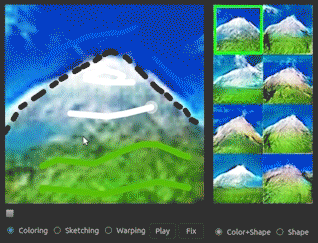
\includegraphics[width=\textwidth]{igan3}
    \end{minipage}
    \caption{Example of interactive image generation from \cite{igan}. A system can produce photo-realistic samples that best satisfy the user edits in real-time.}
    \label{fig:art_on_demand}
\end{figure}


This work focuses on a family of generative models called \textit{generative adversarial networks}.


\subsection{Generative adversarial networks}


% "Adversarial training is the coolest thing since sliced bread." - Yann LeCun, Director of AI Research at Facebook and Professor at NYU

Generative adversarial networks (GANs) are based on a game theoretic scenario in which two networks, a \textit{discriminator} and a \textit{generator}, compete against each other. The goal of the generator is to produce objects similar to the training examples and trick the discriminator into believing they are real. This model can be thus thought as a game between a counterfeiter, trying to produce fake currency, and a policeman, trying to detect it. The idea to infer models in a competitive setting was first used for behavioural inference in the field of ethology \cite{controlled_interaction} and to find binary factorial codes \cite{factorial_codes}.

Formally, we define the discriminator as a network $D(\bm{x}; \bm{\theta}^{(d)})$ and the generator as a network $G(\bm{z}; \bm{\theta}^{(g)})$, where $\bm{z}$ is a random input noise drawn from a distribution $p_z$. We define the generator's probability distributions over data $\bm{x}$ as as $p_g$.

The output of the generator $\bm{x}=G(\bm{z})$ represents a generated object that should resemble those of the training set, while the output of the discriminator $y=D(\bm{x})$ represents the probability that $\bm{x}$ was sampled from $p_{data}$ rather than $p_g$.

The goal of the model is to train simultaneously $D$ and $G$: the discriminator should try to maximize its output probabilities for training examples; the generator should try minimize the probability of generating objects that will be rejected by $D$ (i.e. those receiving a low score). So, $D$ and $G$ play the following minimax game with \textit{value function} $V(D, G)$:

\begin{equation}
\min_G \max_D V(D, G).
\end{equation} 

A typical choice for $V(D, G)$ is

\begin{equation}
V(D, G) = \underbrace{\mathbb{E}_{\bm{x} \sim p_{data}} [\log D(\bm{x})]}_\textrm{\textit{D} goal} + \underbrace{\mathbb{E}_{\bm{z} \sim p_z} [\log (1 - D(G(\bm{z})))]}_\textrm{\textit{G} goal}.
\end{equation}

However, when $G$ has not learnt yet how to produce good objects, $D$ can reject samples from $p_g$ with high confidence. In this case $\log (1 - D(G(\bm{z})))$ saturates, preventing learning. To avoid this issue, $G$ can be instead trained to maximize the opposite function, $\log D(G(\bm{z}))$. Although mathematically equivalent, the second formulation provides better gradients in early training.

\begin{figure}[ht]
    \centering
    
\includegraphics[width=0.7\textwidth]{gan_schema}
    \caption{Schematic representation of GANs with a generator (blue) producing objects for the discriminator (red).}
\end{figure}

In practice, $D$ and $G$ are trained via traditional backpropagation using an iterative approach consisting of two alternating loops of $k$ steps of $D$ optimization and one step of $G$ optimization. This results in $D$ being maintained near its optimal solution as long as $G$ changes slowly enough. Algorithm \ref{alg:sgd_gans} shows the mini-batch stochastic gradient descent training procedure for GANs.

\begin{algorithm}
\caption{Stochastic gradient descent algorithm to train GANs}
\label{alg:sgd_gans}
\begin{algorithmic}[1]
\Require ANN discriminator $D$
\Require ANN generator $G$
\Require discriminator parameters $\bm{\theta}^{(d)}$
\Require generator parameters $\bm{\theta}^{(g)}$
\Require learning rate $\eta$
\Require mini-batch size $m$
\Require discriminator training steps number $k$
\While {the stopping criterion is not satisfied}
    \For {$k$ steps}
        \State $z\_mb \gets$ noise mini-batch \{$\bm{z}^{(1)}$, $\bm{z}^{(2)}$, ..., $\bm{z}^{(m)}$\} randomly sampled from $p_z$
        \State $mb \gets$ data mini-batch \{$\bm{x}^{(1)}$, $\bm{x}^{(2)}$, ..., $\bm{x}^{(m)}$\} randomly sampled from $p_{data}$
        \State $\Delta \bm{\theta}^{(d)} \gets \nabla_{\bm{\theta}^{(d)}} \frac{1}{m} \sum\limits_{i=1}^m [\log D(mb_i) + \log (1 - D(G(z\_mb_i)))]$
        \Comment compute gradient
        \State $\bm{\theta}^{(d)} \gets \bm{\theta}^{(d)} + \eta \Delta \bm{\theta}^{(d)}$ 
        \Comment update D by ascending gradient
    \EndFor
    \State $z\_mb \gets$ noise mini-batch \{$\bm{z}^{(1)}$, $\bm{z}^{(2)}$, ..., $\bm{z}^{(m)}$\} randomly sampled from $p_z$
    \State $\Delta \bm{\theta}^{(g)} \gets \nabla_{\bm{\theta}^{(g)}} \frac{1}{m} \sum\limits_{i=1}^m [\log (1 - D(G(z\_mb_i)))]$
    \Comment compute gradient
    \State $\bm{\theta}^{(g)} \gets \bm{\theta}^{(g)} - \eta \Delta \bm{\theta}^{(g)}$ 
    \Comment update G by descending gradient
\EndWhile
\end{algorithmic}
\end{algorithm}


In a scenario in which the two networks have access to infinite examples, after several training steps, if $G$ and $D$ have enough capacity, they will reach a point at which both cannot improve because $p_g = p_{data}$. In this situation the discriminator will be unable to differentiate between the two distributions and every example will have the same probability of being real or generated, i.e. $D(\bm{x}) = \frac{1}{2}$. In general, given a fixed generator $G$, the optimal discriminator is

\begin{equation}
\label{perfect_gans_D}
D^*_G(\bm{x}) = \frac{p_{data}(\bm{x})}{p_{data}(\bm{x}) + p_g(\bm{x})}
\end{equation}

The main motivation for the design of GANs is that the learning process
requires neither approximate inference nor approximation of a partition function gradient, but only traditional backpropagation. Furthermore, the model is very flexible since $D$ and $G$ can be any ANN and eliminates the need of Markov chains.

On the other side, GANs do not offer an explicit representation of $p_g$. Furthermore, some critical issues may be hidden in the training procedure. First, $D$ and $G$ must be synchronized well in order to avoid the scenario in which the generator collapses too many values of $\bm{z}$ to the same value of $\bm{x}$. This usually happens when $G$ is trained too much, without updating $D$. Second, simultaneous gradient descent in the adversarial game setting is not guaranteed to reach an equilibrium. In fact, it is possible for the two players to take infinite turns increasing and then decreasing the value function forever, rather than landing exactly on the saddle point of $V$ where they cannot further reduce their costs. Note that the equilibria for a minimax game are not local minima of $V$, but saddle points which are local minima with respect to the first player’s parameters and local maxima with respect to the second player’s parameters. Finally, GANs framework is designed for fully differentiable networks $D$ and $G$. This is problematic since many important real-world data sets, such as word-base representations of language, are discrete. However, there exist variants that can deal with discrete variables, such as \textit{boundary-seeking generative adversarial networks}.



\subsection{Boundary-seeking generative adversarial networks}

Boundary-seeking generative adversarial networks (BGANs) provide a unified framework to deal with discrete and continuous variables. For the present work, only the former are of interest and will be further analysed.

Given a fixed generator $G$, from equation \eqref{perfect_gans_D} it is possible to derive the density of data:

\begin{equation}
p_{data}(\bm{x}) = p_g(\bm{x}) \frac{D^*_G(\bm{x})}{1 - D^*_G(\bm{x})}.
\end{equation}

This indicates that, in the limit of a perfect discriminator $D^*$, the true data distribution can be perfectly estimated from such discriminator and any fixed generator $G$, even if that generator is not perfectly trained. A sample from the correct data distribution can thus be obtained by simply reweighing samples drawn from the imperfect distribution $p_g$ according the ratio $\frac{D^*_G(\bm{x})}{1 - D^*_G(\bm{x})}$.

Unfortunately, it is unlikely that the perfect discriminator $D^*$ can be learnt or even exists. However, given an imperfect discriminator $D$, the true data distribution $p_{data}$ can be approximated in the following way:

\begin{equation}
\label{eq:p_data_estimator}
\widetilde{p}_{data}(\bm{x}) = \frac{1}{Z} p_g(\bm{x}) \frac{D(\bm{x})}{1 - D(\bm{x})},
\end{equation}

where

\[
Z = \sum\limits_{\bm{x}} p_g(\bm{x}) \frac{D(\bm{x})}{1 - D(\bm{x})}
\]

is the normalization constant that guarantees $\widetilde{p}_{data}$ to be a proper probability distribution. The bias $\widetilde{p}_{data}$ is affected to only depends on the quality of $D$: the closer $D$ is to $D^*$, the lower the bias. This is a nice property, since training the discriminator (a standard probabilistic binary classifier) is generally easier than training the generator (whose objective function is a moving target as the discriminator adapts to the generator and vice versa). Note that the optimum for the generator occurs at $D(\bm{x}) = D^*(\bm{x}) = \frac{1}{2}$, so that $Z = 1$ and $p_{data} = \widetilde{p}_{data} = p_g$. This occurs at the decision boundary of the discriminator, when generated samples have the same probability of being classified as real data or samples. This is the reason for the name BGANs.

GANs have serious limitations on the type of variables they can model, because they require the composition of the generator and discriminator to be fully differentiable. With discrete variables this is not true. For instance, consider using a step function at the end of a generator in order to generate a discrete value. In this case, backpropagation alone cannot provide the training signal for the generator, since the derivative of a step function is $0$ almost everywhere and so would be the backpropagated signal. The goal of BGANs is to train a generator outputting discrete values by estimating gradients for $\bm{\theta}^{(g)}$ via the exclusive Kullback-Leibler divergence between the two joint distributions $p_{data}(\bm{x}, \bm{z})$ and $p_g(\bm{x}, \bm{z})$:

\begin{equation}
\nabla_{\bm{\theta}^{(g)}} D_{KL}(p_{data}(\bm{x}, \bm{z}) || p_g(\bm{x}, \bm{z})),
\end{equation}

or by using the biased estimator:

\begin{equation}
\label{eq:dkl_bgans}
\nabla_{\bm{\theta}^{(g)}} D_{KL}(\widetilde{p}_{data}(\bm{x}, \bm{z}) || p_g(\bm{x}, \bm{z})).
\end{equation}

The generator distribution $p_g(\bm{x})$ can be parametrized as the marginalization of a joint density
\begin{equation}
\label{eq:cond_prob_g}
p_g(\bm{x}) = \sum\limits_{\bm{z}} g(\bm{x}|\bm{z})p_z(\bm{z}), 
\end{equation}

where $g(\bm{x}|\bm{z})$ is the conditional distribution of the generator function.

The result of the computation of the gradient in equation \eqref{eq:dkl_bgans} is:

\begin{equation}
\label{eq:gradient_bgans}
\nabla_{\bm{\theta}^{(g)}} D_{KL}(\widetilde{p}_{data}(\bm{x}, \bm{z}) || p_g(\bm{x}, \bm{z})) \approx - \mathbb{E}_{\bm{z} \sim p_z(\bm{z})} [\sum\limits_{m = 1}^{M} \widetilde{w}^{(m)} \nabla_{\bm{\theta}^{(g)}} \log g(\bm{x}^{(m)} | \bm{z})],
\end{equation}

where
\[
\widetilde{w}^{(m)} = \frac{w^{(m)}}{\sum\limits_{m'} w^{(m')}} 
\]

and

\[
w^{(m)} = \frac{D(\bm{x}^{(m)})}{1 - D(\bm{x}^{(m)})} 
\]

are the normalized and unnormalized importance weights and $\bm{x}^{(m)}$ are samples from the generator for the given $\bm{z}$. The normalization can help to generate a relative learning signal that is particularly useful when samples are all fairly bad from the point of view of $D(\bm{x})$.

% TODO spiegare meglio la questione dei valori discreti. Guarda intro BGAN

This allows to compute gradients from a mini-batch of samples from $p_z(\bm{z})$ and to train discrete GANs without relying on backpropagation. Compared to normal GANs, this method requires $M$ times more space, but computing the $M$ (instead of $1$) scalar values of $D(\bm{x}^{(m)})$ can be parallelized, as samples from $g(\bm{x} | \bm{z})$ can be drawn independently.

The full derivation of \eqref{eq:gradient_bgans} can be found in appendix \ref{sec:appendix_bgans}.


\section{Constrained problems}

Many real-world applications involve domains subject to a set of constraints, such as grammar rules for sentences, design constraints for modelling, safety rules for airline protocols or game rules. These applications typically solve one of the two following kinds of problem: \textit{constraint satisfaction} or \textit{constrained optimization}.

A constraint satisfaction problems (CSP) is defined as a set of objects whose state must satisfy a number of constraints or limitations.
Formally, a CSP is defined as a triple $\langle \mathbb{X}, \mathbb{D}, \mathbb{C} \rangle$, where $\mathbb{X} = \{x^{(1)}, x^{(2)}, ..., x^{(n)}\}$ is a set of variables, $\mathbb{D} = \{D^{(1)}, D^{(2)}, ..., D^{(n)}\}$ is the set of the respective domains and $\mathbb{C} = \{c^{(1)}, c^{(2)}, ..., c^{(m)}\}$ is a set of constraints. Every constraint $c^{(i)} \in \mathbb{C}$ is a pair $\langle t^{(i)}, R^{(i)} \rangle$, where $t^{(i)} \subseteq \mathbb{X}$ is a subset of $k$ variables and $R^{(i)}$ is a $k$-ary relation on the corresponding subset of domains. A solution to the CSP is an assignment of values from $\mathbb{D}$ to all the variables in $\mathbb{X}$ that satisfies all the constraints in $\mathbb{C}$.

CSPs are the subject of intense research in both AI and operations research since the regularity in their formulation often provides a common basis to solve seemingly unrelated problems. Propositional satisfiability problem (SAT), satisfiability modulo theories and answer set programming can be thought as instances of CSPs. Classic examples of CSPs are the eight queens puzzle, the map colouring problem and Sudoku.

Constrained optimization problems (COPs) involve the process of finding the best values for an objective function with respect to some variables in the presence of constraints on those variables. The objective function is either a cost function to be minimized or a reward function to be maximized. Constraints can be either hard (variables must satisfy them) or soft (variables may not satisfy them with a penalization in the objective function). More formally, a general constrained minimization problem is expressed as

\begin{equation*}
\begin{aligned}
& \text{min} & & f(\bm{x}) & & & \\
& \text{subject to} & & g_i(\bm{x}) = c_i & \text{for $i = 1, ..., n$} & & \text{equality constraints} \\
&&& h_j(\bm{x}) > d_j & \text{for $j = 1, ..., m$} & & \text{inequality constraints}
\end{aligned}
\end{equation*}

Optimization can be an extremely difficult task. ML algorithms try to avoid these difficulties by adopting particular objective functions and constraints to ensure that the optimization problem is convex. When training ANNs, optimization is generally performed in the non-convex case and this can cause many issues, such as finding only local minima.

Many techniques and software exist to solve CSPs and COPs, but their analysis is out of the scope of this work.

    \chapter{Constrained adversarial networks}
\label{ch:can}

\begin{flushright}
\rightskip=.8cm\textit{``What I cannot create, I do not understand.''} \\
\vspace{.2em}
\rightskip=.8cm Richard Feynman
\end{flushright}
\vspace{1em}


Though there exist general frameworks that allow the encoding of various structured constraints on latent variable models \cite{slvm_pr} \cite{bayesian_pr} \cite{exp_learn}, they either are not directly applicable to ANNs or yield inferior performance \cite{harnessing}.
Constrained adversarial networks (CANs) are a generalization of the deep generative model of BGANs, designed to introduce constraints during the adversarial training. The goal of the model is to train a generator that will be able to produce samples that simultaneously resemble those in the training set and satisfy a set of input constraints in expectation.

More formally, CANs consist of a discriminator network $D(\bm{x}; \bm{\theta}^{(d)})$, a generator network $G(\bm{z}; \bm{\theta}^{(g)})$ and a set of constraints $\mathbb{C} = \{c^{(1)}, c^{(2)}, ..., c^{(m)}\}$, where each constraint $c^{(i)}: \mathbb{X} \to [0, 1]$ is a penalty function. Consistently with GANs, we define $\bm{z}$ as a random input noise drawn from a distribution $p_z$, and $p_g$ as the generator's probability distributions over data $\bm{x}$. The output of the generator $\bm{x}=G(\bm{z})$ represents a generated object resembling those of the training set and, possibly, satisfying the constraints, while the output of the discriminator $y=D(\bm{x})$ represents the probability that $\bm{x}$ was sampled from $p_{data}$ rather than $p_g$. In addition, we define a \textit{perfect} object as follows:

\begin{Definition}
    Given a set of constraints $\mathbb{C}$, an object x is perfect if $c(x) = 0$ $\forall c \in \mathbb{C}$.
\end{Definition}


\section{Theoretical motivations}

The design of CANs is guided by some theoretical motivations regarding common issues arising when dealing with domains subject to constraints. One of them is that formally encoding constraints may sometimes be hard. This problem is especially true when constraints involve global properties of objects that we, as human, recognize intuitively or can not formally describe. In particular, a constraint can be hard to encode either from a \textit{practical} point of view or from a \textit{conceptual} one. For instance, suppose our data set is made up of images of human faces. A constraint that is practically hard to encode may involve the expected number of eyes on each image. Expressing such property in term of image pixels is clearly unfeasible. However, it is very simple for us to describe what high-level image characteristics we expect to consider the constraint satisfied and, even simpler, to determine if the constraint is not satisfied from a quick glance. On the contrary, it is conceptually harder for us to express the property of beauty. This is not something related to personal taste, rather to the global and somehow implicit nature of some image properties. Nevertheless, we expect a generative model to produce beautiful faces if its training set only consist of pictures of beautiful faces.

GANs are not affected by this problem because, when provided with enough capacity, they can automatically learn how to generate images resembling input data. So, if training set objects satisfy these high-level constraints, the generator will be forced to learn them in order to deceive the discriminator. As a final result, images sampled from $p_g$ will tend to have these desired properties even if they were not explicitly encoded anywhere. CANs inherit this capability from GANs. In addition, they provide the possibility to directly encode all the other constraints that can be easily expressed to instil external knowledge in the network and to guide the generator training process via penalty functions.

Finding solutions to constrained problem such as CSPs and COPs can be computationally hard. For instance, it is known that SAT is a decision problem NP-complete. The novel approach of CANs consists in replacing the explicit constraints optimization with an implicit polynomial-time learning procedure. During training, in particular, penalty function are evaluated by one of the two networks and their output values are used to guide the generator in better approximating with its probability distribution $p_g$ the goal distribution $p_{data}$. Exploring different solutions to make this idea effective and efficient has been the research goal.  Furthermore, once the networks are trained, generating a possibly perfect object only requires one forward passing of noise through the generator, so it can be done in polynomial-time as well. Also this property of the model is inherited by GANs.

Finally, in some situations finding a single solution is not sufficient for the task being performed and one may be interested in different candidates among those available, perhaps with some kind of statistical guarantee. Many methods are not designed to satisfy this requirement and obtaining different solutions may be particularly inefficient or even impossible. A generative model parametric on some input noise overcomes this limitation by its very nature. In fact, once trained, CANs can be efficiently used for sampling many instances from $p_g$ by simply using different input noise vectors $\bm{z}$. The more effective the ANNs training procedure is, the higher will be the number of perfect examples produced by the generator. However, the most important consideration involves execution times, since generating a possibly perfect object always requires polynomial time. This allows, for instance, efficient \textit{rejection sampling}, since CANs can be used to produce in polynomial time examples that, in expectation, will not be rejected, making this model useful for many other applications, such as approximate inference or recommendation. 


\section{Design choices}

Introducing constraints in the game theoretic scenario of GANs can be done in many different ways. This section describes some of the approaches that have been explored, postponing the presentation of the results and their analysis to chapter \ref{ch:experiments_and_results}.

\subsection{Adversarial models}

Since the adversarial training procedure involves two different networks, the first necessary design choice behind CANs regards the \textit{location} in which information coming from penalty functions should be used.

It would seem obvious to add constraints directly in the generator, since they can provide useful clues on how new objects shall be. In this case the generator loss function will include a signal on constraints satisfaction. The loss function to minimize of this new constraint-regularized generator may thus be
\[
l_G = \mathbb{E}_{\bm{z} \sim p_z} [\log (1 - D(G(\bm{z})))] + \lambda \mathbb{E}_{\bm{z} \sim p_z} [\sum\limits_{i=1}^{|\mathbb{C}|}c^{(i)}(G(\bm{z}))],
\]

where $\lambda$ is a regularization term.

This approach can be effective, but requires each constraint in $\mathbb{C}$ to be differentiable in order to backpropagate the learning signal throughout all the generator. Exploring this direction is left for future works.
    
The opposite approach is to introduce constraints in the discriminator network. Providing $D$ with some oracle penalty functions should enhance its capability to distinguish between training and sampled data. This is especially true when the training set only contains perfect objects. As long as the adversarial training is well-balanced, the generator will be indirectly forced to produce objects satisfying the constraints, especially during the first epochs. From a high-level point of view, this corresponds to strengthen the predictive capability of the discriminator that will, in turn, push the generator to produce better objects in order to effectively compete in the game. The objective function to maximize of this new constraint-regularized discriminator may thus be
\[
l_D = \mathbb{E}_{\bm{x} \sim p_{data}} [\log D(\bm{x}, \bm{c}(\bm{x}))] + \mathbb{E}_{\bm{z} \sim p_z} [\log (1 - D(G(\bm{z}), \bm{c}(G(\bm{z}))))] 
\]

This solution is conceptually reasonable and practically flexible. Furthermore, it is constraint-agnostic and can be used even with constraints that are not differentiable. For these reasons, it has been extensively tested.

Another approach is to extend the GANs model to introduce a third network, a \textit{teacher}, forcing the generator to emulate its rule-regularized predictions \cite{harnessing}. This iterative rule distillation process can effectively transfer rich structured knowledge, expressed in the declarative first-order logic language, into parameters of general neural network. Furthermore, this process is agnostic about the ANNs architectures and is left for future works as well.


\subsection{Discriminator architectures}

The second main design choice behind CANs involves the \textit{positioning} of constraints-related hidden units.

Regardless of the internal details about the discriminator architecture, the output layer will necessarily contains one single unit determining the final prediction on the input example. This characteristic enables a straightforward extension that is agnostic about the inner layers and thus applicable to any discriminator network. In this first approach, the original prediction $y = D(\bm{x})$ is linearly combined with a \textit{penalty vector} $\bm{c} = [c^{(1)}(\bm{x}), c^{(2)}(\bm{x}), ..., c^{(m)}(\bm{x})]$ and the final result $y'$ is given by a new output layer with a single unit receiving in input
\[
\alpha_0y + \sum\limits_{i=1}^m \alpha_i\bm{c}_i,
\]
where $\alpha_i$ are trainable weights balancing the importance of resembling input data and satisfying constraints. Since the output of the discriminator $y'=D(\bm{x})$ represents the probability that $\bm{x}$ came from $p_{data}$  rather than $p_g$ and constraints are evaluated via penalty functions assigning greater values to imperfect object, such as those produced by $p_g$, CANs should automatically learn to assign negative values to all the weights $\alpha_i$. By doing so, the more an input object violates the constraints, the easier it will be predicted as sampled. Perfect objects from training set will incur in no penalization during all the training procedure, regardless of the current values of $\alpha_i$, since their penalty vectors will always contain only $0$ values. In addition, CANs are given the possibility to learn which constraints are more useful during training since they can assign different scores to the multipliers $\alpha_i$.

A similar approach consists in using the same penalty vector in an inner layer, before the final output of the discriminator is computed. Of course, such approach is no more agnostic about the inner architecture of the ANN, thus possibly making CANs no more generally applicable around any black-box network $D$. However, in practice, the requirements to apply this method are easily met since it is reasonable to believe that any network $D$ will have a final hidden layer with some dozens of hidden units. More formally, given a discriminator $D(\bm{x}) = f^{(n)}(f^{(n-1)}(...(f^{(2)}(f^{(1)}(\bm{x})))))$ composed of $n$ layers, the final result $y'$ is given by the same output layer $f^{(n)}$ receiving in input
\[
f^{(n-1)}(\sum\limits_{i=1}^u \beta_u \bm{h}_u + \sum\limits_{i=1}^m \alpha_i\bm{c}_i),
\]

where $u$ is the number of hidden units of the last inner layer and $\bm{h} = f^{(n-2)}(...(f^{(2)}(f^{(1)}(\bm{x}))))$ is the the output of the previous hidden layer. The rationale behind this design trick is to slightly increase the impact of penalty vectors, exploiting them before the final decision is computed by the discriminator. Overall, the new discriminator has higher capacity than the one of the first approach and it is the one tested.


\subsection{Constraints timing}
\label{subsec:constraints_timing}

The last important design choice for CANs regards \textit{time intervals} in which hints from penalty functions should be actively used to train the model. The following considerations hold regardless of other design choices, such as those involving alterations of the training procedure or the ANNs architectures. Furthermore, they can be crucial for the final performance and efficiency of the model. This is especially true when evaluating penalty functions has a remarkable impact on execution times.

Many modern deep learning models are parametric on some conditions in order to dynamically change the function computed by the ANN in response to some events. For instance, some layers could be added, others could be dropped or some weights could be frozen for a certain period of time. This flexibility opens up a wide spectrum of possibilities.

The two time-related critical issues for CANs lie in the moment in which constraints should be introduced and in the duration for which they should be used. The number of combinations of the possibilities can be large: only some of them are now discussed.

First of all, constraints can be introduced since the beginning of the adversarial training to immediately provide the discriminator with a powerful tool to distinguish real data from sampled ones. In this case the generator will be soon forced to satisfy constraints, perhaps at the cost of ignoring other implicit global properties.

One alternative is to introduce penalty functions only after a certain number of epochs has passed. By doing so, the generator will first learn how to produce plausible objects and then, hopefully, it will refine its knowledge to also satisfy constraints. The number of epochs after which constraints should be introduced can be decided in advanced or it can be dynamically determined during training, for instance as a function of the current performance of the model on the validation set.

The orthogonal decision is for how long penalty functions should be computed once constraints have been introduced in the learning procedure. For example, once enabled, they could be kept active until the training stopping criterion is reached and learning is stopped, or they could be repeatedly switched on and off. These questions are investigated in the experimental stage.


\subsection{Secondary issues}

Besides the aforementioned design choices, there are some others that are still worth describing, even if their impact on the performance is probably negligible.

A minor design choice regards the initialization of the ANN weights of the penalty vector $\bm{c}$, that are expected to become negative and progressively smaller as training proceeds. This prior knowledge may be used to set a negative initial values to all the weights, rather than random ones, relieving the discriminator of the burden of understanding that penalty functions can be used to effectively distinguish real and sampled data. This kind of initialization is methodologically fair since it can be considered another form of rule-based knowledge instillation technique of CANs. However, finding the optimal initial values may be non-trivial and it is practically more convenient to let $D$ learn them automatically.

Finally, rather than using penalty functions, CANs could involve some kind of \textit{reward functions}. For instance, the set of constraints $\mathbb{C} = \{c^{(1)}, c^{(2)}, ..., c^{(m)}\}$ could be modified in $\mathbb{C'} = \{1 - c^{(1)}, 1 - c^{(2)}, ..., 1 - c^{(m)}\}$. In this case, the penalty vector $\bm{c}$ becomes a reward vector and $D$ is expected to learn positive weights for it. From a high-level point of view, this corresponds to increase the probability of considering an object as real if it satisfies the constraints. The two versions seems mathematically equivalent and some preliminary experiments have shown that this modification does not have any notable effect on the final result. For such reason, all the presented experiments only use set of penalty functions.

    \chapter{Experiments and results}
\label{ch:experiments_and_results}

\begin{flushright}
\rightskip=.8cm\textit{``To apply oneself to great inventions, starting from the smallest beginnings, is no task for ordinary minds; to divine that wonderful arts lie hid behind trivial and childish things is a conception for superhuman talents.''} \\
\vspace{.2em}
\rightskip=.8cm Galileo Galilei
\end{flushright}
\vspace{1em}


There exists many works in literature regarding controllable content generation, although most of them involve procedural generation with models different from ANNs, such as multi-dimensional Markov chains \cite{markov}. Unfortunately, large constrained objects data sets to be used as a common benchmark for this task are still missing since many authors have not shared their data. For this reasons, all the experiments have been performed on synthetic data sets. For sure these results are not sufficient alone to prove the effectiveness of the proposed model on a wide range of applications, nevertheless programmatically generated data are useful to easily test specific design choices, especially in an early research stage.


\section{Data sets}

All the experiments have been performed on two similar data sets. To each of them is assigned a label by which they can be easily later referred to.

The first data set is composed of $23,040$ black-and-white square images of $20$x$20$ pixel. The training set is made up of $18,944$ items, while the test set of the remaining $4,096$ items. Each image contains exactly two different white regular polygons randomly chosen among triangles $(30\%)$, squares $(30\%)$ and rhombi $(40\%)$. Each polygon has an area of exactly 25 pixels. Polygons are randomly placed on a black background without overlapping and avoiding the outer border. This data set is labelled as \textit{poly20}.

\begin{figure}
    \centering
    \begin{minipage}{0.45\textwidth}
        \centering
        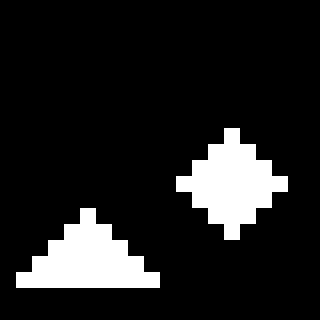
\includegraphics[width=0.6\textwidth]{poly20_zoom}
        \caption{Sample from \textit{poly\_20} (zoom).}
    \end{minipage}
    \hfil
    \begin{minipage}{0.45\textwidth}
        \centering
        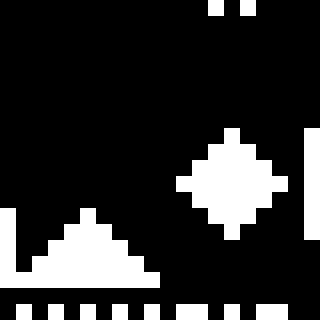
\includegraphics[width=0.6\textwidth]{poly20_pc_zoom}
        \caption{Sample from \textit{poly\_20\_pc} (zoom).}
    \end{minipage}
\end{figure}

The second data set is identical to the first but for the usage of the pixels on the outer border. Each of them now represents a \textit{parity check} of other close inner pixels. In particular, a pixel lying on a vertical border (left or right) will be the parity check of the $9$ inner nearest pixels lying on the same row (left-half or right-half). Similarly, a pixel lying on a horizontal border (top or down) will be the parity check of the $9$ inner nearest pixels lying on the same column (top-half or bottom-half). By assigning the values of $0$ and $1$ to, respectively, black and white pixels, we can formally describe the borders of a matrix-like image $I$:

\begin{equation}
\label{eq:parity_check}
\forall i = 1, ..., 20: 
\begin{cases}
     I[i][0] = \sum\limits_{k=2}^{10} I[i][k] \mod 2 & \text{(bottom-half columns)} \\
     I[i][20] = \sum\limits_{k=11}^{19} I[i][k] \mod 2 & \text{(top-half columns)} \\
     I[0][i] = \sum\limits_{k=2}^{10} I[k][i] \mod 2 & \text{(left-half rows)} \\
     I[20][i] = \sum\limits_{k=11}^{19} I[k][i] \mod 2 & \text{(right-half rows)} \\
\end{cases}.
\end{equation}

The second data set is labelled as \textit{poly20\_pc}.

\begin{figure}[ht]
    \centering
    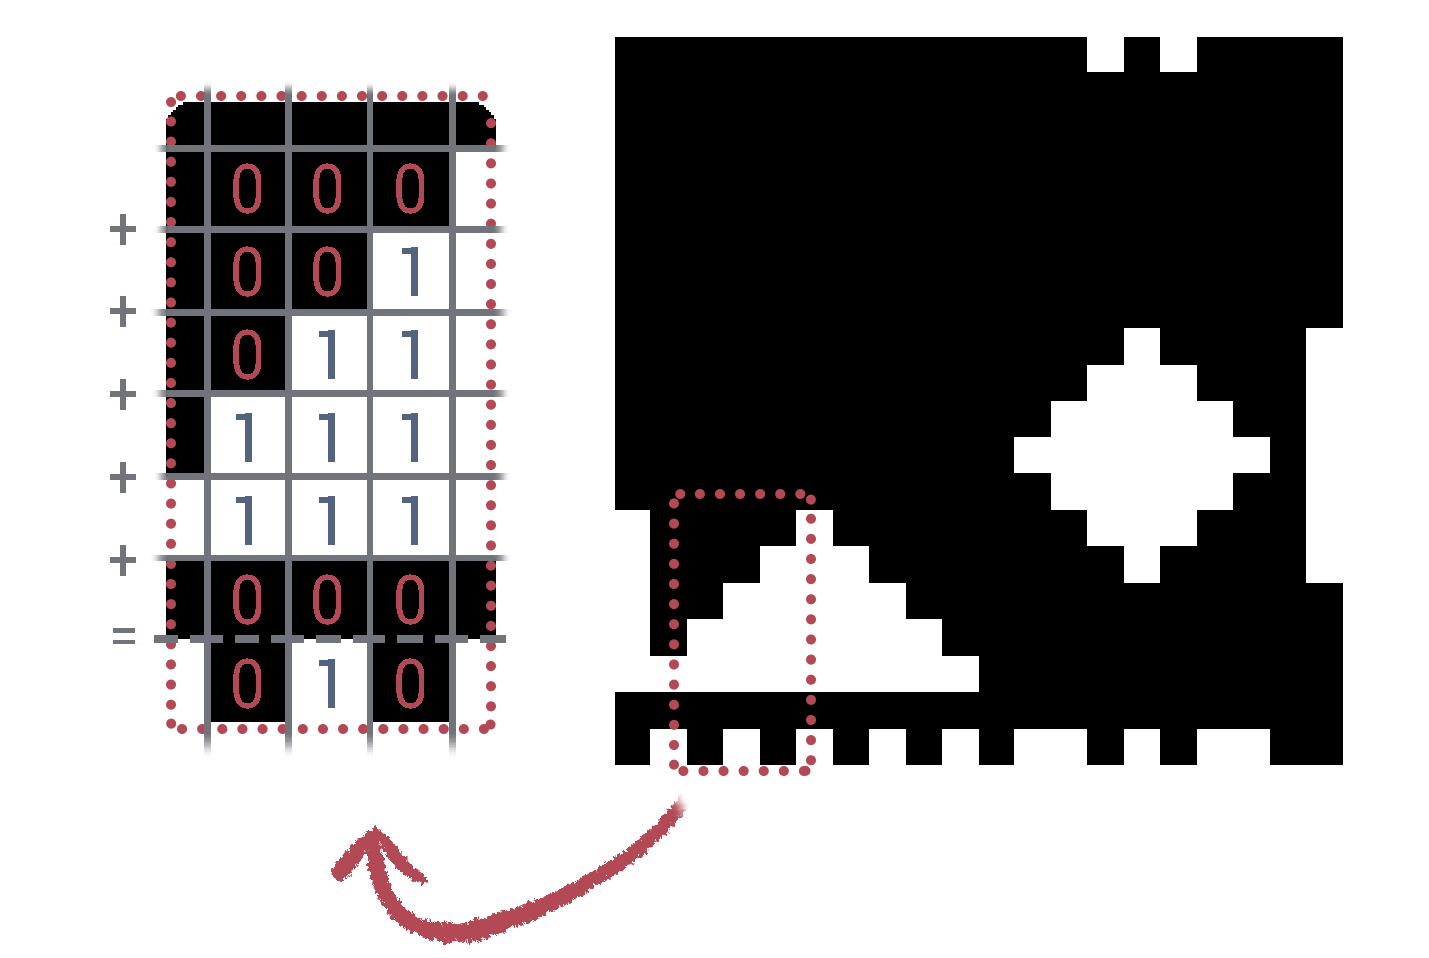
\includegraphics[width=0.7\textwidth]{pc_zoom}
    \caption{Schematic representation of how parity checks are computed.}
\end{figure}

The two data sets have been generated according to the following criteria:

\begin{itemize}
    \item the number of items in the data sets is as large as possible, yet bounded by the constraints on the polygons area and their non-overlapping placement;
    \item small $20$x$20$ pixel images allow a faster training with modest-size ANNs architectures that comes handy in an exploratory research scenario;
    \item placing two polygons on each image, instead of a single one, avoids the \textit{mode collapsing problem} of GANs. In fact, by doing so, the generator can not try to learn only the easiest shape, that is the one more frequently classified as a training datum by the discriminator. Instead, it is continually forced to learn combinations of them and, consequently, each of them. This evidence is the result of some preliminary experiments on GANs;
    \item rhombi are supposed to be the most difficult polygons to learn among the three available, so they are slightly more present in the data sets;
    \item the constant value of $25$ for the polygons area maximises the number of convex regular polygons that can be discretely represented;
    \item each parity check is computed only on one half of the image to model a function of modest complexity. If desired, these constraints can become harder by extending them on entire rows/columns.
\end{itemize}


A final note regards the choice of parity check pixels in \textit{poly20\_pc}. Their goal is to dramatically reduce the probability for the generator to output a perfect object without having first learnt the rules that define the border of the images. Each parity check, in fact, halves the probability to generate by chance a perfect object. In this way, the generator is forced to learn the relations expressed in \eqref{eq:parity_check}. Furthermore, from a computational point of view, checking if a pixel is correct is very fast. Hence, parity checks seem a suitable family of functions to test the proposed deep generative model: functions that are hard to learn and easy to verify.


\section{Model implementation}

The deep generative framework is implemented in Python and will be open-sourced. The input of the software is a JSON file describing the experiment to be run. It contains information about the data set to be generated or reused, the ANNs architectures and some training parameters and hyperparameters. Every descriptor is thus sufficient to train and evaluate the entire model. Experiments are deterministic and reproducible since JSON files also contain the seeds for the random distributions.

ANNs are trained using TensorFlow \cite{tensorflow}, the open-source ML framework developed by Google. The experiment descriptor includes function names to be used to build the model, together with references to the loss function and the optimization algorithm.

The JSON file can optionally contain a list of constraints. If provided, the resulting generative model will be that of CANs, otherwise simple BGANs. In the first case, constraints will be used during training according to the ANN model specified.

To reduce execution times, penalty functions are dynamically compiled to native machine instructions with Numba \cite{numba}   and they are evaluated in parallel on sampled data by all available CPU cores, avoiding Python's Global Interpreter Lock. In addition, generated samples are also independent of each other, so they can be further processed in parallel in a thread-safe way. On the contrary, data sets penalty vectors are computed once, at the beginning of the training algorithm, and cached, since their values never change. As a result, this single-GPU/multi-core implementation provides similar running times for BGANs and CANs.

Statistics are collected during the training mainly via TensorBoard, the native visualization tool tightly integrated with TensorFlow. This is the best solution to get insights on the training process since some parts of the computation are compiled for the GPU and not exposed via any API. Statistics can be collected with a customized frequency both on the validation set and on the test set.


\section{Experimental protocol}


Probabilistic generative models can be used for many different tasks, such as compression, denoising, semi-supervised learning or unsupervised feature learning. Given this wide range of applications, a lot of heterogeneity exists in the way these models are trained and evaluated. Some works have proved that good performance with respect to one criterion do not imply good performance with respect to other criteria \cite{evaluation}. Since being able to generate realistic samples from the data distribution
is one of the goals of a generative model, sometimes they are simply evaluated by visually inspecting the samples. Typically, the evaluation is carried out by experimental subjects who do not know the source of the samples \cite{human_evaluators}. Unfortunately, it is possible for a very poor probabilistic model to produce very good samples. However, the framework of this work enables an objective evaluation via penalty functions and no subjective assessment is necessary.

ANNs generally require a significative amount of random numbers to be trained. They are used, for instance, to initialize the weights of the network or to randomly shuffle mini-batches before every new training epoch. GANs-based models, in particular, involve a far greater amount of noise, since new vectors are required to sample data from $p_g$ and this operation is usually performed a million times. However, due to computational implications, extensively testing ANNs can be really time-consuming and it can be hard to get results with a high significance level.

Experiments have been repeated multiple times with different random seeds. Each plot shows the number of repetitions and highlights the first, second and third quartiles of the aggregated results regarding the performance measure of interest.

Networks have been evaluated for their capability to satisfy constraints individually and simultaneously. In the first case, plots show the average over all constraints of the percentages of objects satisfying each of them. In the latter, they show the percentage of perfect objects produced. In both cases, the images involved in the measurement are those generated during a training epoch on the test set after which no optimization is performed.

The tested BGANs and CANs architectures are equivalent, with the obvious exception of the hidden units reserved for the constraints, that are CANs-specific. Networks are also initialized in the same way and visually evaluated on the same input noise. To measure their capability of generating objects satisfying constraints, a number of statistics are periodically collected during training, such as the percentage of perfect objects being generated or the mean error on each penalty function.

Stochastic optimization is performed via Adam \cite{adam} and batch normalization \cite{batch_norm} is used on some layers to accelerate training.

The reported execution times refer to the experiments performed on \textit{Maximillian Pegasus}\footnote{Lorenzo, thanks from the bottom of my heart.}: CPU Intel Core i$7$-$5930$K $3.5$GHz, $6$ cores; $3$x GPU MSI GeForce GTX $980$, $4$GB; RAM $16$GB; OS Windows $10$; Python version $3.5.2$; TensorFlow-GPU version $1.6.0$; Nvidia driver $391.01$; CUDA version $9.0$; cuDNN version $7.0.5$.


\section{Model architectures}

Not being interested in finding the best architecture for the task, but only in comparing BGANs and CANs with the same architecture, the experimentation does not involve model selection. On the contrary, the architecture initially adopted, together with all its hyperparameters, is the one described in the original work on BGANs. Preliminary works on BGANs have proved this architecture to have enough capacity to learn in a reasonable amount of time how to generate images of different kinds. Similarly to data sets, also architectures are labelled for convenience.

Generators and discriminators tend to have symmetric configurations. This choice makes the adversarial training procedure quite stable over the epochs and overall effective. Discriminator architectures usually involve convolutional layers to learn spatially local patterns of input polygons. Vice versa, generator architectures use the opposite operation, the transposed convolution layer, often simply called deconvolution, to expand input noise into meaningful shapes.

The following is a schematic description of the architectures. For each of them is provided the complete list of composing layers, along with their parameters and input/output dimensions. The symbol $\stackrel{r}{\to}$ is used to indicate reshaping operations. The symbol $\stackrel{t}{\to}$ represents a transpose operation. The symbol $\stackrel{c}{\to}$ denotes that the layer has been expanded to introduce hidden units to be fed with values computed by penalty functions.

The placeholder $?$ is used for input values. For generator architectures usually it is $|\bm{z}| \times |mini\text{-}batch|$, while for discriminator architectures it is $|samples| \times |mini\text{-}batch|$, where $|samples|$ represents the number of samples drawn for each generator output, as specified by BGANs. Default values are $|\bm{z}| = 64$, $|samples| = 20$, $|mini\text{-}batch| = 64$.


\begin{description}
\item \textit{bgan20\_gen}: generator network originally used for BGANs, adapted for 20x20 pixel data sets.
\begin{enumerate}
    \item $(?, 64) \to (?, 1024)$. Type: dense ($1024$ output units); activation: ReLU; batch normalization. 
    \item $(?, 1024) \to (?, 3200)$. Type: dense ($3200$ output units); activation: ReLU; batch normalization.
    \item $(?, 3200) \stackrel{r}{\to} (?, 5, 5, 128) \to (?, 10, 10, 64)$. Type: deconvolution; filters: 64; kernel size: 5; strides: 2; kernel initializer: orthogonal; bias initializer: zeros; activation: ReLU; batch normalization.
    \item $(?, 10, 10, 64) \to (?, 20, 20, 1)$. Type: deconvolution; filters: 1; kernel size: 5; strides: 2; kernel initializer: orthogonal; bias initializer: zeros; activation: linear.
   \end{enumerate}
\item \textit{bgan20\_discr\_h32l}: discriminator network similar to the one originally used for BGANs, adapted for 20x20 pixel data sets. Layer \ref{additional_layer} is added for consistency with the corresponding constrained discriminator layer reserved for penalty function values (\textit{can20\_discr\_h32l}, layer \ref{constrained_layer}).
\begin{enumerate}
    \item $(?, 20, 20, 1) \to (?, 10, 10, 64)$. Type: convolution; filters: 64; kernel size: 5; strides: 2; kernel initializer: Xavier; activation: leaky ReLU ($a = 0.2$).
    \item $(?, 10, 10, 64) \to (?, 5, 5, 128)$. Type: convolution; filters: 128; kernel size: 5; strides: 2; kernel initializer: Xavier; activation: leaky ReLU ($a = 0.2$).
    \item $(?, 5, 5, 128) \stackrel{r}{\to} (?, 3200) \to (?, 1024)$. Type: dense ($1024$ output units); kernel initializer: Xavier; activation: leaky ReLU ($a = 0.2$).
    \item \label{additional_layer} $(?, 1024) \to (?, 32)$. Type: dense ($32$ output units); kernel initializer: Xavier; activation: leaky ReLU ($a = 0.2$).
    \item $(?, 32) \to (?, 1)$. Type: dense ($1$ output unit); kernel initializer: Xavier; activation: linear.
\end{enumerate}

\item \textit{can20\_discr\_h32l}: discriminator layer with constraints introduced before computing the original output, in an intermediate layer. The choice of $32$ hidden units for layer \ref{constrained_layer} is arbitrary.
\begin{enumerate}
    \item $(?, 20, 20, 1) \to (?, 10, 10, 64)$. Type: convolution; filters: 64; kernel size: 5; strides: 2; kernel initializer: Xavier; activation: leaky ReLU ($a = 0.2$).
    \item $(?, 10, 10, 64) \to (?, 5, 5, 128)$. Type: convolution; filters: 128; kernel size: 5; strides: 2; kernel initializer: Xavier; activation: leaky ReLU ($a = 0.2$).
    \item $(?, 5, 5, 128) \stackrel{r}{\to} (?, 3200) \to (?, 1024)$. Type: dense ($1024$ output units); kernel initializer: Xavier; activation: leaky ReLU ($a = 0.2$).
    \item $(?, 1024) \to (?, 32)$. Type: dense ($32$ output units); kernel initializer: Xavier; activation: leaky ReLU ($a = 0.2$).
    \item \label{constrained_layer} \textit{if} $|\mathbb{C}| > 0$: $(?, 32) \stackrel{c}{\to} (?, 32+|\mathbb{C}|)$. Type: dense ($32+|\mathbb{C}|$ output units); kernel initializer: Xavier; bias initializer: Xavier; activation: linear.
    \item $(?, 32+|\mathbb{C}|) \to (?, 1)$. Type: dense ($1$ output unit); kernel initializer: Xavier; bias initializer: Xavier; activation: linear.
\end{enumerate}

\begin{figure}[ht]
    \centering
    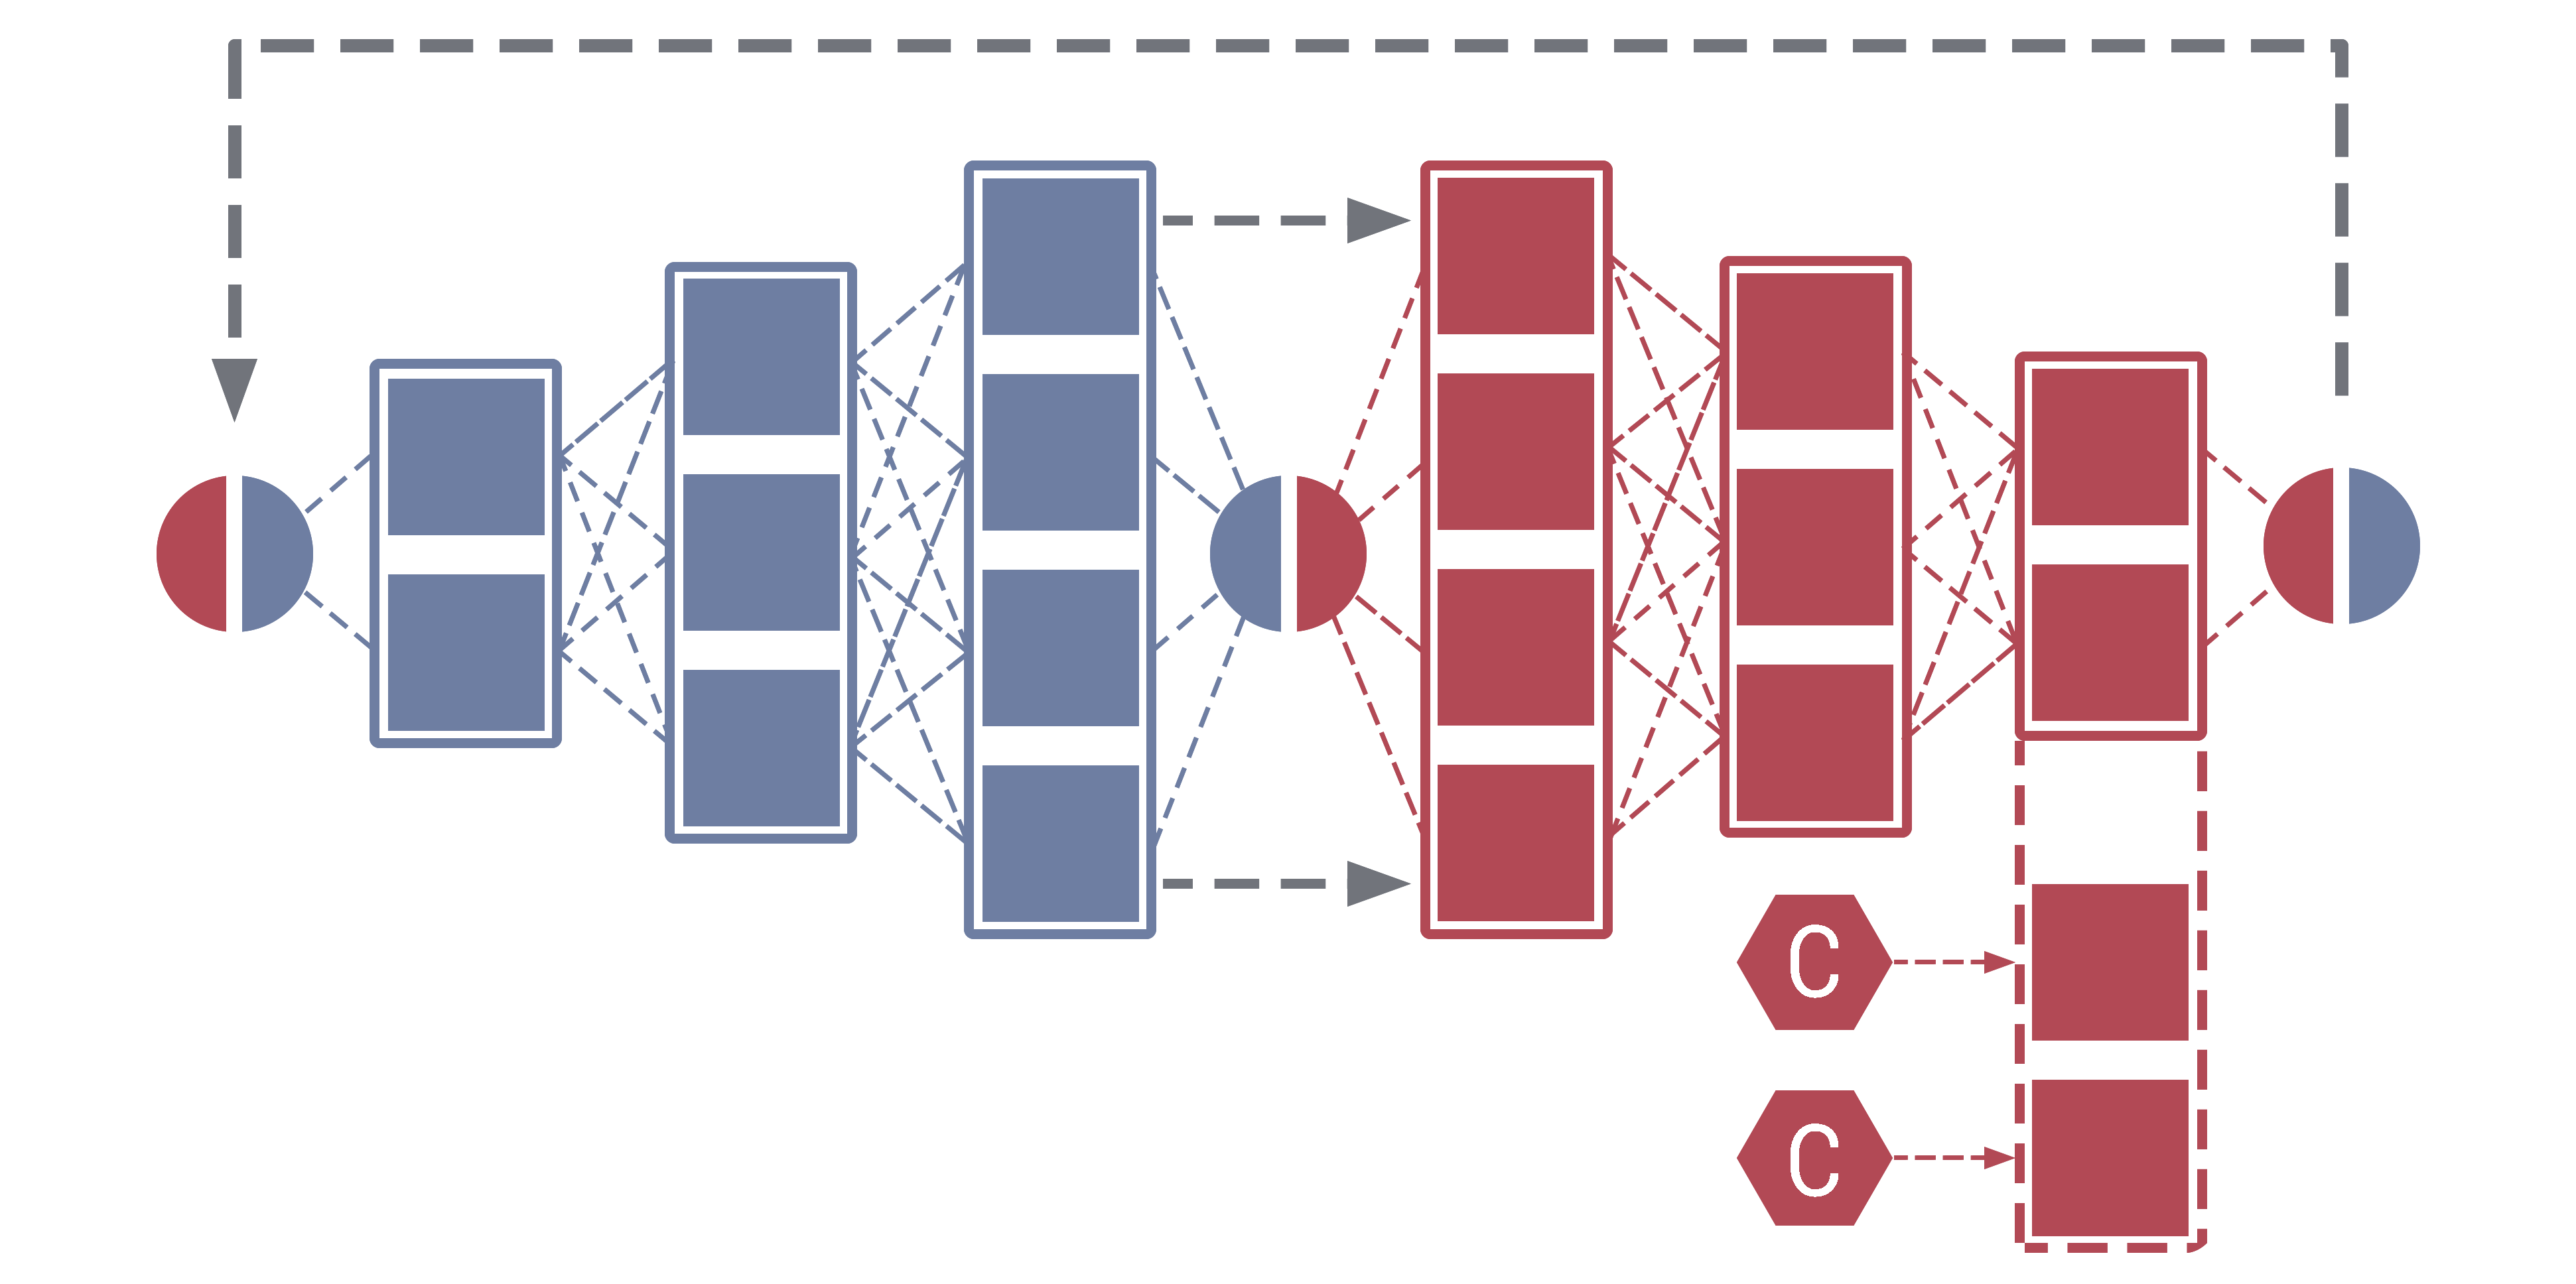
\includegraphics[width=0.7\textwidth]{can20_discr_h32l_schema}
    \caption{Schematic representation of CANs with \textit{can20\_discr\_h32l}. Constraints are introduced in the discriminator (red) in the final hidden layer.}
\end{figure}

\item \textit{can20\_discr\_outl}: discriminator layer with constraints introduced after computing the original output, in an additional final layer.
\begin{enumerate}
    \item $(?, 20, 20, 1) \to (?, 10, 10, 64)$. Type: convolution; filters: 64; kernel size: 5; strides: 2; kernel initializer: Xavier; activation: leaky ReLU ($a = 0.2$).
    \item $(?, 10, 10, 64) \to (?, 5, 5, 128)$. Type: convolution; filters: 128; kernel size: 5; strides: 2; kernel initializer: Xavier; activation: leaky ReLU ($a = 0.2$).
    \item $(?, 5, 5, 128) \stackrel{r}{\to} (?, 3200) \to (?, 1024)$. Type: dense ($1024$ output units); kernel initializer: Xavier; activation: leaky ReLU ($a = 0.2$).
    \item $(?, 1024) \to (?, 1)$. Type: dense ($1$ output units); kernel initializer: Xavier; activation: leaky ReLU ($a = 0.2$).
    \item \textit{if} $|\mathbb{C}| > 0$: $(?, |\mathbb{C}|) \stackrel{c}{\to} (?, 1)$. Type: dense ($1$ output unit); kernel initializer: Xavier; activation: linear.
    \item \textit{if} $|\mathbb{C}| > 0$: $(?, 1) \stackrel{c}{\to} (?, 2) \to (?, 1)$. Type: dense ($1$ output unit); kernel initializer: Xavier; bias initializer: Xavier; activation: linear.
\end{enumerate}

\begin{figure}[ht]
    \centering
    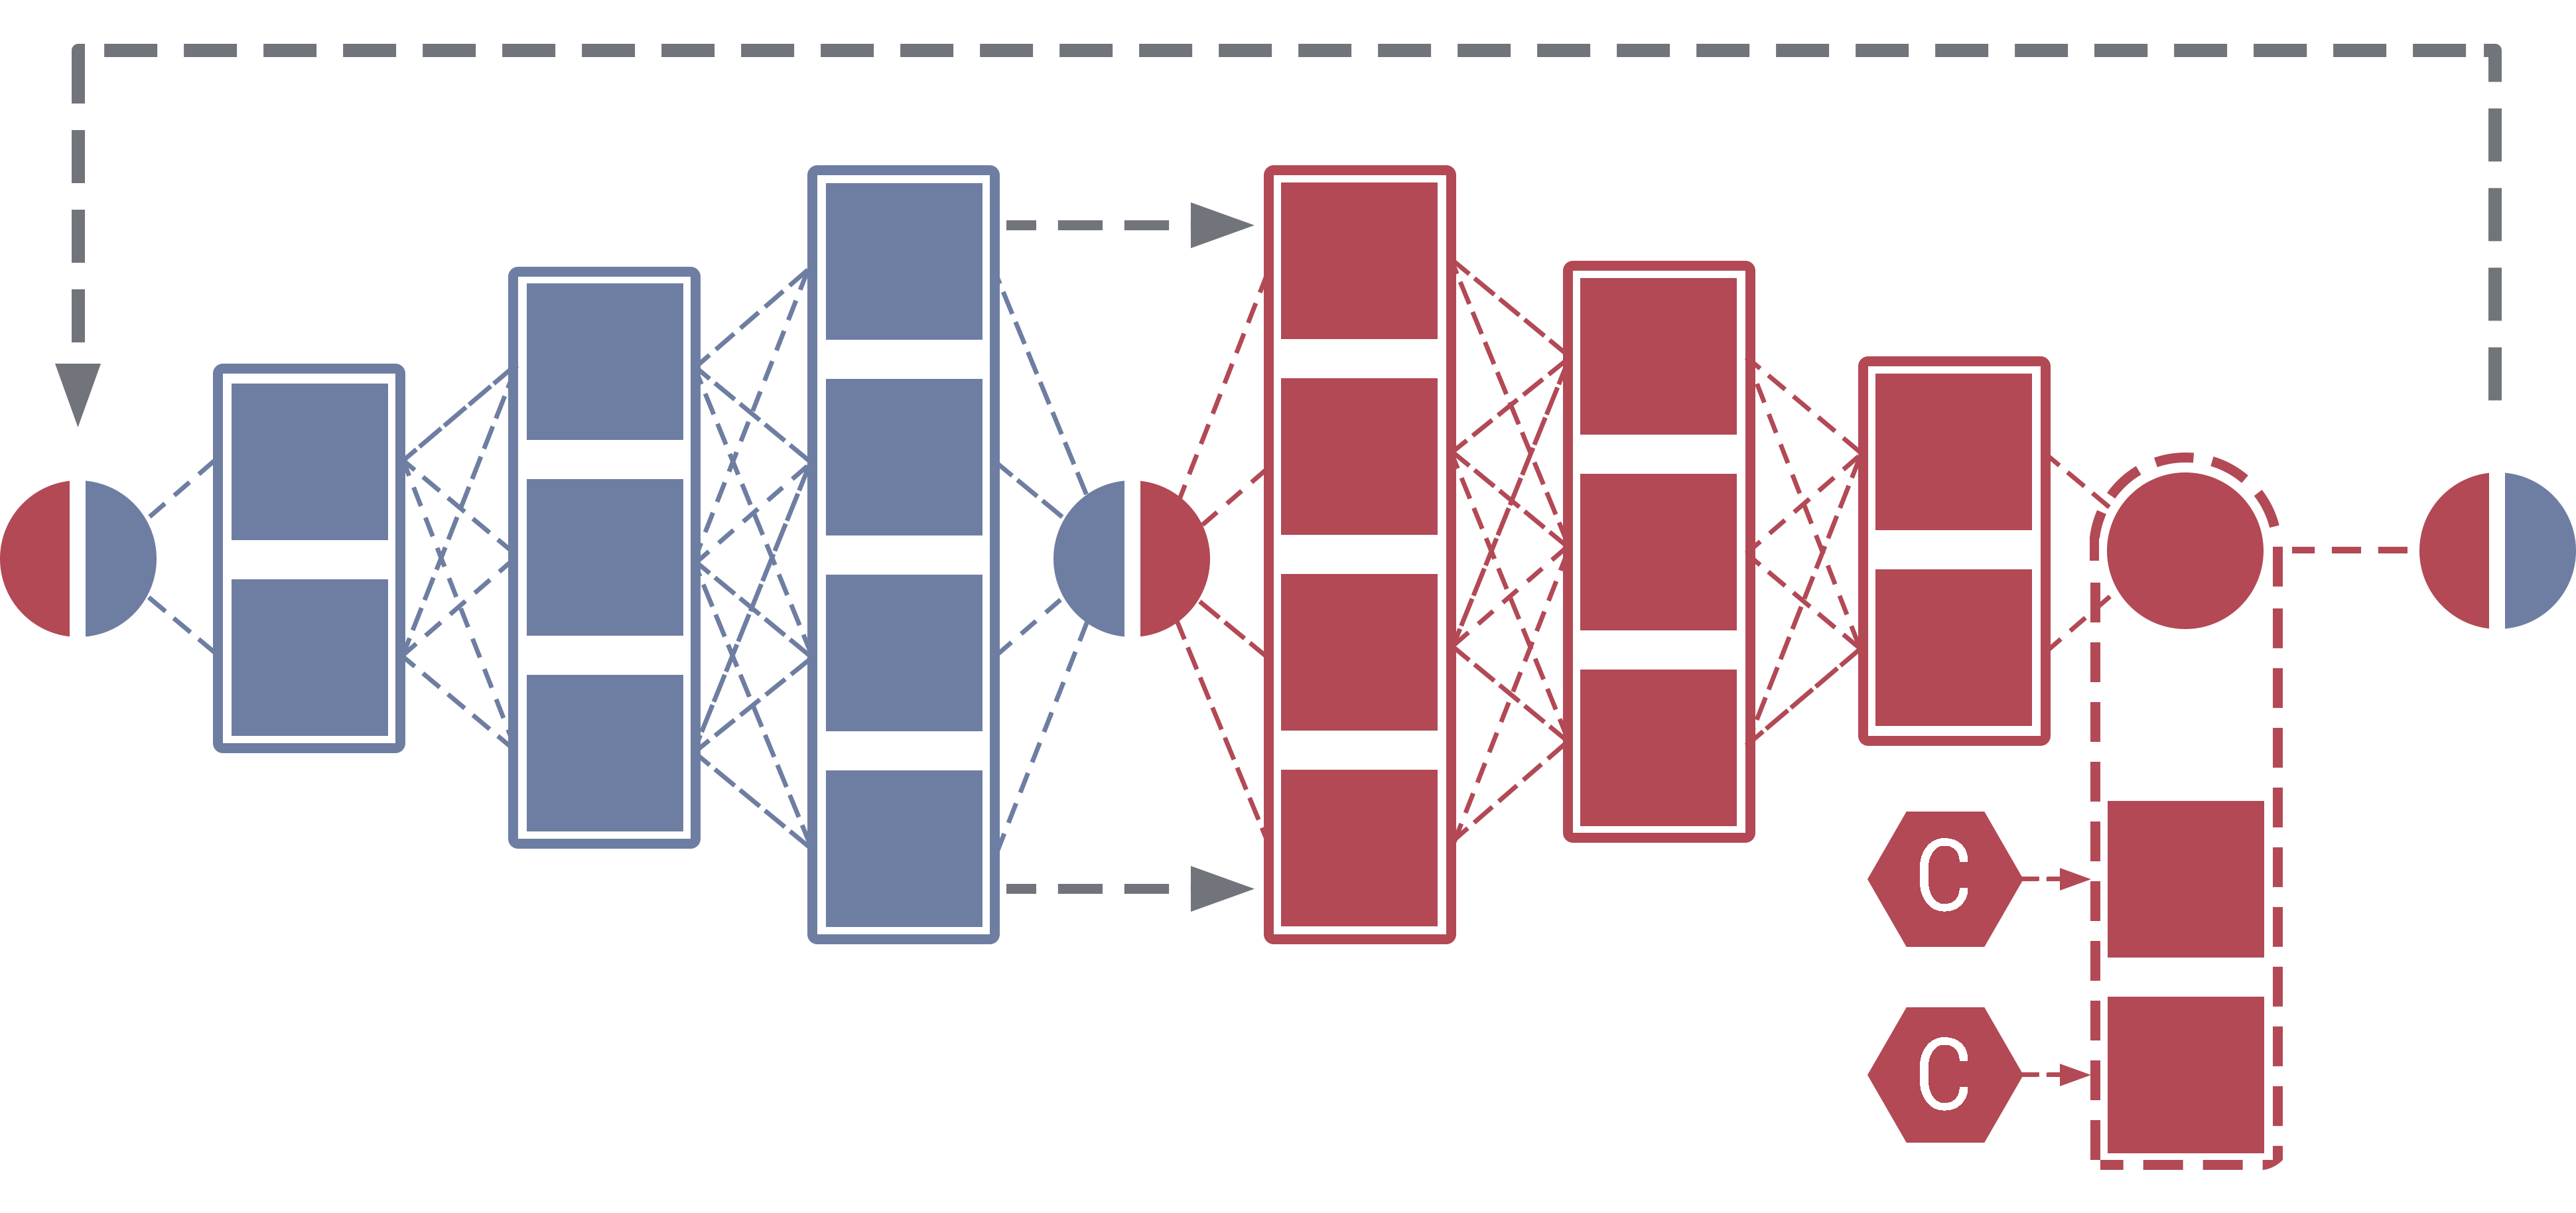
\includegraphics[width=0.7\textwidth]{can20_discr_outl_schema}
    \caption{Schematic representation of CANs with \textit{can20\_discr\_outl}. Constraints are introduced in the discriminator (red) after the final hidden layer.}
\end{figure}

% \item \textit{bgan60\_gen}: generator network originally used for BGANs, adapted for 60x60 pixel data sets. It contains an additional deconvolutional layer (\ref{additional_deconvolution}) to increase model capacity.
% \begin{enumerate}
%     \item $(?, 64) \to (?, 1024)$. Type: dense ($1024$ output units); activation: ReLU; batch normalization. 
%     \item $(?, 1024) \to (?, 3200)$. Type: dense ($3200$ output units); activation: ReLU; batch normalization.
%     \item $(?, 3200) \stackrel{r}{\to} (?, 5, 5, 128) \to (?, 10, 10, 64)$. Type: deconvolution; filters: 64; kernel size: 5; strides: 2; kernel initializer: orthogonal; bias initializer: zeros; activation: ReLU; batch normalization.
%     \item \label{additional_deconvolution} $(?, 10, 10, 64) \to (?, 20, 20, 64)$. Type: deconvolution; filters: 64; kernel size: 5; strides: 2; kernel initializer: orthogonal; bias initializer: zeros; activation: ReLU; batch normalization.
%     \item $(?, 20, 20, 64) \to (?, 60, 60, 1)$. Type: deconvolution; filters: 1; kernel size: 5; strides: 3; kernel initializer: orthogonal; bias initializer: zeros; activation: linear.
%    \end{enumerate}
% 
% \item \textit{can60\_discr\_h32l}: discriminator network originally used for BGANs, adapted for 60x60 pixel data sets. It contains an additional convolutional layer (\ref{additional_convolution}) to increase model capacity.
% \begin{enumerate}
%     \item $(?, 60, 60, 1) \to (?, 30, 30, 64)$. Type: convolution; filters: 64; kernel size: 5; strides: 2; kernel initializer: Xavier; activation: leaky ReLU ($a = 0.2$).
%     \item \label{additional_convolution} $(?, 30, 30, 64) \to (?, 15, 15, 64)$. Type: convolution; filters: 64; kernel size: 5; strides: 2; kernel initializer: Xavier; activation: leaky ReLU ($a = 0.2$).
%     \item $(?, 15, 15, 64) \to (?, 8, 8, 128)$. Type: convolution; filters: 128; kernel size: 5; strides: 2; kernel initializer: Xavier; activation: leaky ReLU ($a = 0.2$).
%     \item $(?, 8, 8, 128) \stackrel{r}{\to} (?, 8192) \to (?, 1024)$. Type: dense ($1024$ output units); kernel initializer: Xavier; activation: leaky ReLU ($a = 0.2$).
%     \item $(?, 1024) \to (?, 32)$. Type: dense ($32$ output units); kernel initializer: Xavier; activation: leaky ReLU ($a = 0.2$).
%     \item \textit{if} $|\mathbb{C}| > 0$: $(?, 32) \stackrel{c}{\to} (?, 32+|\mathbb{C}|)$. Type: dense ($32+|\mathbb{C}|$ output units); kernel initializer: Xavier; bias initializer: Xavier; activation: linear.
%     \item $(?, 32+|\mathbb{C}|) \to (?, 1)$. Type: dense ($1$ output unit); kernel initializer: Xavier; bias initializer: Xavier; activation: linear.
% \end{enumerate}
\end{description}


\section{Penalty functions}

According to the criteria by which data sets \textit{poly20} and \textit{poly20\_pc} have been generated, it is possible to define some constraints on the images. The following is a schematic list, with their corresponding penalty functions and labels.


\begin{description}
\item \textit{smaller\_area}: require the image to not contain less than the expected number of white pixels ($2\times25$). The penalty is proportional to the underestimation.
\begin{enumerate}
\item[] $f(I): min(1, max(0, 2\cdot25 - \sum\limits_{i=1}^{20} \sum\limits_{j=1}^{20} M[i][j]) / (20\cdot20 - 2\cdot25))$
\end{enumerate}

\item \textit{greater\_area}: require the image to not contain more than the expected number of white pixels ($2\times25$). The penalty is proportional to the overestimation.
\begin{enumerate}
\item[] $f(I): min(1, max(0, - 2\cdot25 + \sum\limits_{i=1}^{20} \sum\limits_{j=1}^{20} M[i][j]) / (20\cdot20 - 2\cdot25))$
\end{enumerate}

\item \textit{convex}: require the image to only contain convex shapes. The penalty is proportional to the number of pixels contained in concave zones defined by polygons. Shapes are identified with a breadth-first search in a graph representing the image. Wrong pixels are detected scanning the image by rows, columns and diagonals.
\begin{enumerate}
\item[] $f(I): min(1, (\sum\limits_{i=1}^{20} \sum\limits_{j=1}^{20} M[i][j] \text{ if in concave zone}) / (2\cdot20\cdot20))$
\end{enumerate}

\item \textit{parity\_check\_p\_i}: require the image to correctly set a parity check pixel on the border. The placeholder $p$ can be one of \{rl, rr, ct, cb\} to indicate that the $i\text{-}th$ pixel involves, respectively, a left-half row, a right-half row, a top-half column or a bottom-half column. The penalty assigned is binary: $0$ if the relation \ref{eq:parity_check} is true for the $i\text{-}th$ pixel, $1$ otherwise.

\end{description}


All the penalty functions can be straightforwardly extended to data sets of larger images or with a different number of polygons.

Since experiments have been performed reusing the same sets of penalty functions, additional labels are also provided for them (range notation adopted for conciseness):

\begin{description}
\item \textit{area\_convex}: $\mathbb{C} = \{\textit{smaller\_area, greater\_area, convex}\}$, $|\mathbb{C}| = 3$.

\item \textit{some\_pc}: $\mathbb{C} = \{\textit{smaller\_area, greater\_area, parity\_check\_rl\_1-9, parity\_check\_ct\_1-9}\}$, $|\mathbb{C}| = 20$.

\item \textit{all\_pc}: $\mathbb{C} = \{\textit{smaller\_area, greater\_area, parity\_check\_rl-ct-rr-cb\_1-18}\}$, $|\mathbb{C}| = 74$.
\end{description}



\section{Experiments}

The goal of the first experiment is to compare BGANs and CANs with the simplest data set, \textit{poly20}, and a small set of constraints, \textit{area\_convex}. 
Figures \ref{fig:D_poly20_C_area_convex_N_bgan_can_perfect} and \ref{fig:D_poly20_C_area_convex_N_bgan_can_avg_constraints_satisfaction} show that BGANs are superior to CANs both for the percentage of perfect objects generated and for average constraints satisfaction. The reason is probably related to the constraints involved, that are uninformative and insufficient to better guide the generator in the search space for CANs while introducing additional parameters that unnecessarily burden the training. This evidence justifies the use of the other data set, \textit{poly20\_pc}, and more informative penalty functions.

\begin{figure}[ht]
    \centering
    \begin{minipage}[t]{0.45\textwidth}
        \centering
        \includegraphics[width=\textwidth]{D_poly20_C_area_convex_N_bgan_can_perfect}
        \caption{\\BGANs: \textit{bgan20\_gen} + \textit{bgan20\_discr\_h32l}.\\
        CANs: \textit{bgan20\_gen} + \textit{can20\_discr\_h32l}.}
        \label{fig:D_poly20_C_area_convex_N_bgan_can_perfect}
    \end{minipage}
    \hfill
    \begin{minipage}[t]{0.45\textwidth}
        \centering
        \includegraphics[width=\textwidth]{D_poly20_C_area_convex_N_bgan_can_avg_constraints_satisfaction}
        \caption{\\BGANs: \textit{bgan20\_gen} + \textit{bgan20\_discr\_h32l}.\\
        CANs: \textit{bgan20\_gen} + \textit{can20\_discr\_h32l}.}
        \label{fig:D_poly20_C_area_convex_N_bgan_can_avg_constraints_satisfaction}
    \end{minipage}
\end{figure}


Opposite results are observed when the data distribution to be learnt is harder, such as for \textit{poly20\_pc}. In this case, CANs benefit from the constraints expressed in \textit{some\_pc} and achieve better performance than BGANs, as depicted in figures \ref{fig:D_poly20_pc_C_some_pc_N_bgan_can_perfect} and \ref{fig:D_poly20_pc_C_some_pc_N_bgan_can_avg_constraints_satisfaction}.

\begin{figure}[ht]
    \centering
    \begin{minipage}[t]{0.45\textwidth}
        \centering
        \includegraphics[width=\textwidth]{D_poly20_pc_C_some_pc_N_bgan_can_perfect}
        \caption{\\BGANs: \textit{bgan20\_gen} + \textit{bgan20\_discr\_h32l}.\\
        CANs: \textit{bgan20\_gen} + \textit{can20\_discr\_h32l}.}
        \label{fig:D_poly20_pc_C_some_pc_N_bgan_can_perfect}
    \end{minipage}
    \hfill
    \begin{minipage}[t]{0.45\textwidth}
        \centering
        \includegraphics[width=\textwidth]{D_poly20_pc_C_some_pc_N_bgan_can_avg_constraints_satisfaction}
        \caption{\\BGANs: \textit{bgan20\_gen} + \textit{bgan20\_discr\_h32l}.\\
        CANs: \textit{bgan20\_gen} + \textit{can20\_discr\_h32l}.}
        \label{fig:D_poly20_pc_C_some_pc_N_bgan_can_avg_constraints_satisfaction}
    \end{minipage}
\end{figure}

The differences between the two models are nevertheless small, with the biggest improvement observed in average constraints satisfaction. Figure \ref{fig:D_poly20_pc_C_some_pc_N_bgan_can_avg_constraints_satisfaction_delta} shows that the gap between BGANs and CANs tends to disappear as training continues. This result is reasonable, since BGANs are provided with enough capacity to learn the correct distribution anyway. Nevertheless, it can be considered significative because CANs only require small additional time to be trained, as demonstrated in figure \ref{fig:D_poly20_pc_C_some_pc_N_bgan_can_time}.

\begin{figure}[ht]
    \centering
    \begin{minipage}[t]{0.45\textwidth}
        \centering
        \includegraphics[width=\textwidth]{D_poly20_pc_C_some_pc_N_bgan_can_avg_constraints_satisfaction_delta}
        \caption{\\BGANs: \textit{bgan20\_gen} + \textit{bgan20\_discr\_h32l}.\\
        CANs: \textit{bgan20\_gen} + \textit{can20\_discr\_h32l}.}
        \label{fig:D_poly20_pc_C_some_pc_N_bgan_can_avg_constraints_satisfaction_delta}
    \end{minipage}
    \hfill
    \begin{minipage}[t]{0.45\textwidth}
        \centering
        \includegraphics[width=\textwidth]{D_poly20_pc_C_some_pc_N_bgan_can_time}
        \caption{\\BGANs: \textit{bgan20\_gen} + \textit{bgan20\_discr\_h32l}.\\CANs: \textit{bgan20\_gen} + \textit{can20\_discr\_h32l}.}
        \label{fig:D_poly20_pc_C_some_pc_N_bgan_can_time}
    \end{minipage}
\end{figure}


Some insights can be drawn when comparing two CANs, one using constraints on the last hidden layer and the other on the output layer. Figure \ref{fig:D_poly20_pc_C_some_pc_N_can_canout_perfect} shows how the first architecture is more effective in learning each single constraint in the long term, producing many more perfect objects. On the other side, figure \ref{fig:D_poly20_pc_C_some_pc_N_can_canout_avg_constraints_satisfaction} suggests that modelling the discriminator's output and the constraints as having the same relevance may largely impact the average number of constraints satisfied at the beginning of the training procedure. This trade-off deserves further research in future work.

\begin{figure}[ht]
    \centering
    \begin{minipage}[t]{0.45\textwidth}
        \centering
        \includegraphics[width=\textwidth]{D_poly20_pc_C_some_pc_N_can_canout_perfect}
        \caption{\\CANs: \textit{bgan20\_gen} + \textit{can20\_discr\_h32l}.\\
        CANs\_out: \textit{bgan20\_gen} + \textit{can20\_discr\_outl}.}
        \label{fig:D_poly20_pc_C_some_pc_N_can_canout_perfect}
    \end{minipage}
    \hfill
    \begin{minipage}[t]{0.45\textwidth}
        \centering
        \includegraphics[width=\textwidth]{D_poly20_pc_C_some_pc_N_can_canout_avg_constraints_satisfaction}
        \caption{\\CANs: \textit{bgan20\_gen} + \textit{can20\_discr\_h32l}.\\
        CANs\_out: \textit{bgan20\_gen} + \textit{can20\_discr\_outl}.}
        \label{fig:D_poly20_pc_C_some_pc_N_can_canout_avg_constraints_satisfaction}
    \end{minipage}
\end{figure}


In all the experiments presented so far using the set of constraints \textit{some\_pc} it is evident that networks achieve excellent performances in satisfying each constraint on average ($95\%+$), but not in generating perfect objects (${\sim}65\%$). The same experiments have also been conducted using a double amount of training epochs. Figure \ref{fig:D_poly20_pc_C_some_pc_N_bgan_can_bganlong_canlong_perfect} shows that, on longer runs, not only the number of perfect objects increases over epochs, but the gap between BGANs and CANs is also preserved.


The ratio behind using only a subset of available parity checks as constraints is that network capable of satisfying some of them should in principle be able to satisfy all of them. This hypothesis is tested by using the complete set of constraints, \textit{all\_pc}.

Figure \ref{fig:D_poly20_pc_C_all_pc_N_bgan_can_perfect} reports the results achieved with a set up equal to that of figure \ref{fig:D_poly20_pc_C_some_pc_N_bgan_can_perfect} but for the usage of the extended constraints set. As expected, both the models now require more training epochs before being able to generate perfect objects (at least $50$). A more interesting observation regards the same performance measured at the end of the training algorithm. It is possible to notice that CANs succeed in generating objects satisfying the two set of constraints with approximately the same probability, while BGANs suffer a great performance loss. The result is better highlighted in figure \ref{fig:D_poly20_pc_C_all_pc_N_bgan_can_perfect_delta}, where a remarkable gap of $16\%$ can be observed between the two architectures at the hundredth epoch.

\begin{figure}[ht]
    \centering
    \begin{minipage}[t]{0.45\textwidth}
        \centering
        \includegraphics[width=\textwidth]{D_poly20_pc_C_some_pc_N_bgan_can_bganlong_canlong_perfect}
        \caption{\\BGANs: \textit{bgan20\_gen} + \textit{bgan20\_discr\_h32l}.\\
        CANs: \textit{bgan20\_gen} + \textit{can20\_discr\_h32l}.\\
        BGANs\_long = BGANs\\
        CANs\_long = CANs.}
        \label{fig:D_poly20_pc_C_some_pc_N_bgan_can_bganlong_canlong_perfect}
    \end{minipage}
    \hfill
    \begin{minipage}[t]{0.45\textwidth}
        \centering
        \includegraphics[width=\textwidth]{D_poly20_pc_C_all_pc_N_bgan_can_perfect}
        \caption{\\BGANs: \textit{bgan20\_gen} + \textit{bgan20\_discr\_h32l}.\\
        CANs: \textit{bgan20\_gen} + \textit{can20\_discr\_h32l}.}
        \label{fig:D_poly20_pc_C_all_pc_N_bgan_can_perfect}
    \end{minipage}
\end{figure}

It is worth noting that, due to the kind of constraints involved and to the multi-core implementation, the difference in execution times remains small, as reported in figure \ref{fig:D_poly20_pc_C_all_pc_N_bgan_can_time}. This proves that the model is able to scale and to learn how to satisfy constraints in polynomial-time if penalty functions can be evaluated in polynomial-time as well. Results regarding average constraints satisfaction are similar to the previous ones and thus omitted.

\begin{figure}[ht]
    \centering
    \begin{minipage}[t]{0.45\textwidth}
        \centering
        \includegraphics[width=\textwidth]{D_poly20_pc_C_all_pc_N_bgan_can_perfect_delta}
        \caption{\\BGANs: \textit{bgan20\_gen} + \textit{bgan20\_discr\_h32l}.\\
        CANs: \textit{bgan20\_gen} + \textit{can20\_discr\_h32l}.}
        \label{fig:D_poly20_pc_C_all_pc_N_bgan_can_perfect_delta}
    \end{minipage}
    \hfill
    \begin{minipage}[t]{0.45\textwidth}
        \centering
        \includegraphics[width=\textwidth]{D_poly20_pc_C_all_pc_N_bgan_can_time}
        \caption{\\BGANs: \textit{bgan20\_gen} + \textit{bgan20\_discr\_h32l}.\\
        CANs: \textit{bgan20\_gen} + \textit{can20\_discr\_h32l}.}
        \label{fig:D_poly20_pc_C_all_pc_N_bgan_can_time}
    \end{minipage}
\end{figure}

% \todor{Another important aspect that must still be evaluated involves the moment in which constraints should be introduced in the training procedure, as discussed in \ref{subsec:constraints_timing}. Many different preliminary experiments have been performed in order to detect automatically the optimal epoch, relying on statistics progressively collected on a validation set. No significant evidence arises from these experiments, so they are omitted for brevity. For the sake of completeness, however, figures \ref{fig:D_poly20_pc_C_all_pc_N_bgan_can_canout_candelay_avg_constraints_satisfaction} and \ref{fig:D_poly20_pc_C_all_pc_N_bgan_can_canout_candelay_perfect} report the results obtained in the same configuration of the previous experiment on other architectures. It is clear that dynamically introducing constraints in a later training phase (e.g. at epoch $100$) does not help the generator. The idea to first let the model learn global properties of objects and then refine its knowledge by introducing constraints thus seems not effective. An informal explanation may be that the generator has already learnt how to model $p_{data}$ and introducing constraints in the adversarial training only causes an imbalance that would force him to forget and re-learn. Additional experiments may explore this research question.}{Abbiamo troppi pochi risultati per fare queste considerazioni, io toglierei discussione e grafici}
% 
% \begin{figure}[ht]
%     \centering
%     \begin{minipage}[t]{0.45\textwidth}
%         \centering
%         \includegraphics[width=\textwidth]{D_poly20_pc_C_all_pc_N_bgan_can_canout_candelay_avg_constraints_satisfaction}
%         \caption{\\BGANs: \textit{bgan20\_gen} + \textit{bgan20\_discr\_h32l}.\\
%         CANs: \textit{bgan20\_gen} + \textit{can20\_discr\_h32l}.\\
%         CANs\_out: \textit{bgan20\_gen} + \textit{can20\_discr\_outl}.\\
%         CANs\_e100 = CANs.\\
%         Constraints are used in CANs\_e100 only from epoch $100$.}
%         \label{fig:D_poly20_pc_C_all_pc_N_bgan_can_canout_candelay_avg_constraints_satisfaction}
%     \end{minipage}
%     \hfill
%     \begin{minipage}[t]{0.45\textwidth}
%         \centering
%         \includegraphics[width=\textwidth]{D_poly20_pc_C_all_pc_N_bgan_can_canout_candelay_perfect}
%         \caption{\\BGANs: \textit{bgan20\_gen} + \textit{bgan20\_discr\_h32l}.\\
%         CANs: \textit{bgan20\_gen} + \textit{can20\_discr\_h32l}.\\
%         CANs\_out: \textit{bgan20\_gen} + \textit{can20\_discr\_outl}.\\
%         CANs\_e100 = CANs.\\
%         Constraints are used in CANs\_e100 only from epoch $100$.}
%         \label{fig:D_poly20_pc_C_all_pc_N_bgan_can_canout_candelay_perfect}
%     \end{minipage}
% \end{figure}


In all the results presented so far CANs appear to improve the BGANs baseline when they have early access to constraints and when penalty functions can be effectively used to guide the network in the search space. However, none of the experiments has evaluated the impact of the size of the data set. To estimate the impact of the number of training examples on the model performance a new smaller data set, \textit{poly20\_pc\_small}, is used. It contains one half of the training examples of \textit{poly20\_pc}, thus being composed of $13,568$ images ($9,472$ for training, $4,096$ for testing).

Results on the same experimental set up are reported in figures \ref{fig:D_poly20_pc_small_C_all_pc_N_bgan_can_avg_constraints_satisfaction} and \ref{fig:D_poly20_pc_small_C_all_pc_N_bgan_can_perfect}. With the smaller data set the gap between CANs and BGANs increases considerably according both to average constraints satisfaction and to the number of perfect objects generated. In this configuration constraints are the most effective and CANs score an improvement superior to $20\%$ to their counterpart, as highlighted in figure  \ref{fig:D_poly20_pc_small_C_all_pc_N_bgan_can_perfect_delta}.

\begin{figure}[ht]
    \centering
    \begin{minipage}[t]{0.45\textwidth}
        \centering
        \includegraphics[width=\textwidth]{D_poly20_pc_small_C_all_pc_N_bgan_can_avg_constraints_satisfaction}
        \caption{\\BGANs: \textit{bgan20\_gen} + \textit{bgan20\_discr\_h32l}.\\
        CANs: \textit{bgan20\_gen} + \textit{can20\_discr\_h32l}.}
        \label{fig:D_poly20_pc_small_C_all_pc_N_bgan_can_avg_constraints_satisfaction}
    \end{minipage}
    \hfill
    \begin{minipage}[t]{0.45\textwidth}
        \centering
        \includegraphics[width=\textwidth]{D_poly20_pc_small_C_all_pc_N_bgan_can_perfect}
        \caption{\\BGANs: \textit{bgan20\_gen} + \textit{bgan20\_discr\_h32l}.\\
        CANs: \textit{bgan20\_gen} + \textit{can20\_discr\_h32l}.}
        \label{fig:D_poly20_pc_small_C_all_pc_N_bgan_can_perfect}
    \end{minipage}
\end{figure}

\begin{figure}[ht]
    \centering
    \begin{minipage}[t]{0.45\textwidth}
        \centering
        \includegraphics[width=\textwidth]{D_poly20_pc_small_C_all_pc_N_bgan_can_perfect_delta}
        \caption{\\BGANs: \textit{bgan20\_gen} + \textit{bgan20\_discr\_h32l}.\\
        CANs: \textit{bgan20\_gen} + \textit{can20\_discr\_h32l}.}
        \label{fig:D_poly20_pc_small_C_all_pc_N_bgan_can_perfect_delta}
    \end{minipage}
    \hfill
    \begin{minipage}[t]{0.45\textwidth}
        \centering
        \includegraphics[width=\textwidth]{D_poly20_pc_small_C_all_pc_N_bgan_can_avg_constraints_satisfaction_delta}
        \caption{\\BGANs: \textit{bgan20\_gen} + \textit{bgan20\_discr\_h32l}.\\
        CANs: \textit{bgan20\_gen} + \textit{can20\_discr\_h32l}.}
        \label{fig:D_poly20_pc_small_C_all_pc_N_bgan_can_avg_constraints_satisfaction_delta}
    \end{minipage}
\end{figure}


\begin{figure}[ht]
    \centering
    \begin{minipage}{0.32\textwidth}
        \centering
        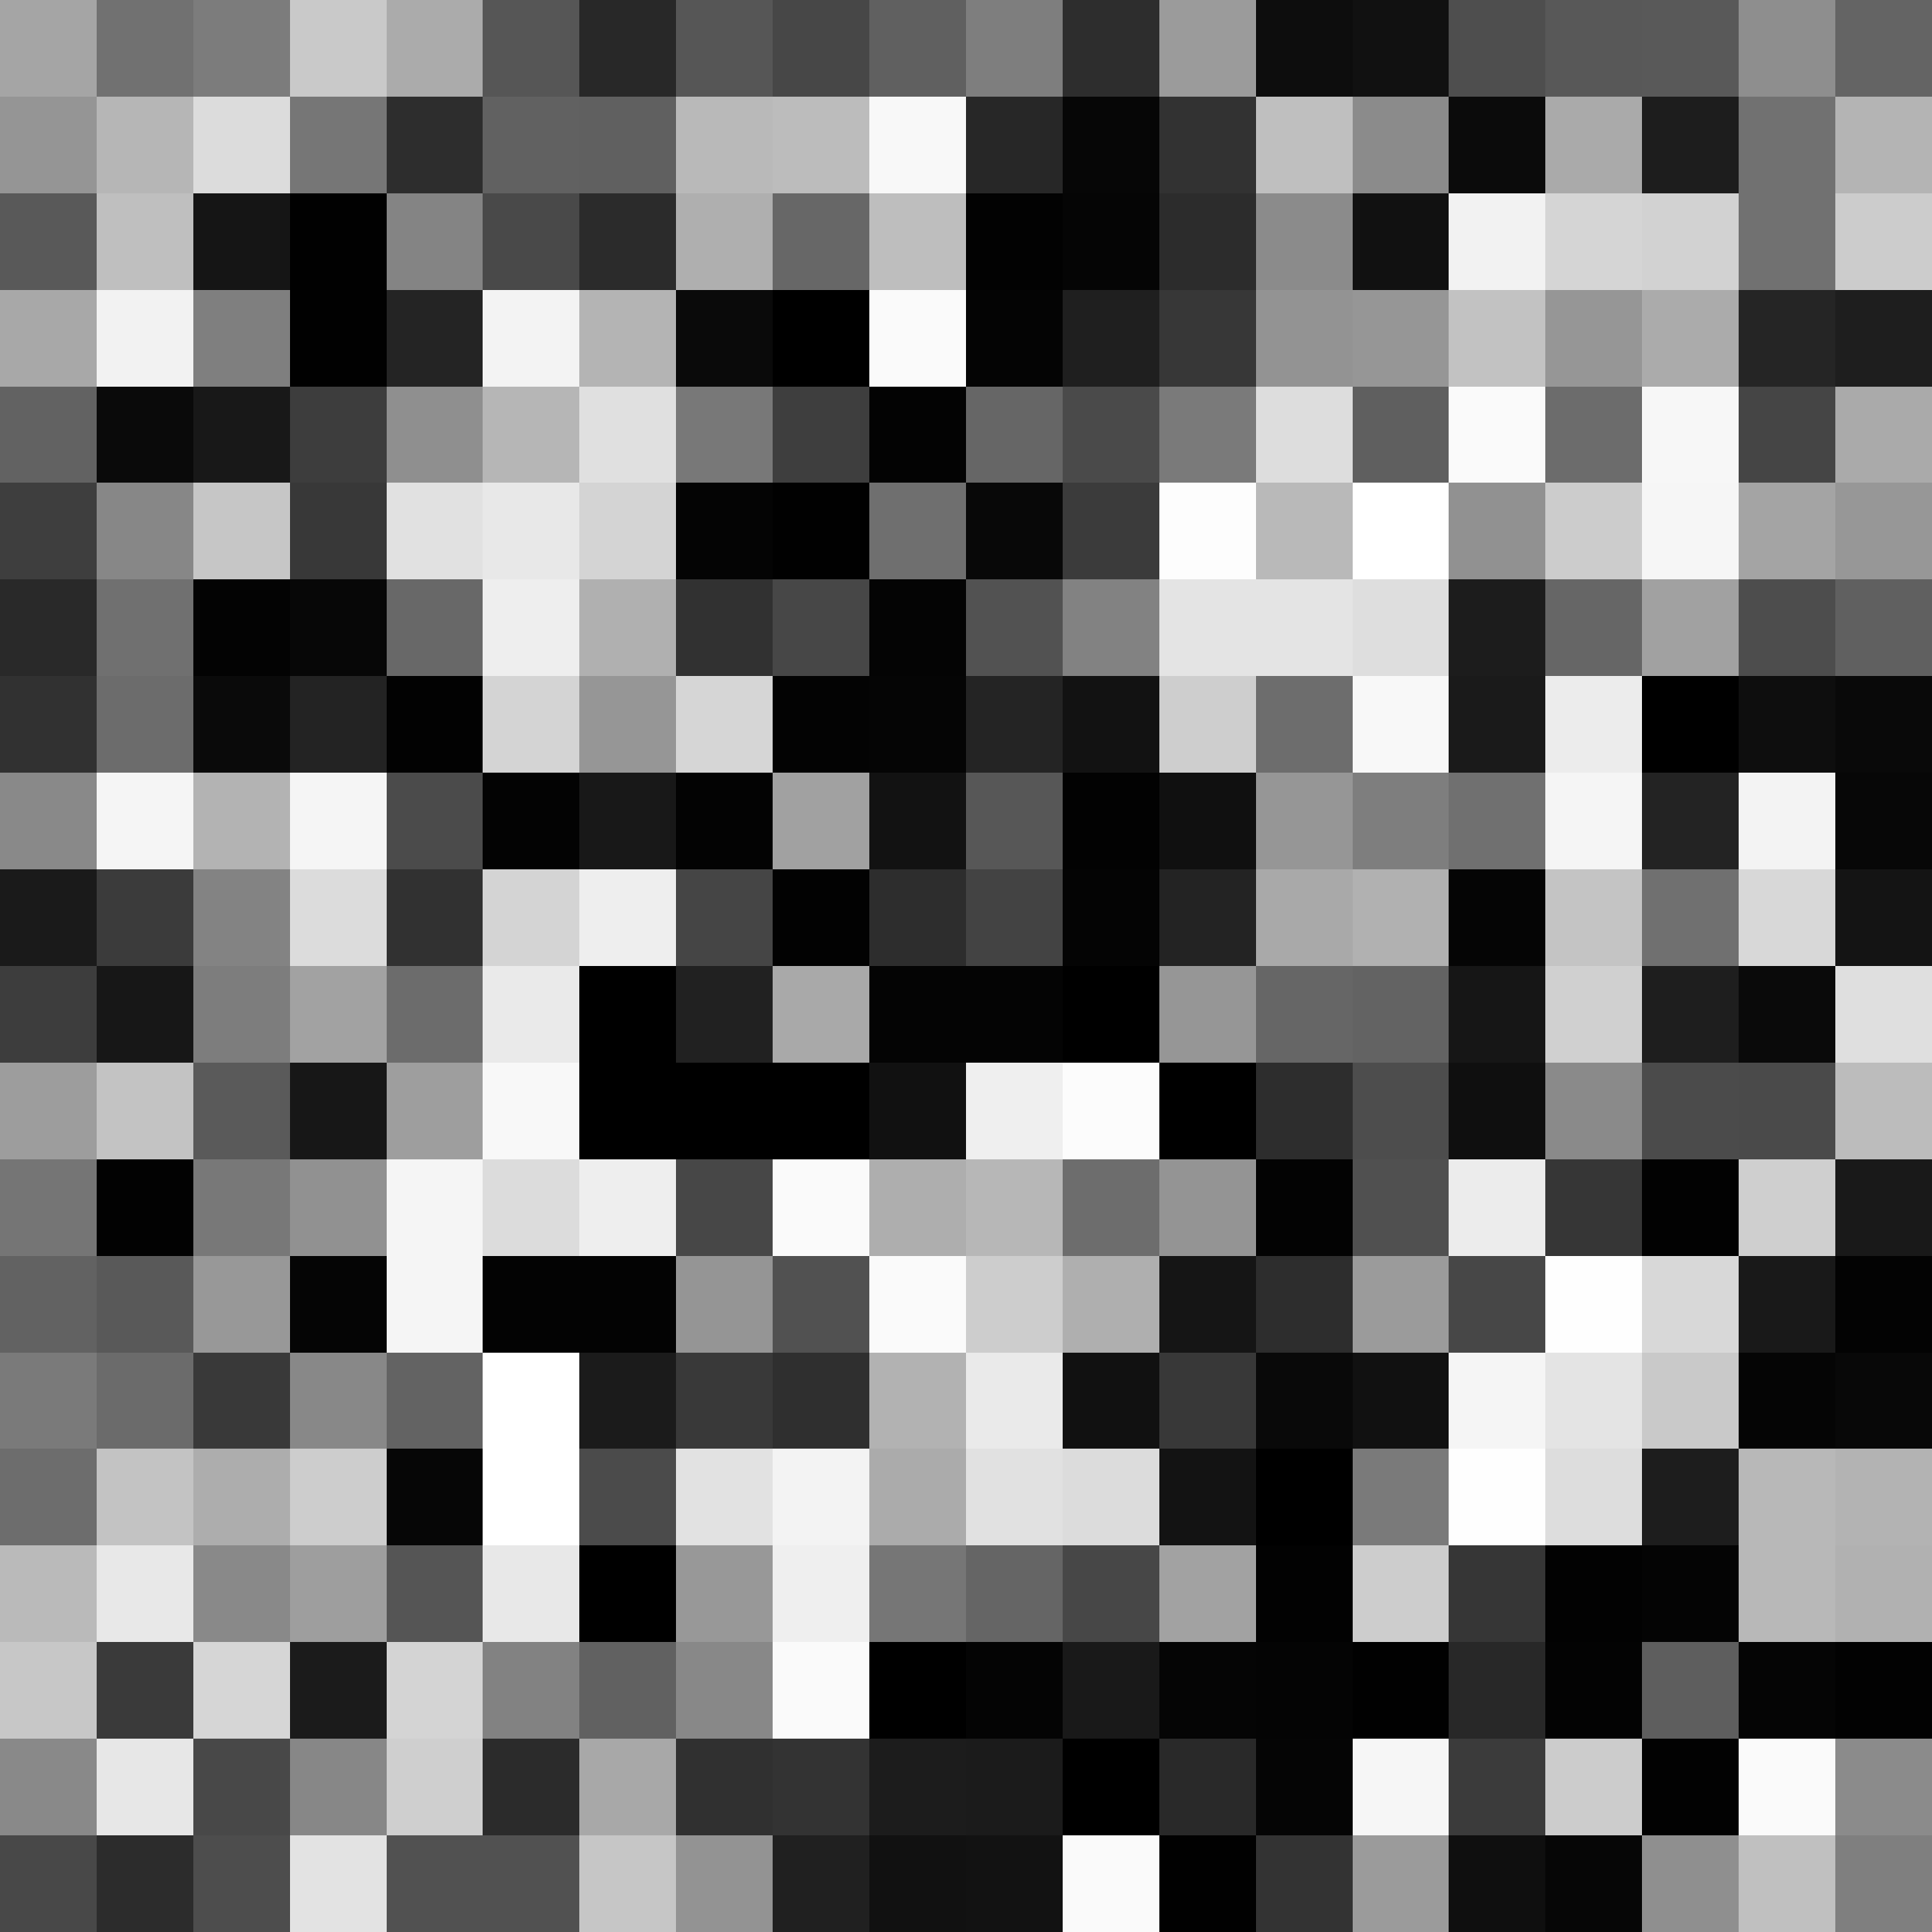
\includegraphics[width=\textwidth]{training_1}
    \end{minipage}
    \begin{minipage}{0.32\textwidth}
        \centering
        
\includegraphics[width=\textwidth]{training_2}
    \end{minipage}
    \begin{minipage}{0.32\textwidth}
        \centering
        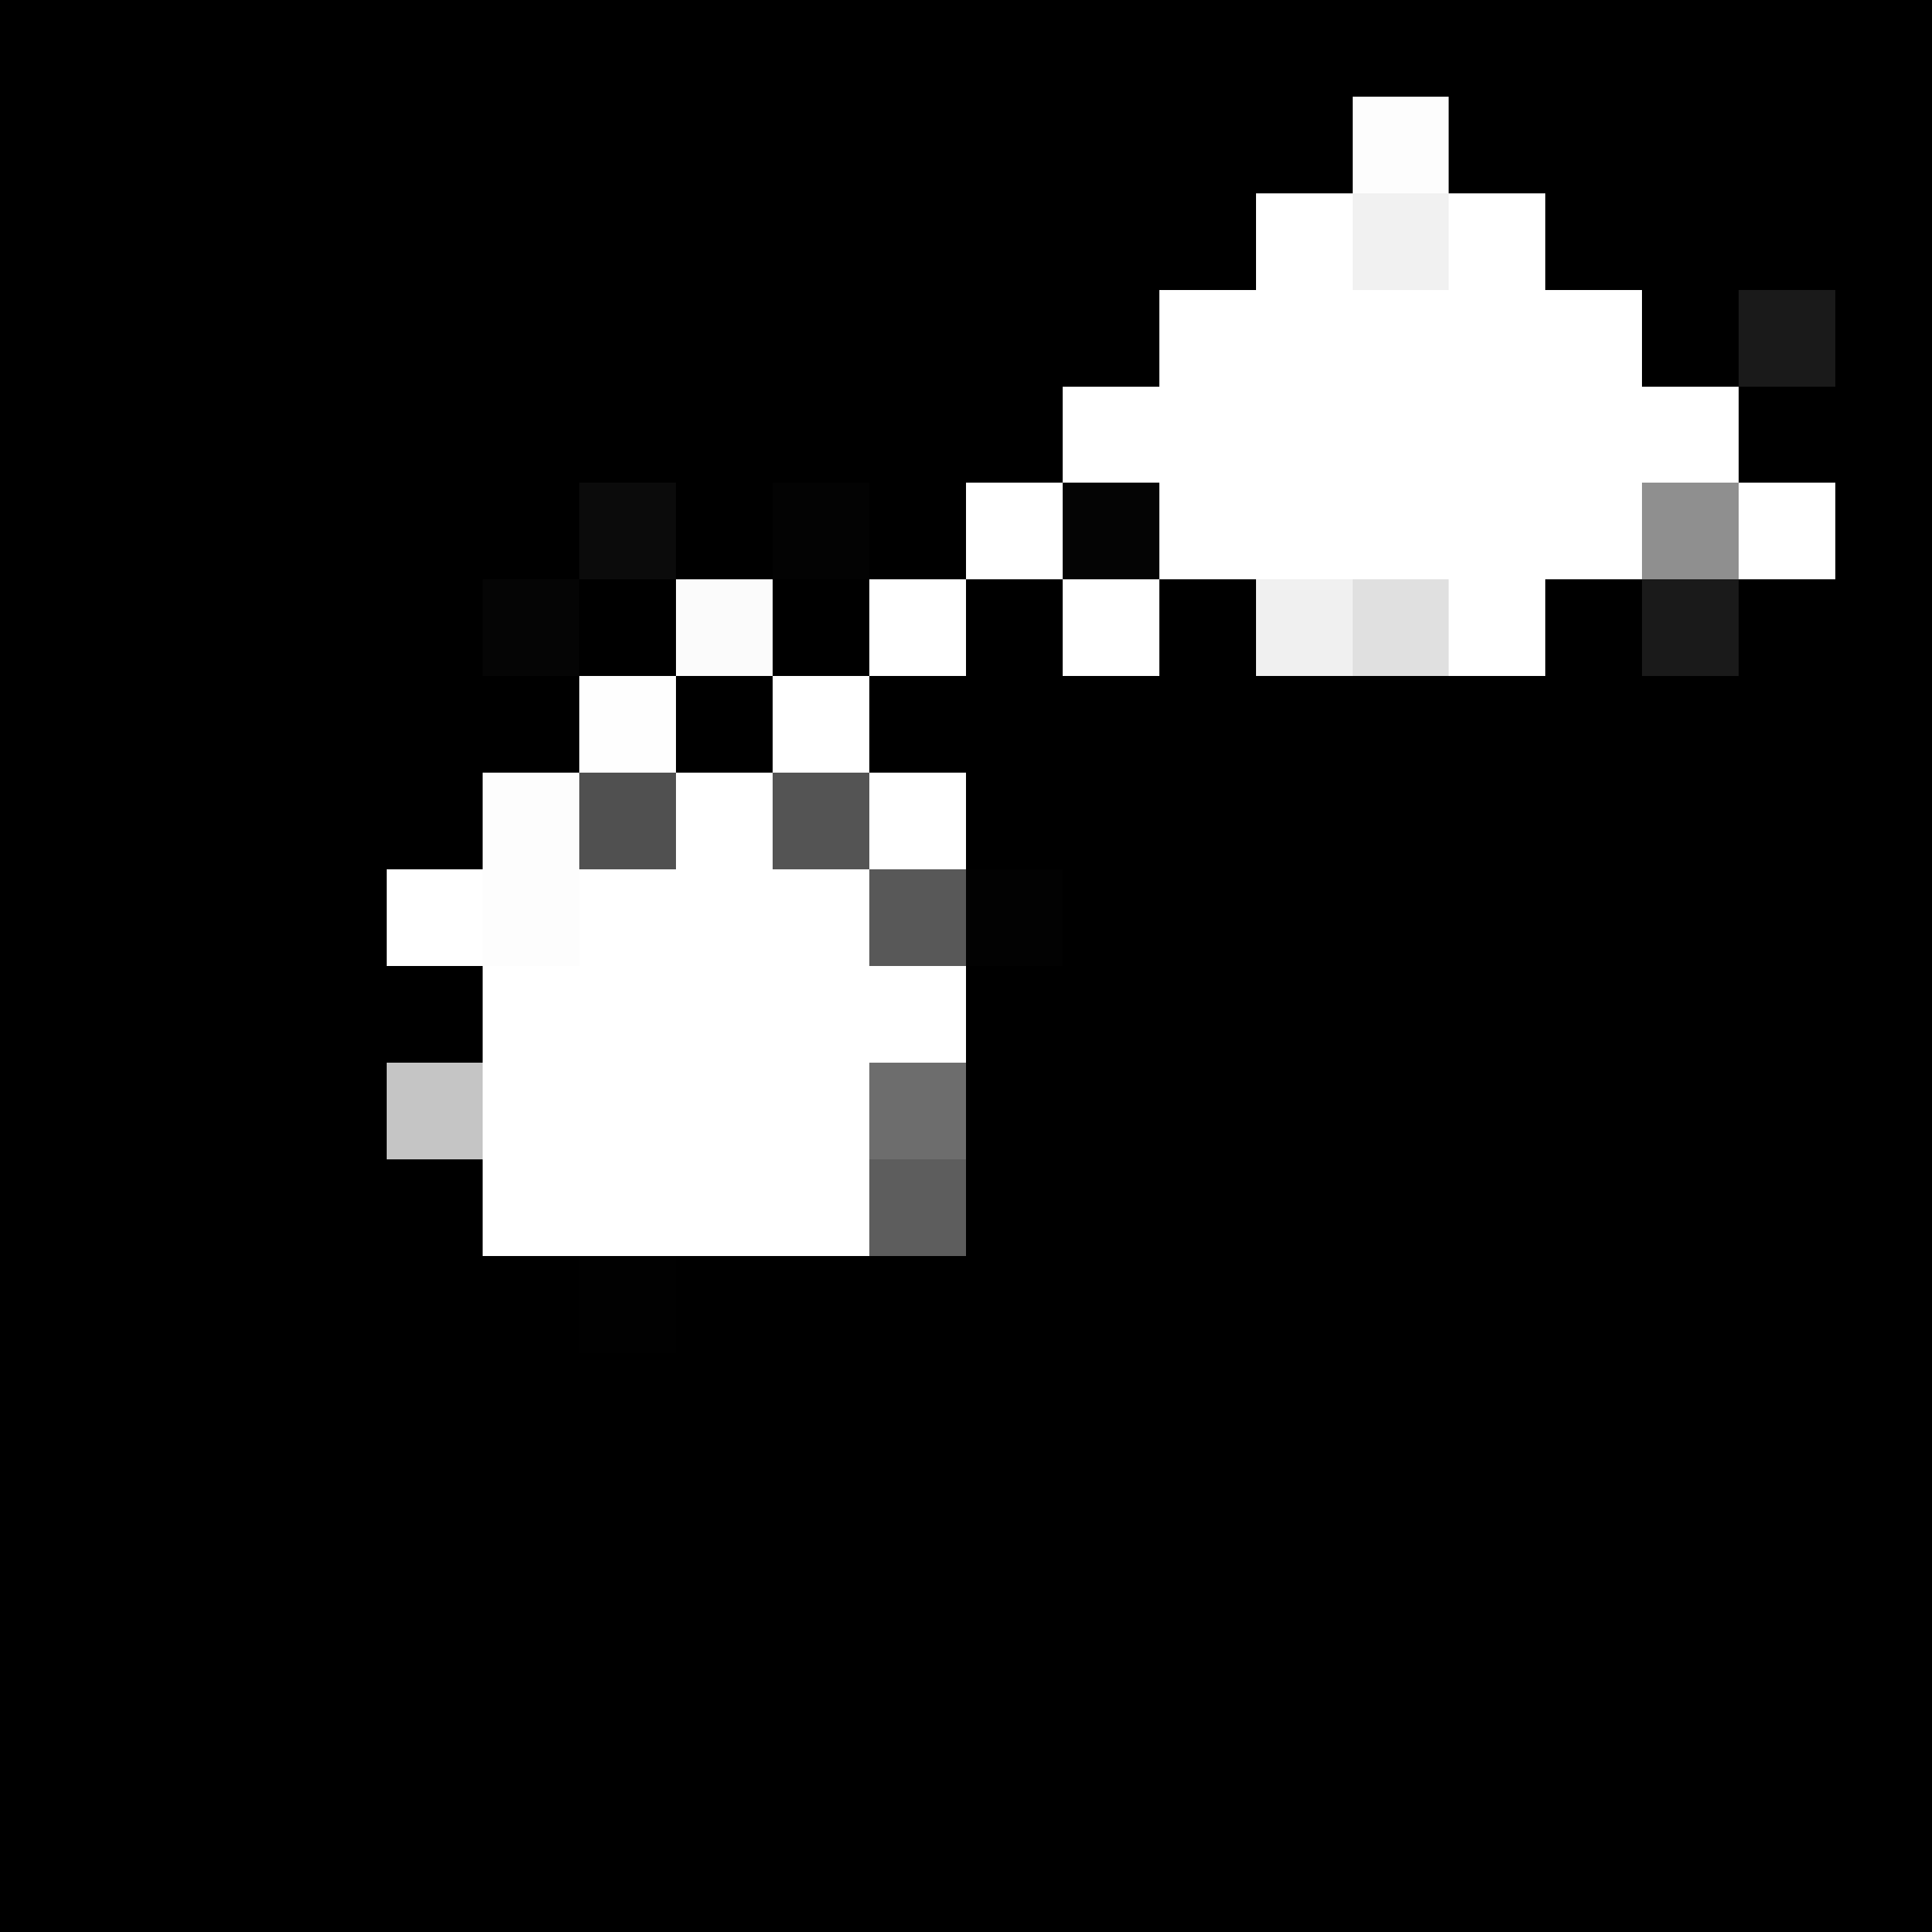
\includegraphics[width=\textwidth]{training_3}
    \end{minipage}
    \vspace{0.3cm}
    \begin{minipage}{0.32\textwidth}
        \centering
        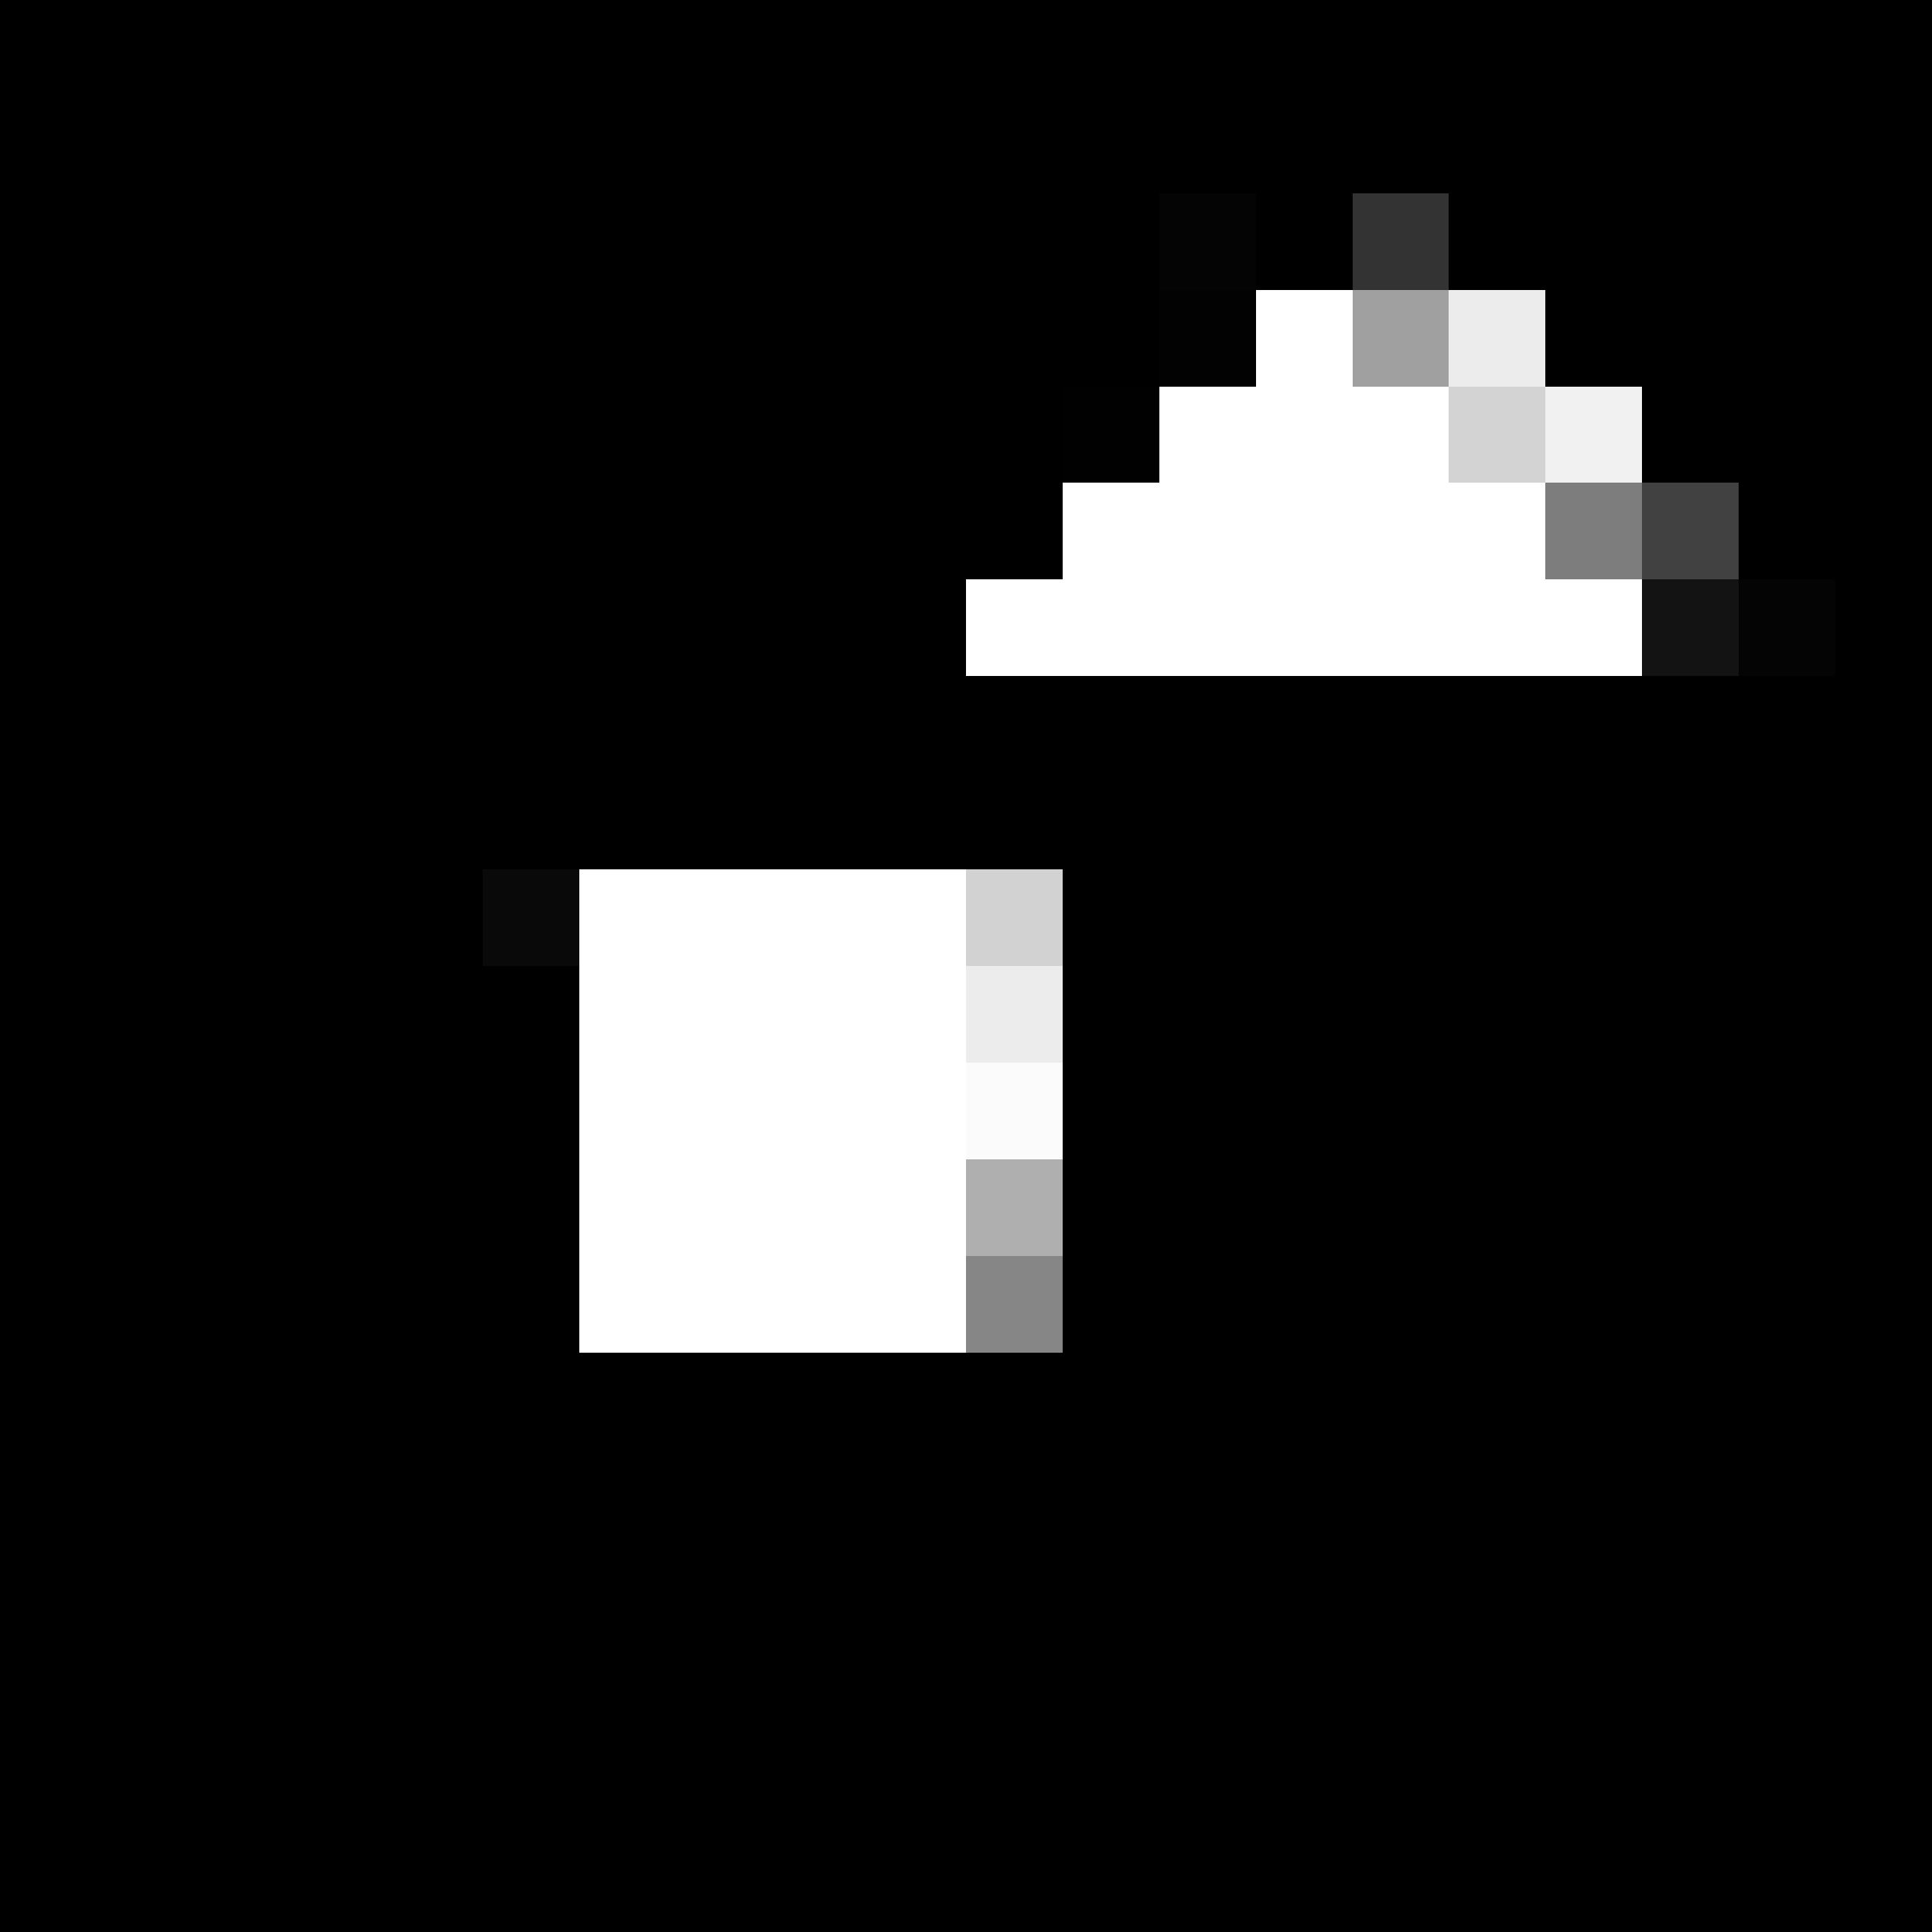
\includegraphics[width=\textwidth]{training_4}
    \end{minipage}
    \begin{minipage}{0.32\textwidth}
        \centering
        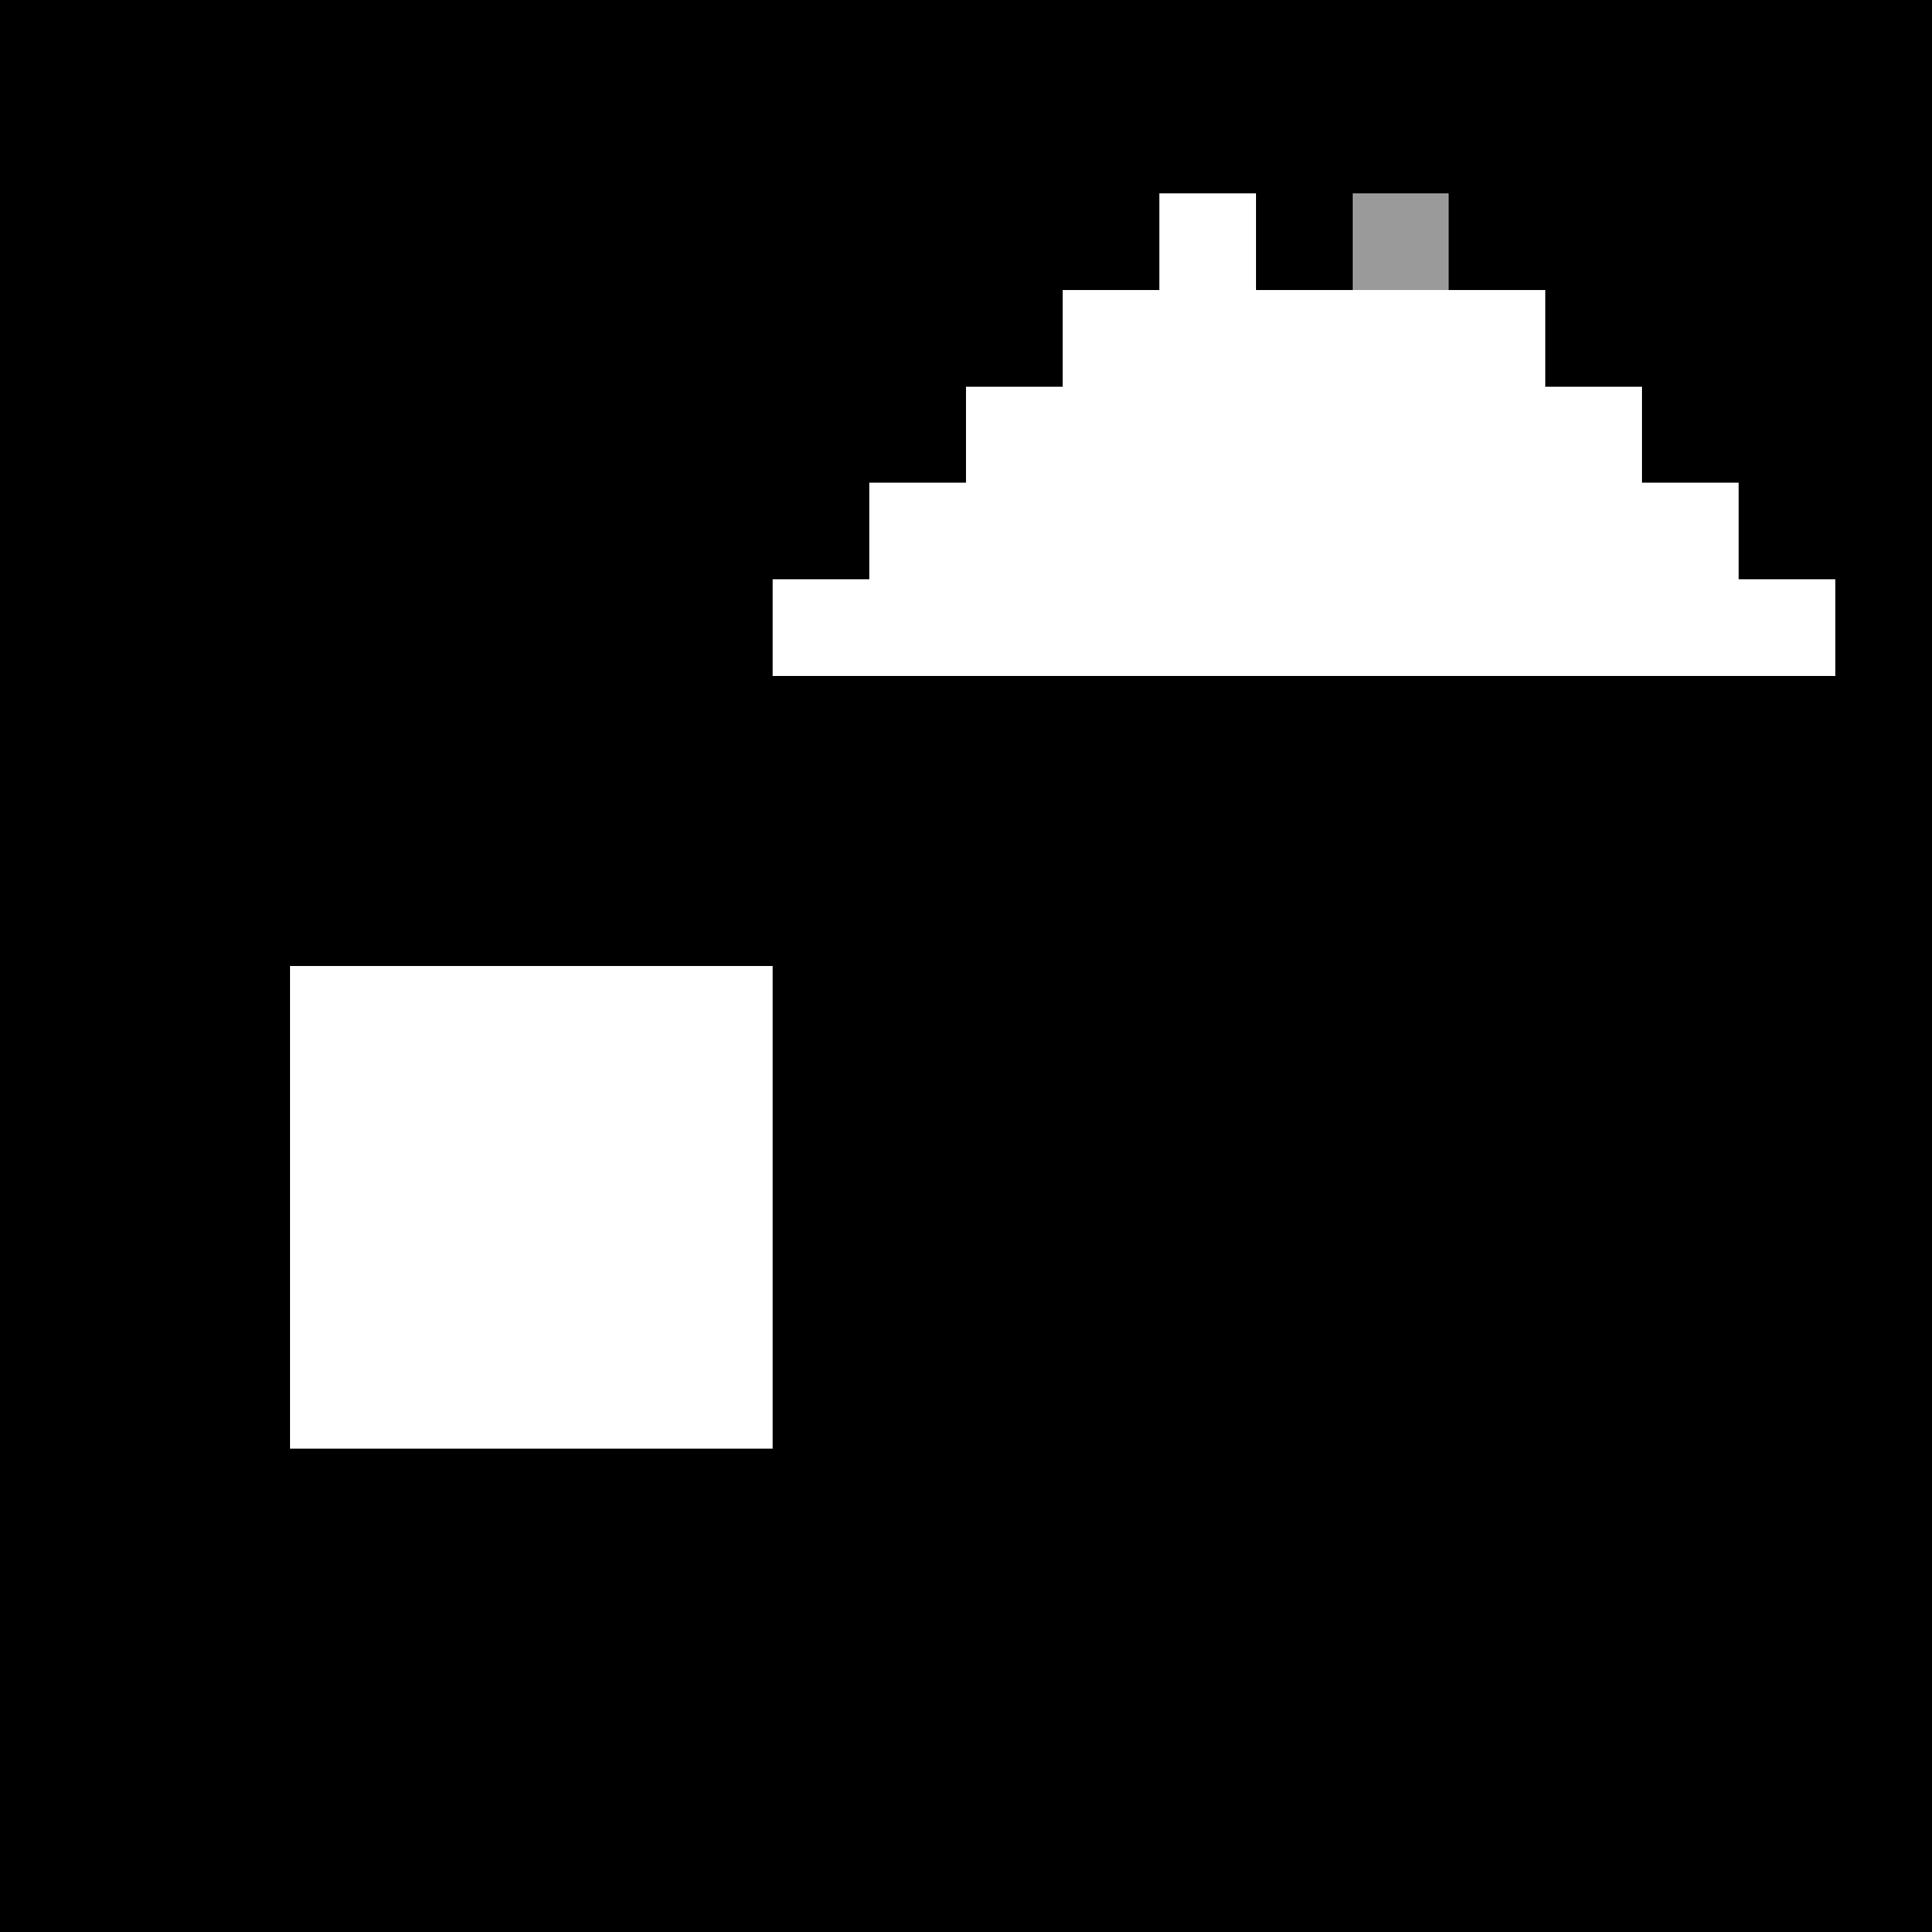
\includegraphics[width=\textwidth]{training_5}
    \end{minipage}
    \begin{minipage}{0.32\textwidth}
        \centering
        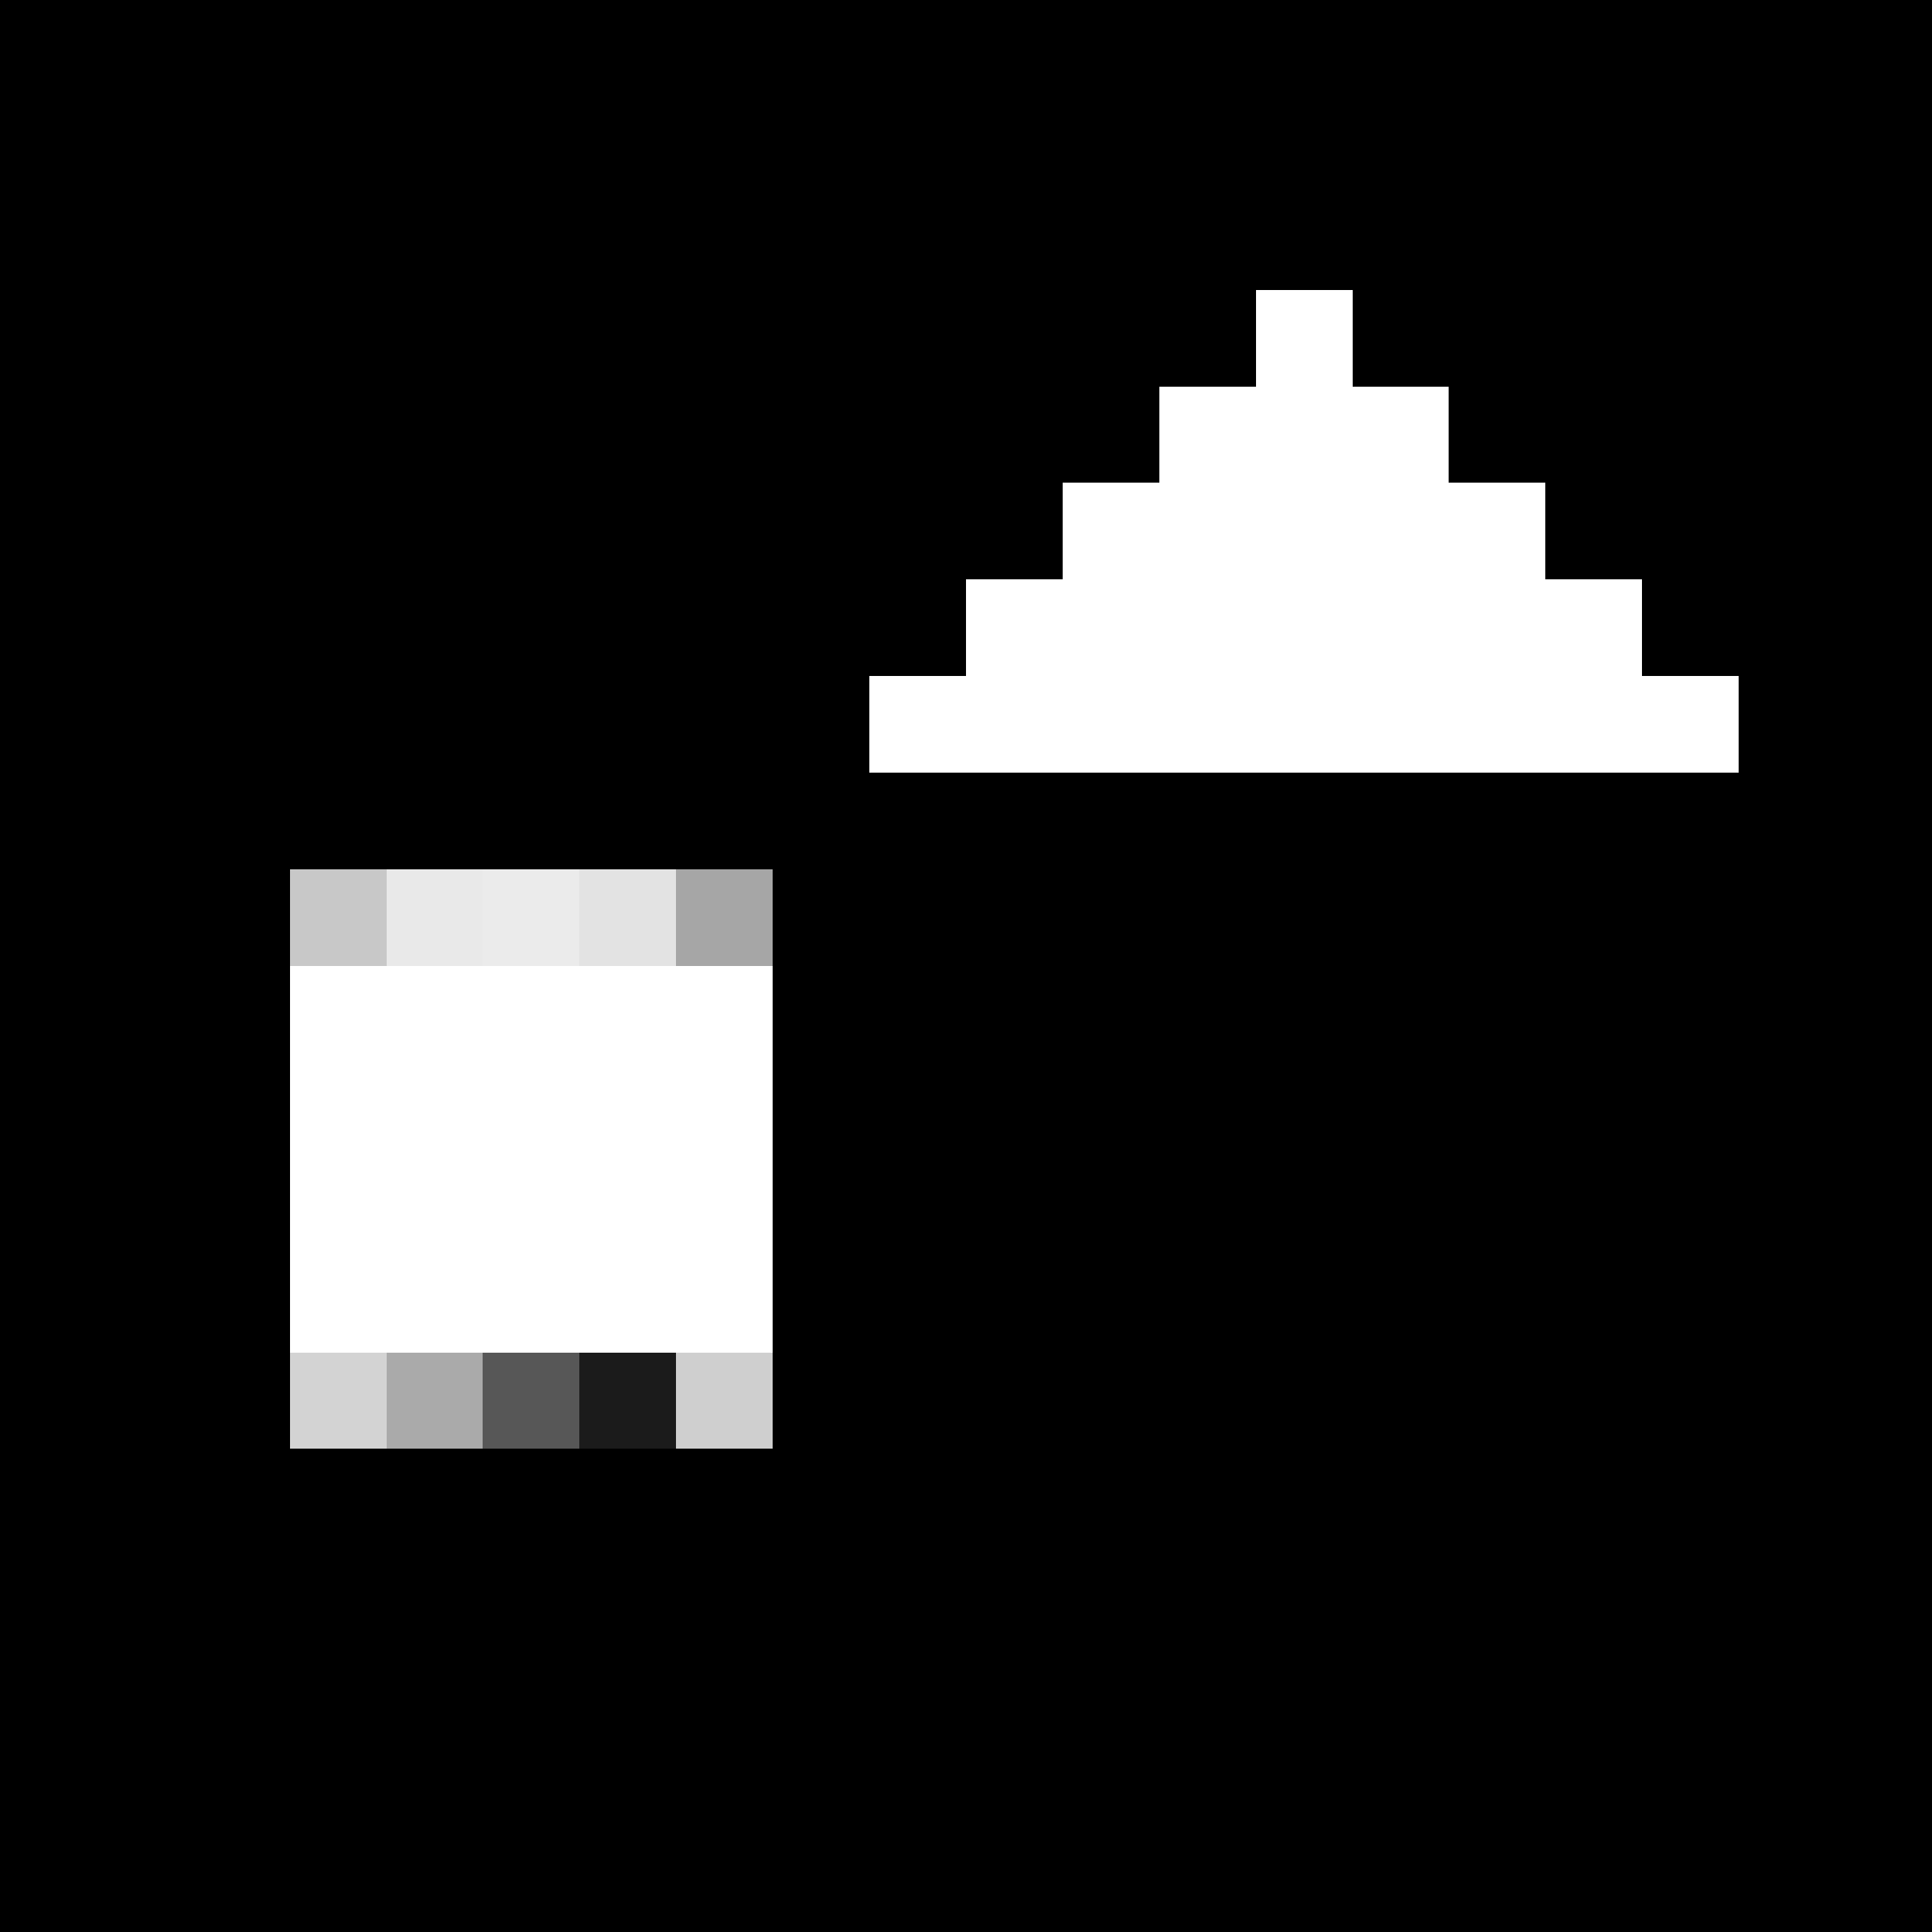
\includegraphics[width=\textwidth]{training_6}
    \end{minipage}
    \caption{Samples drawn at different epochs from the generator trained on \textit{poly20} (zoom).}
\end{figure}


\begin{figure}[ht]
    \centering
    \begin{minipage}{0.32\textwidth}
        \centering
        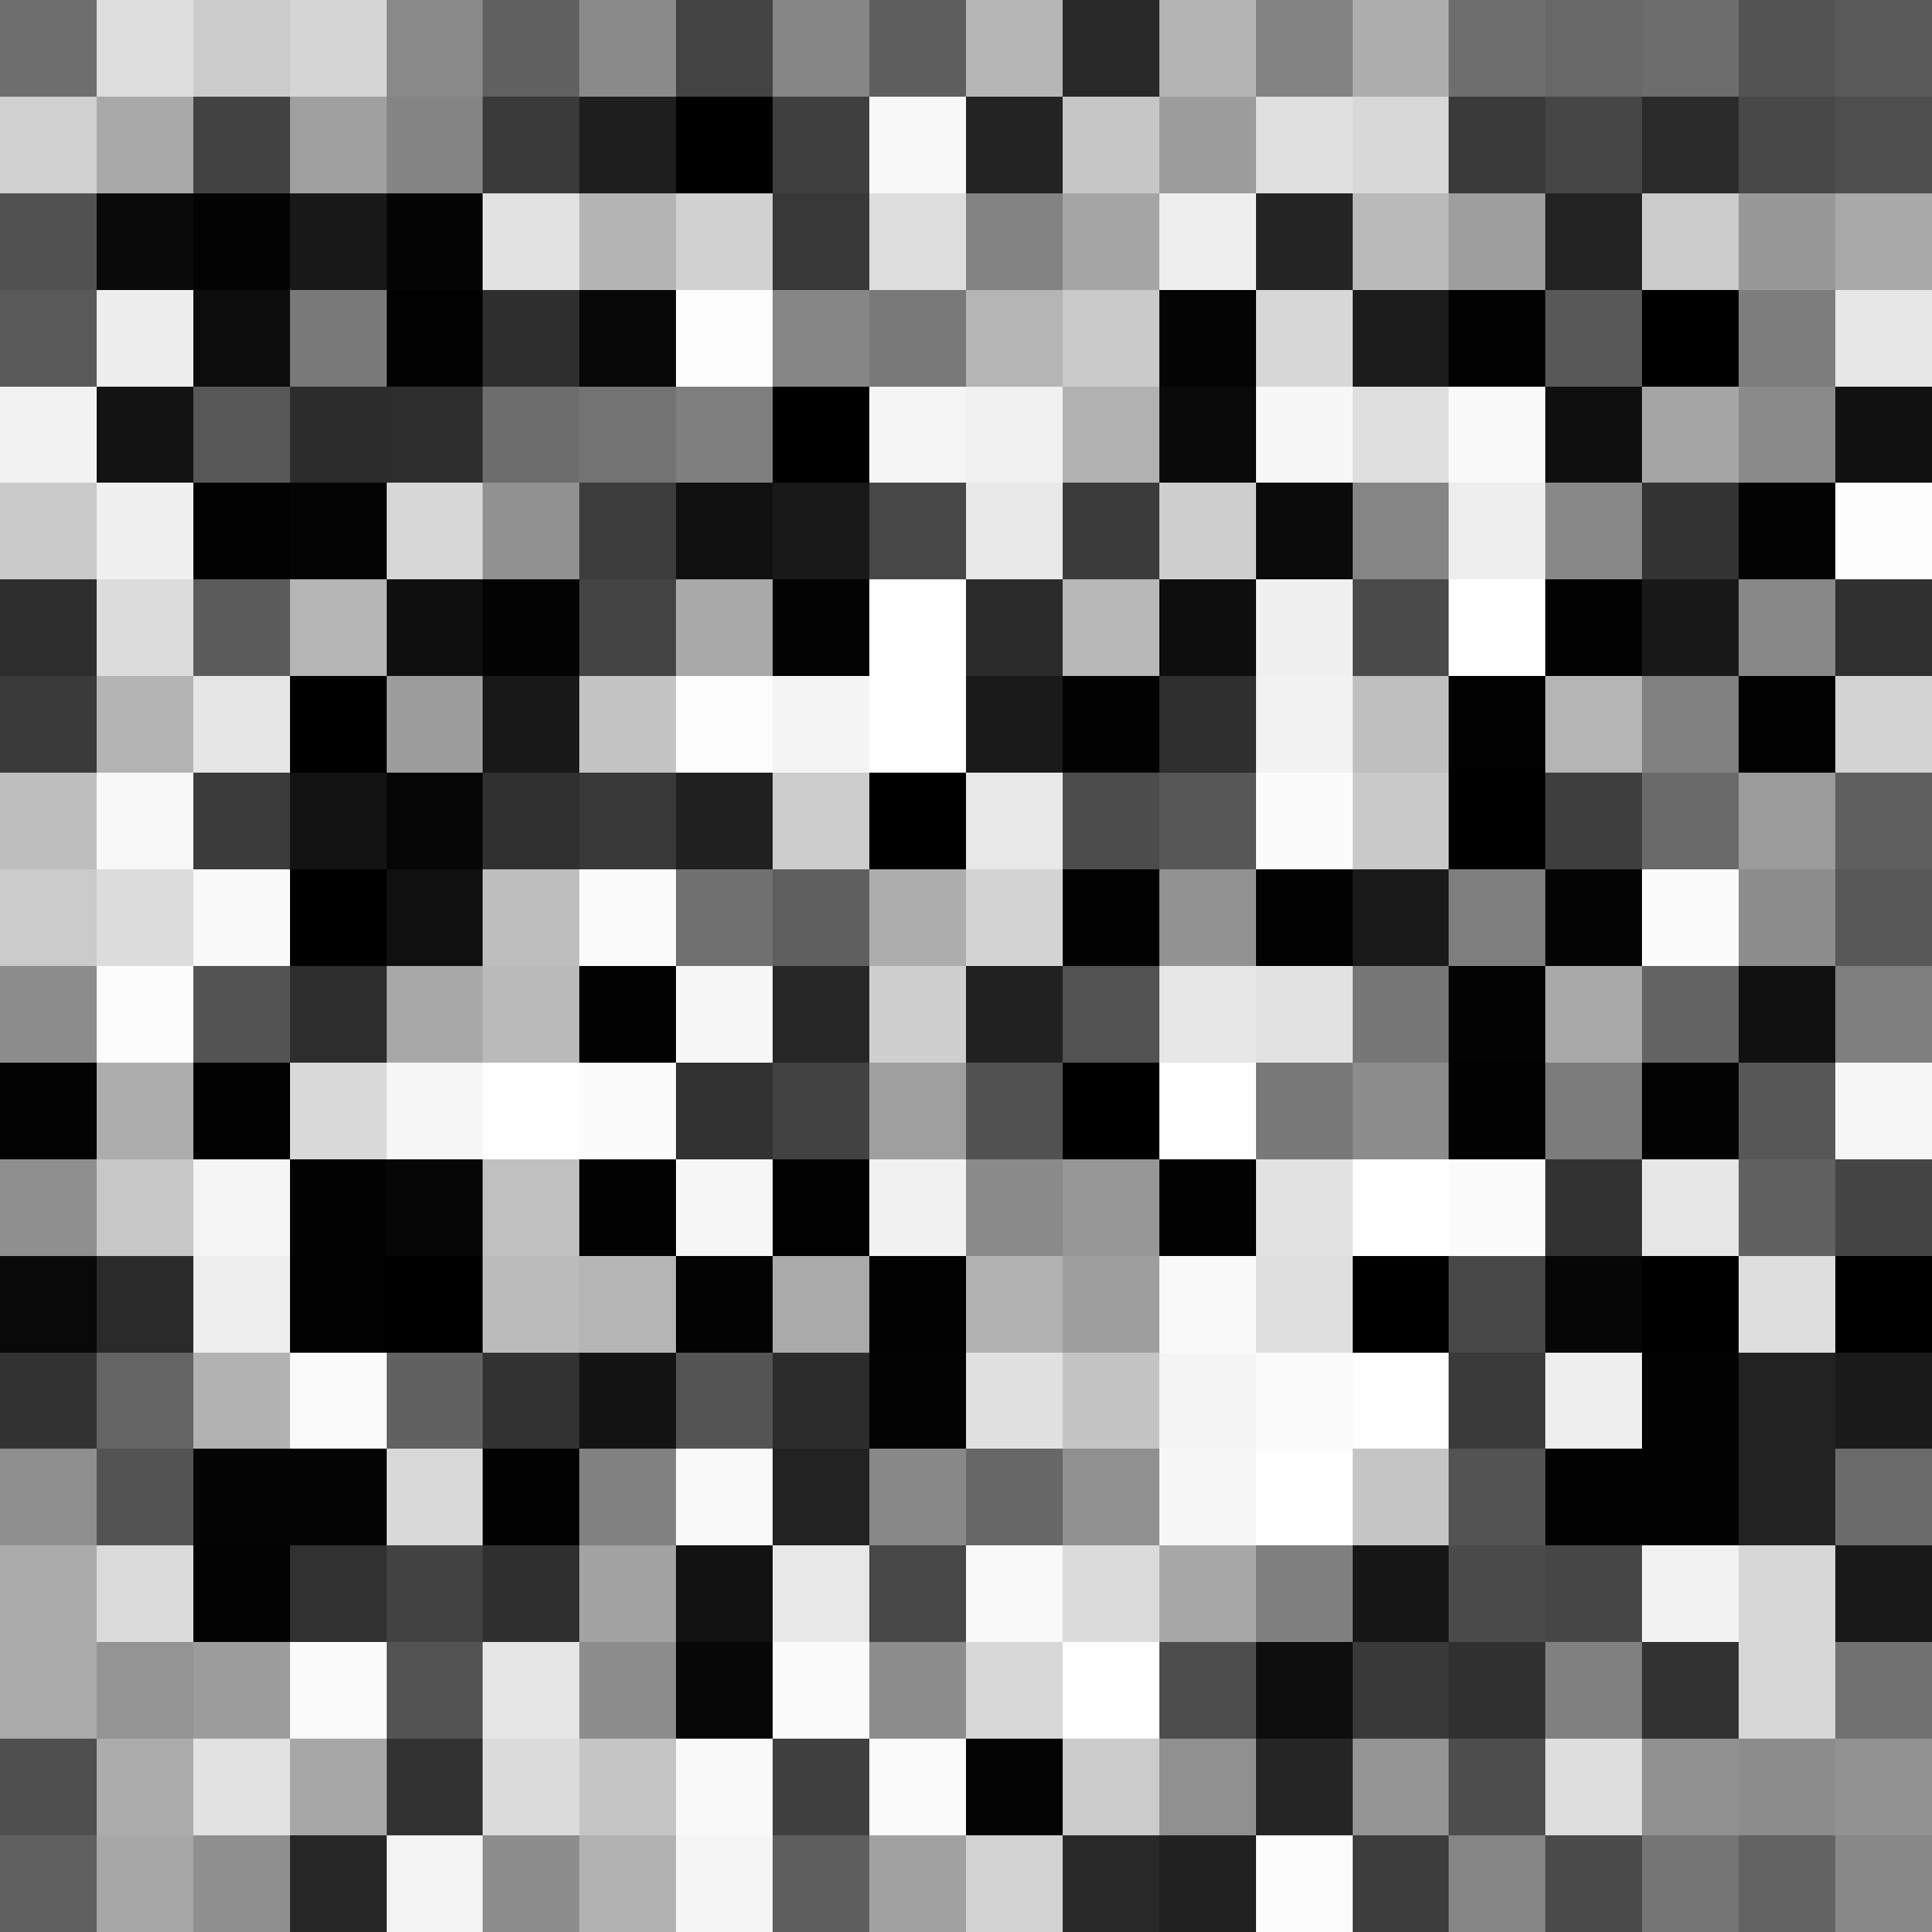
\includegraphics[width=\textwidth]{training_pc_1}
    \end{minipage}
    \begin{minipage}{0.32\textwidth}
        \centering
        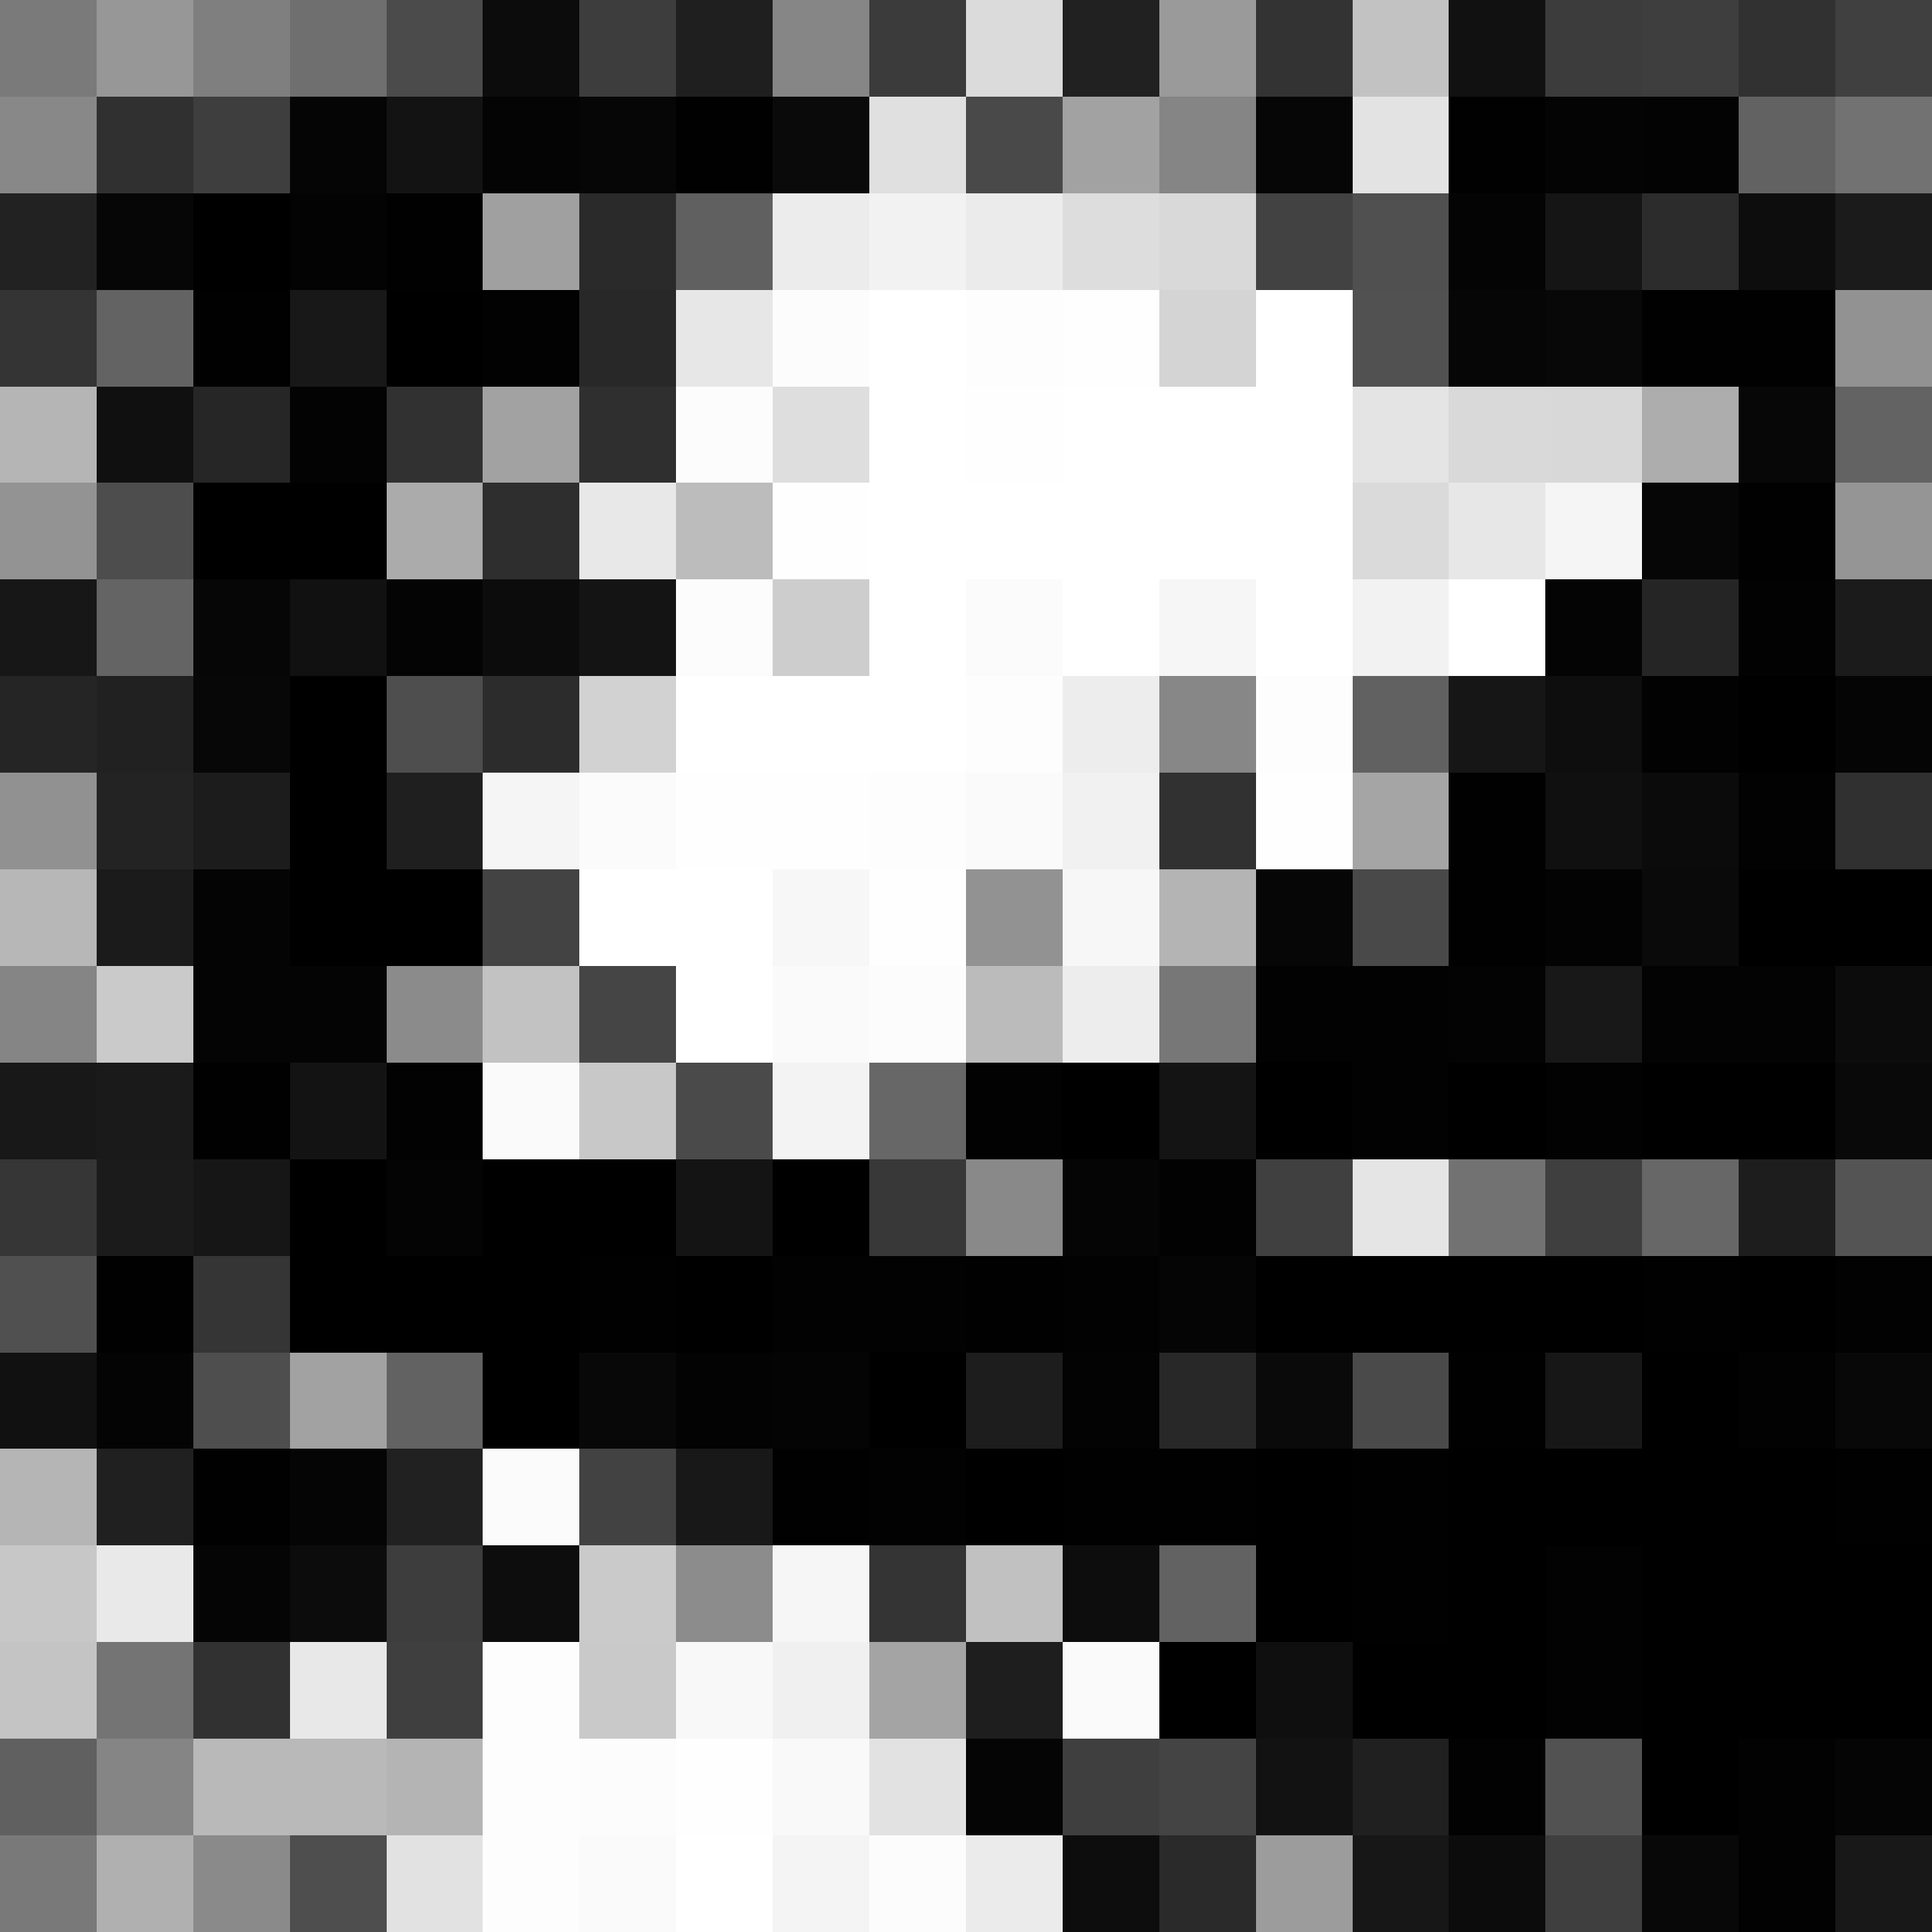
\includegraphics[width=\textwidth]{training_pc_2}
    \end{minipage}
    \begin{minipage}{0.32\textwidth}
        \centering
        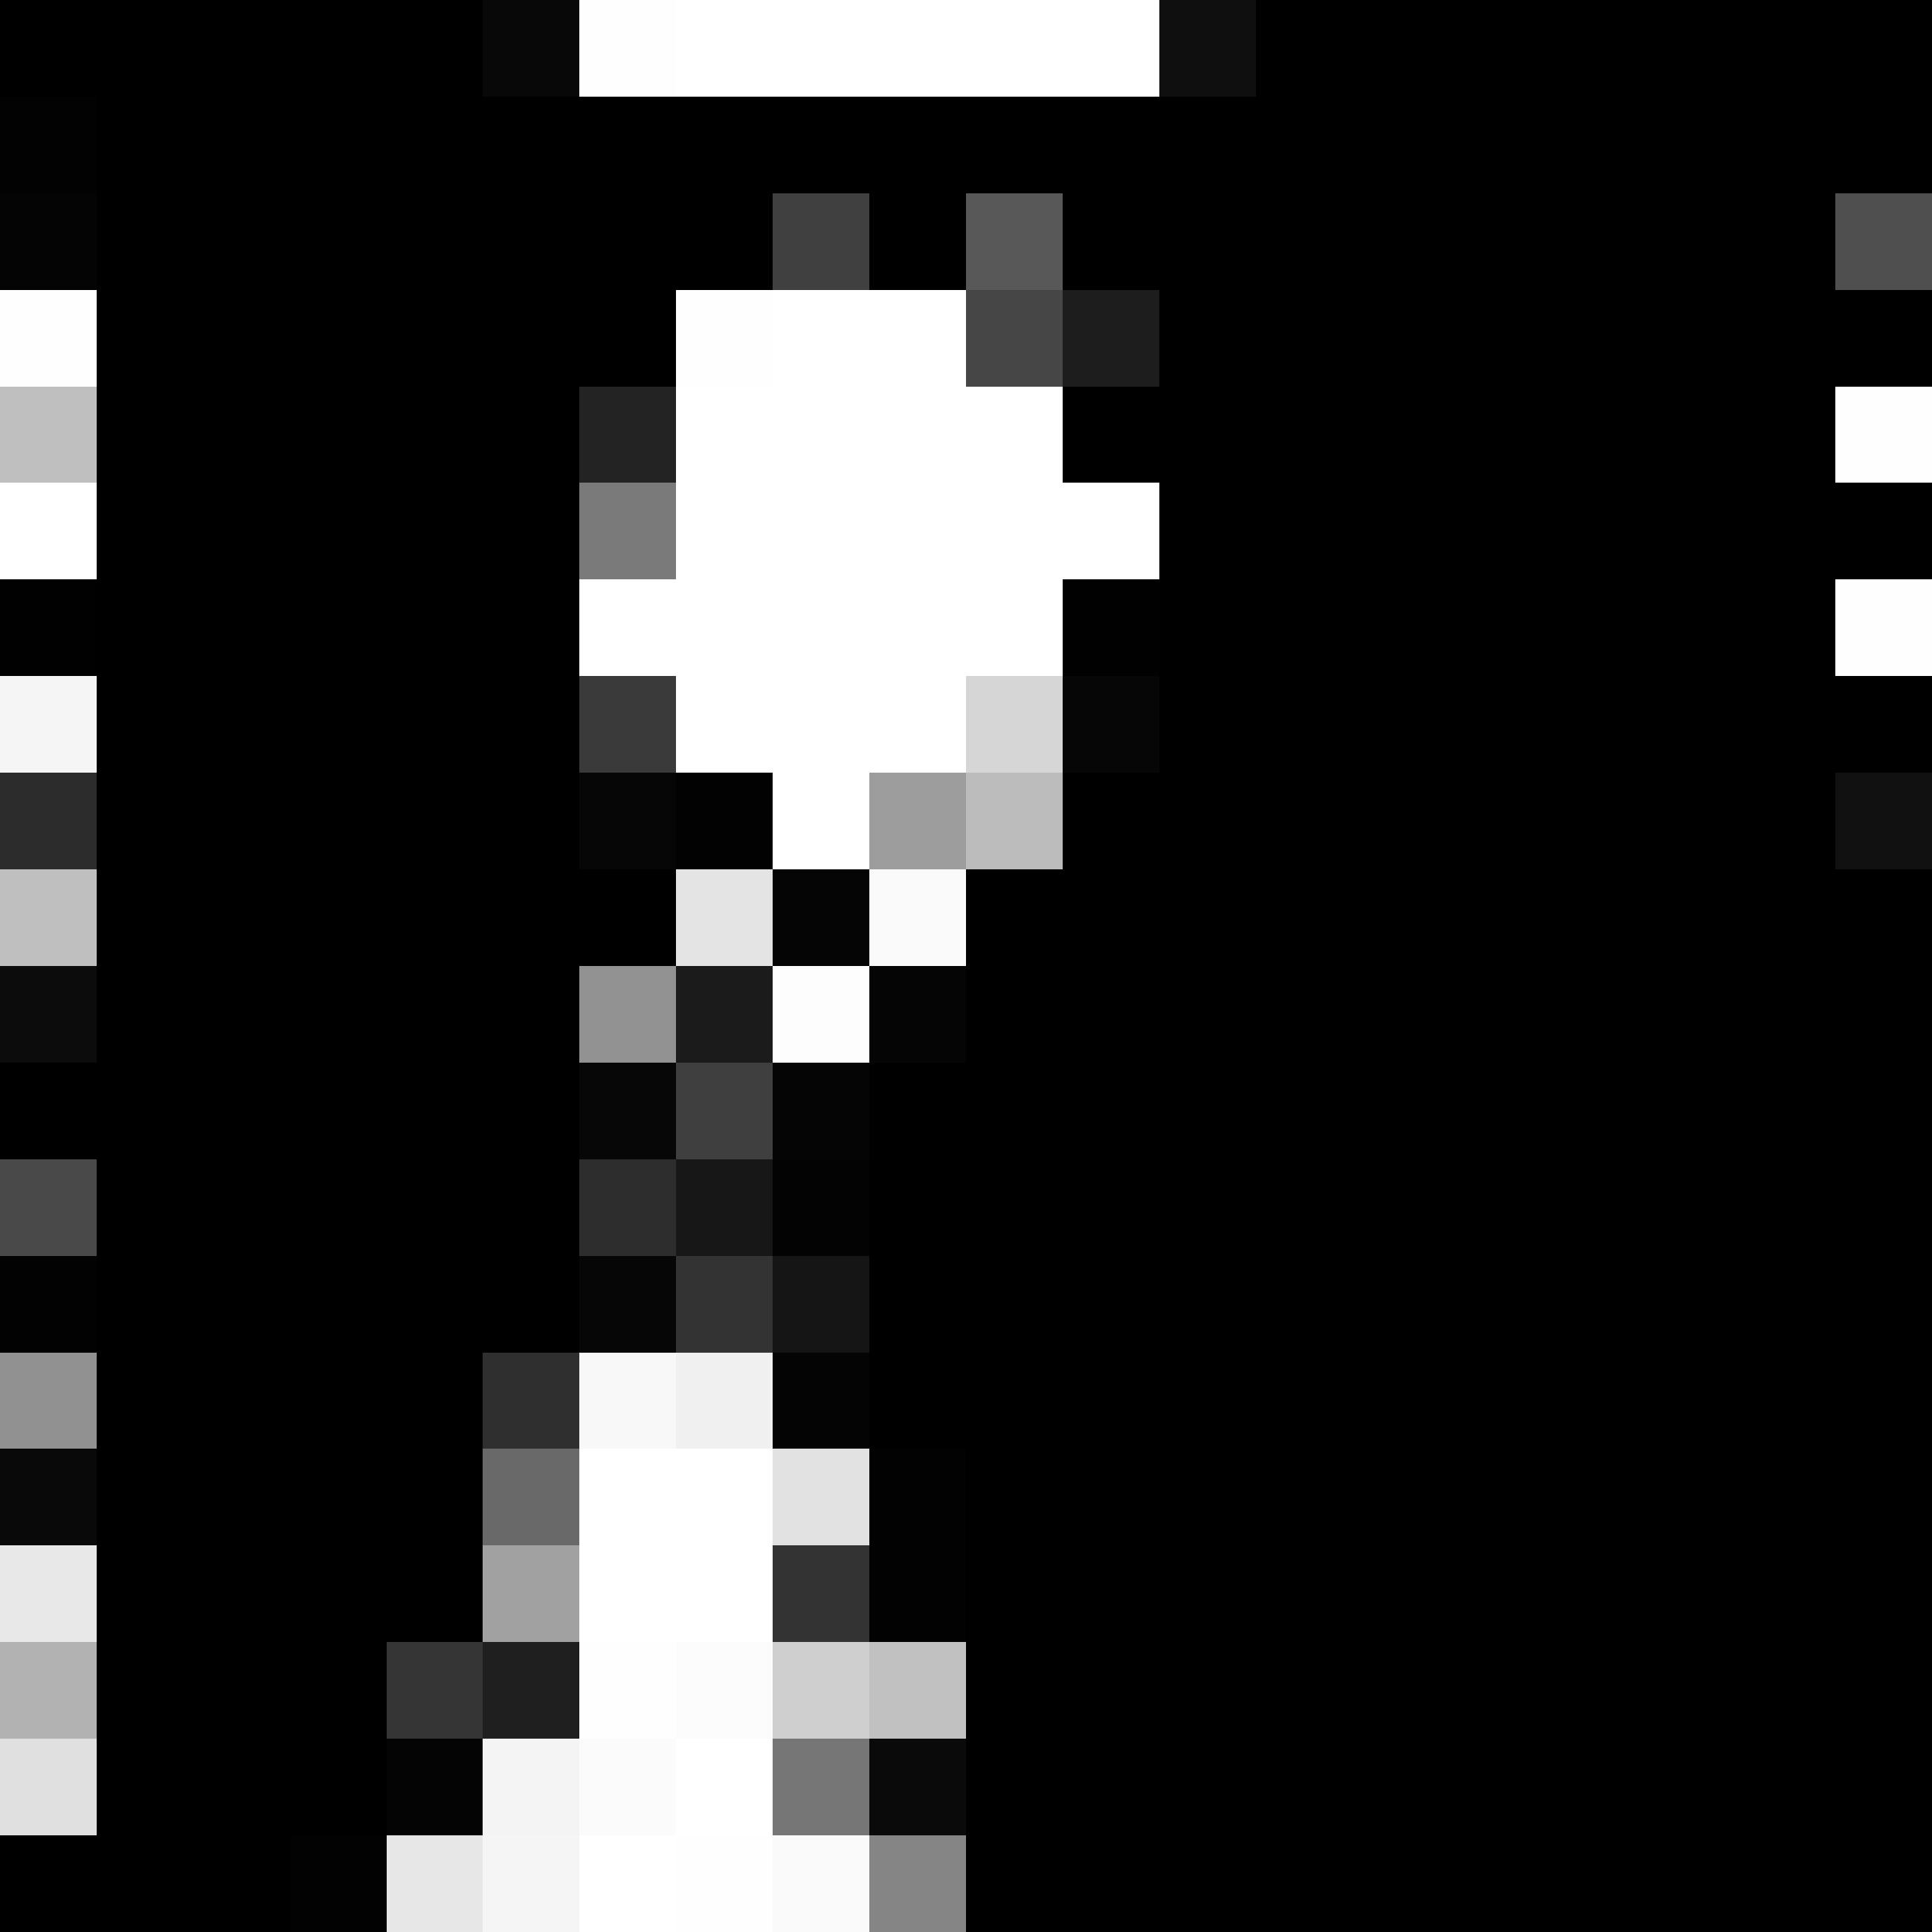
\includegraphics[width=\textwidth]{training_pc_3}
    \end{minipage}
    \vspace{0.3cm}
    \begin{minipage}{0.32\textwidth}
        \centering
        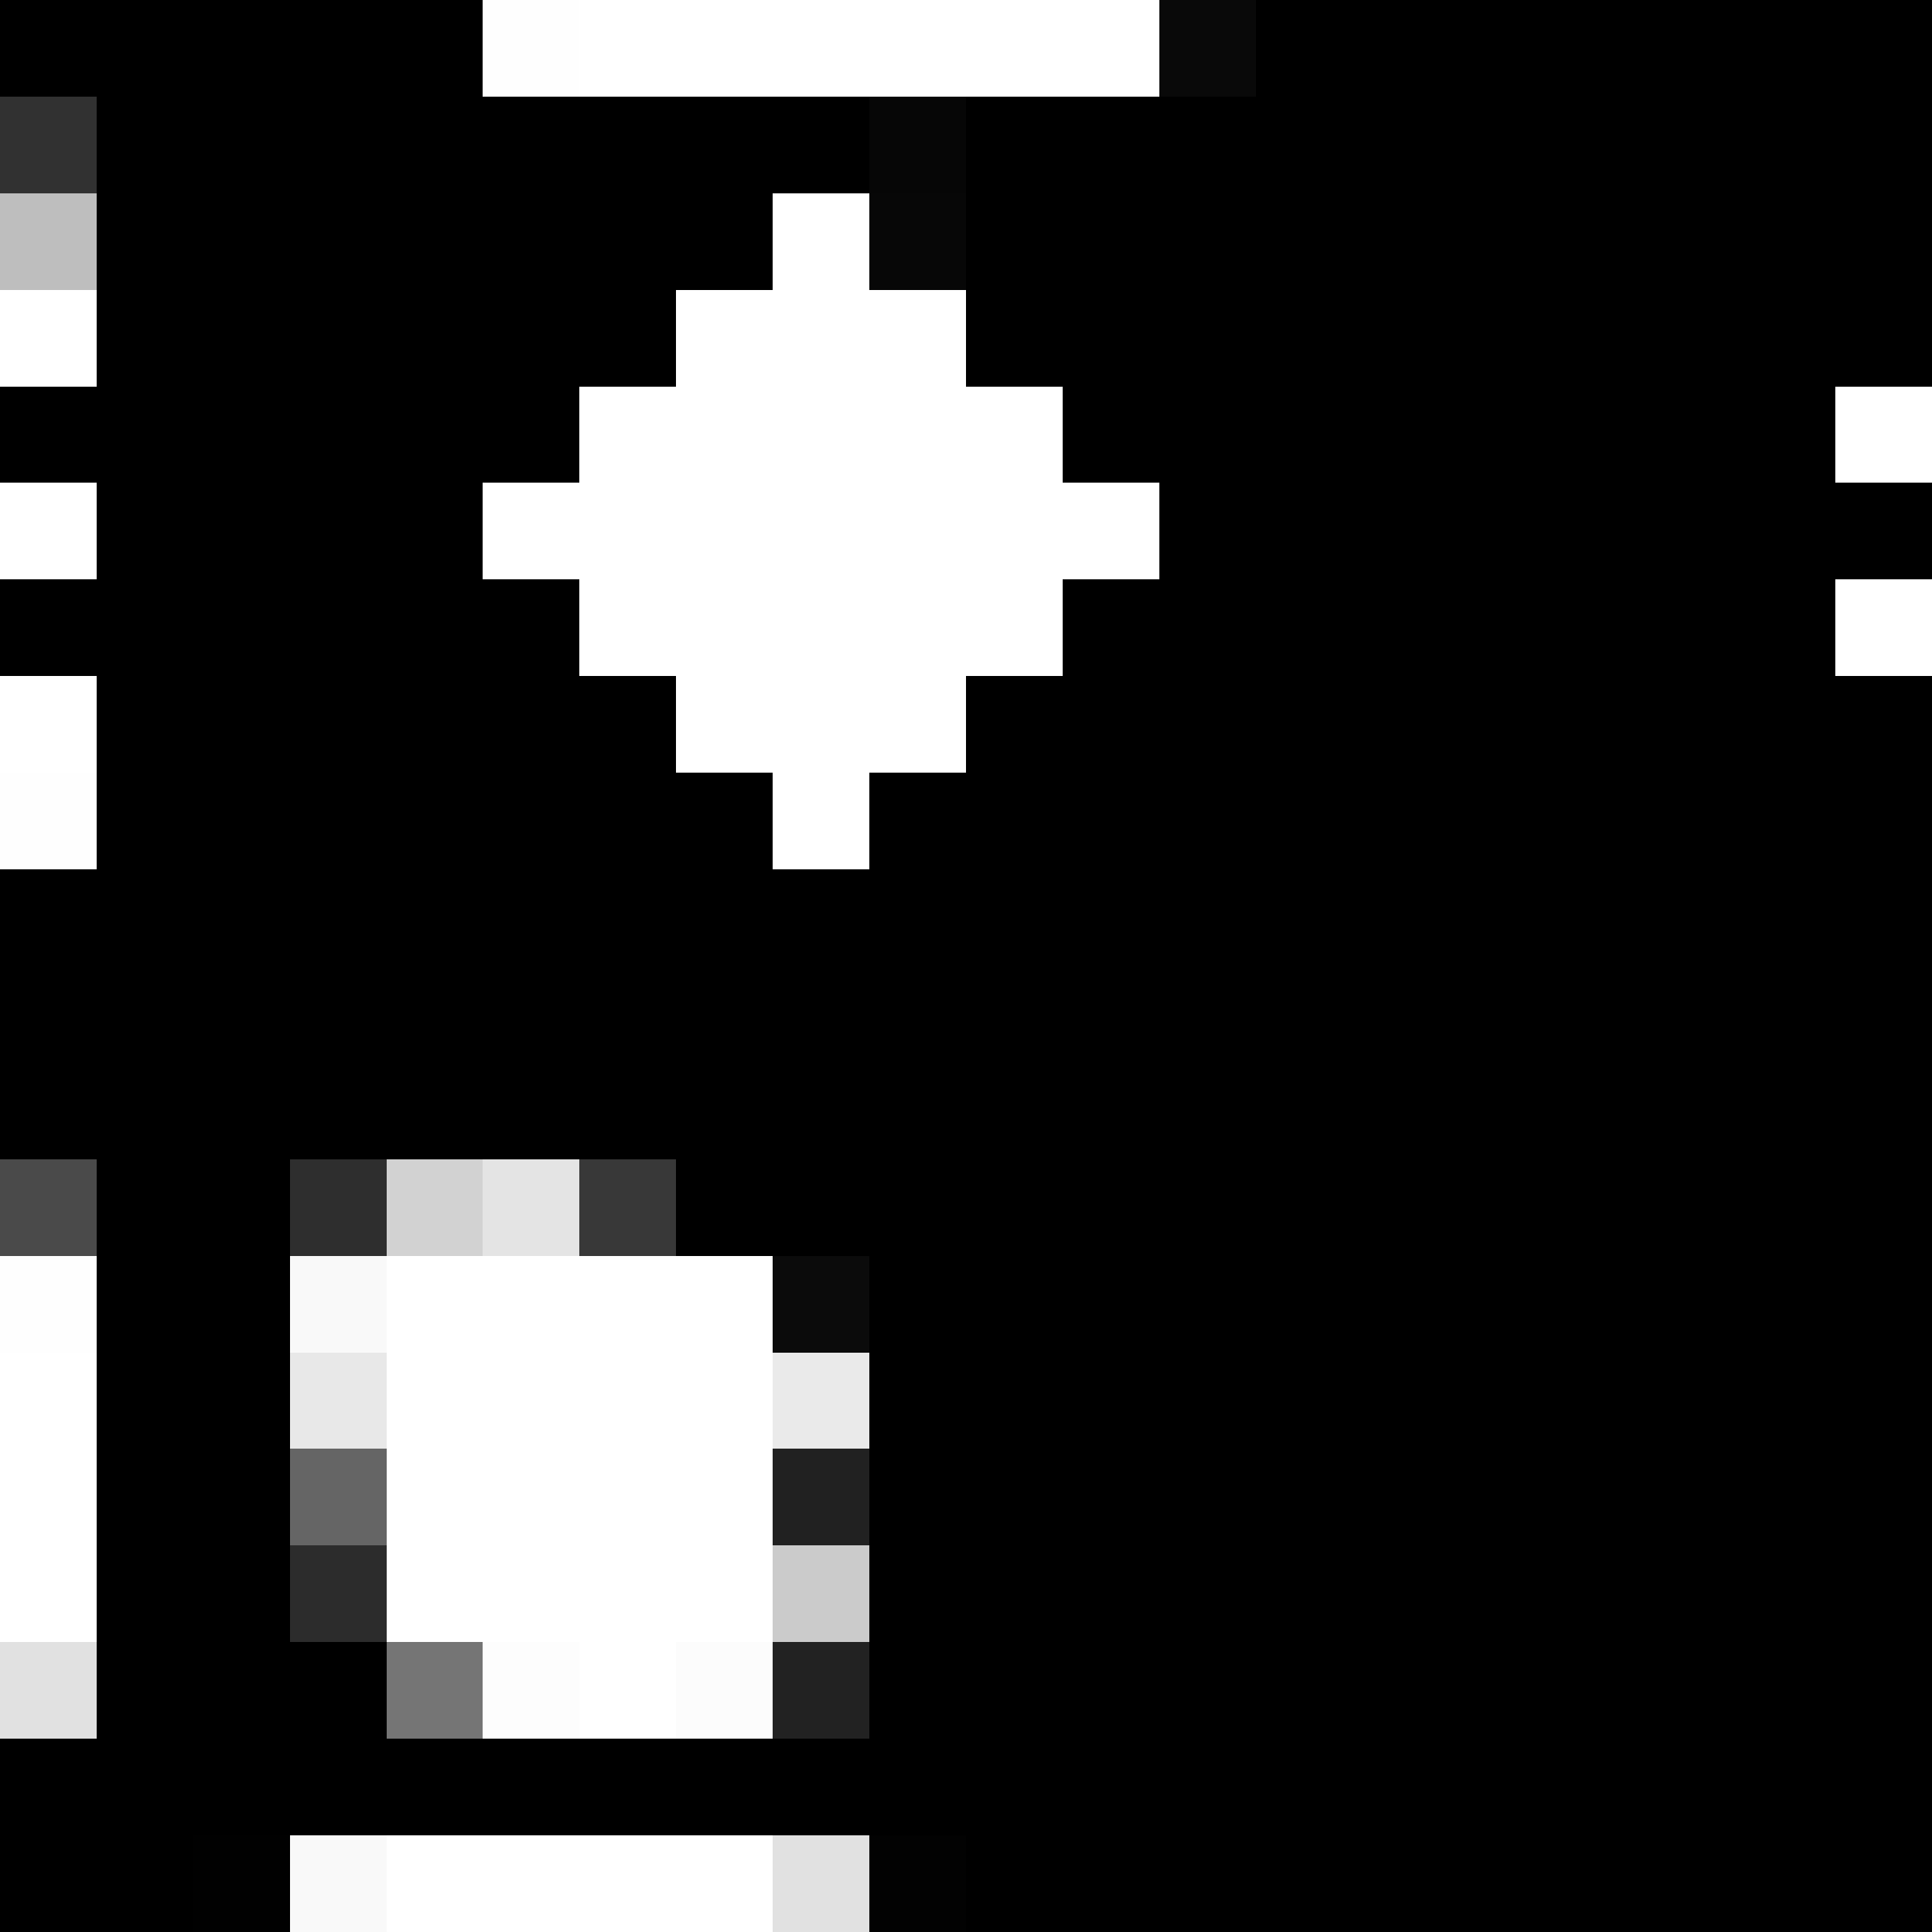
\includegraphics[width=\textwidth]{training_pc_4}
    \end{minipage}
    \begin{minipage}{0.32\textwidth}
        \centering
        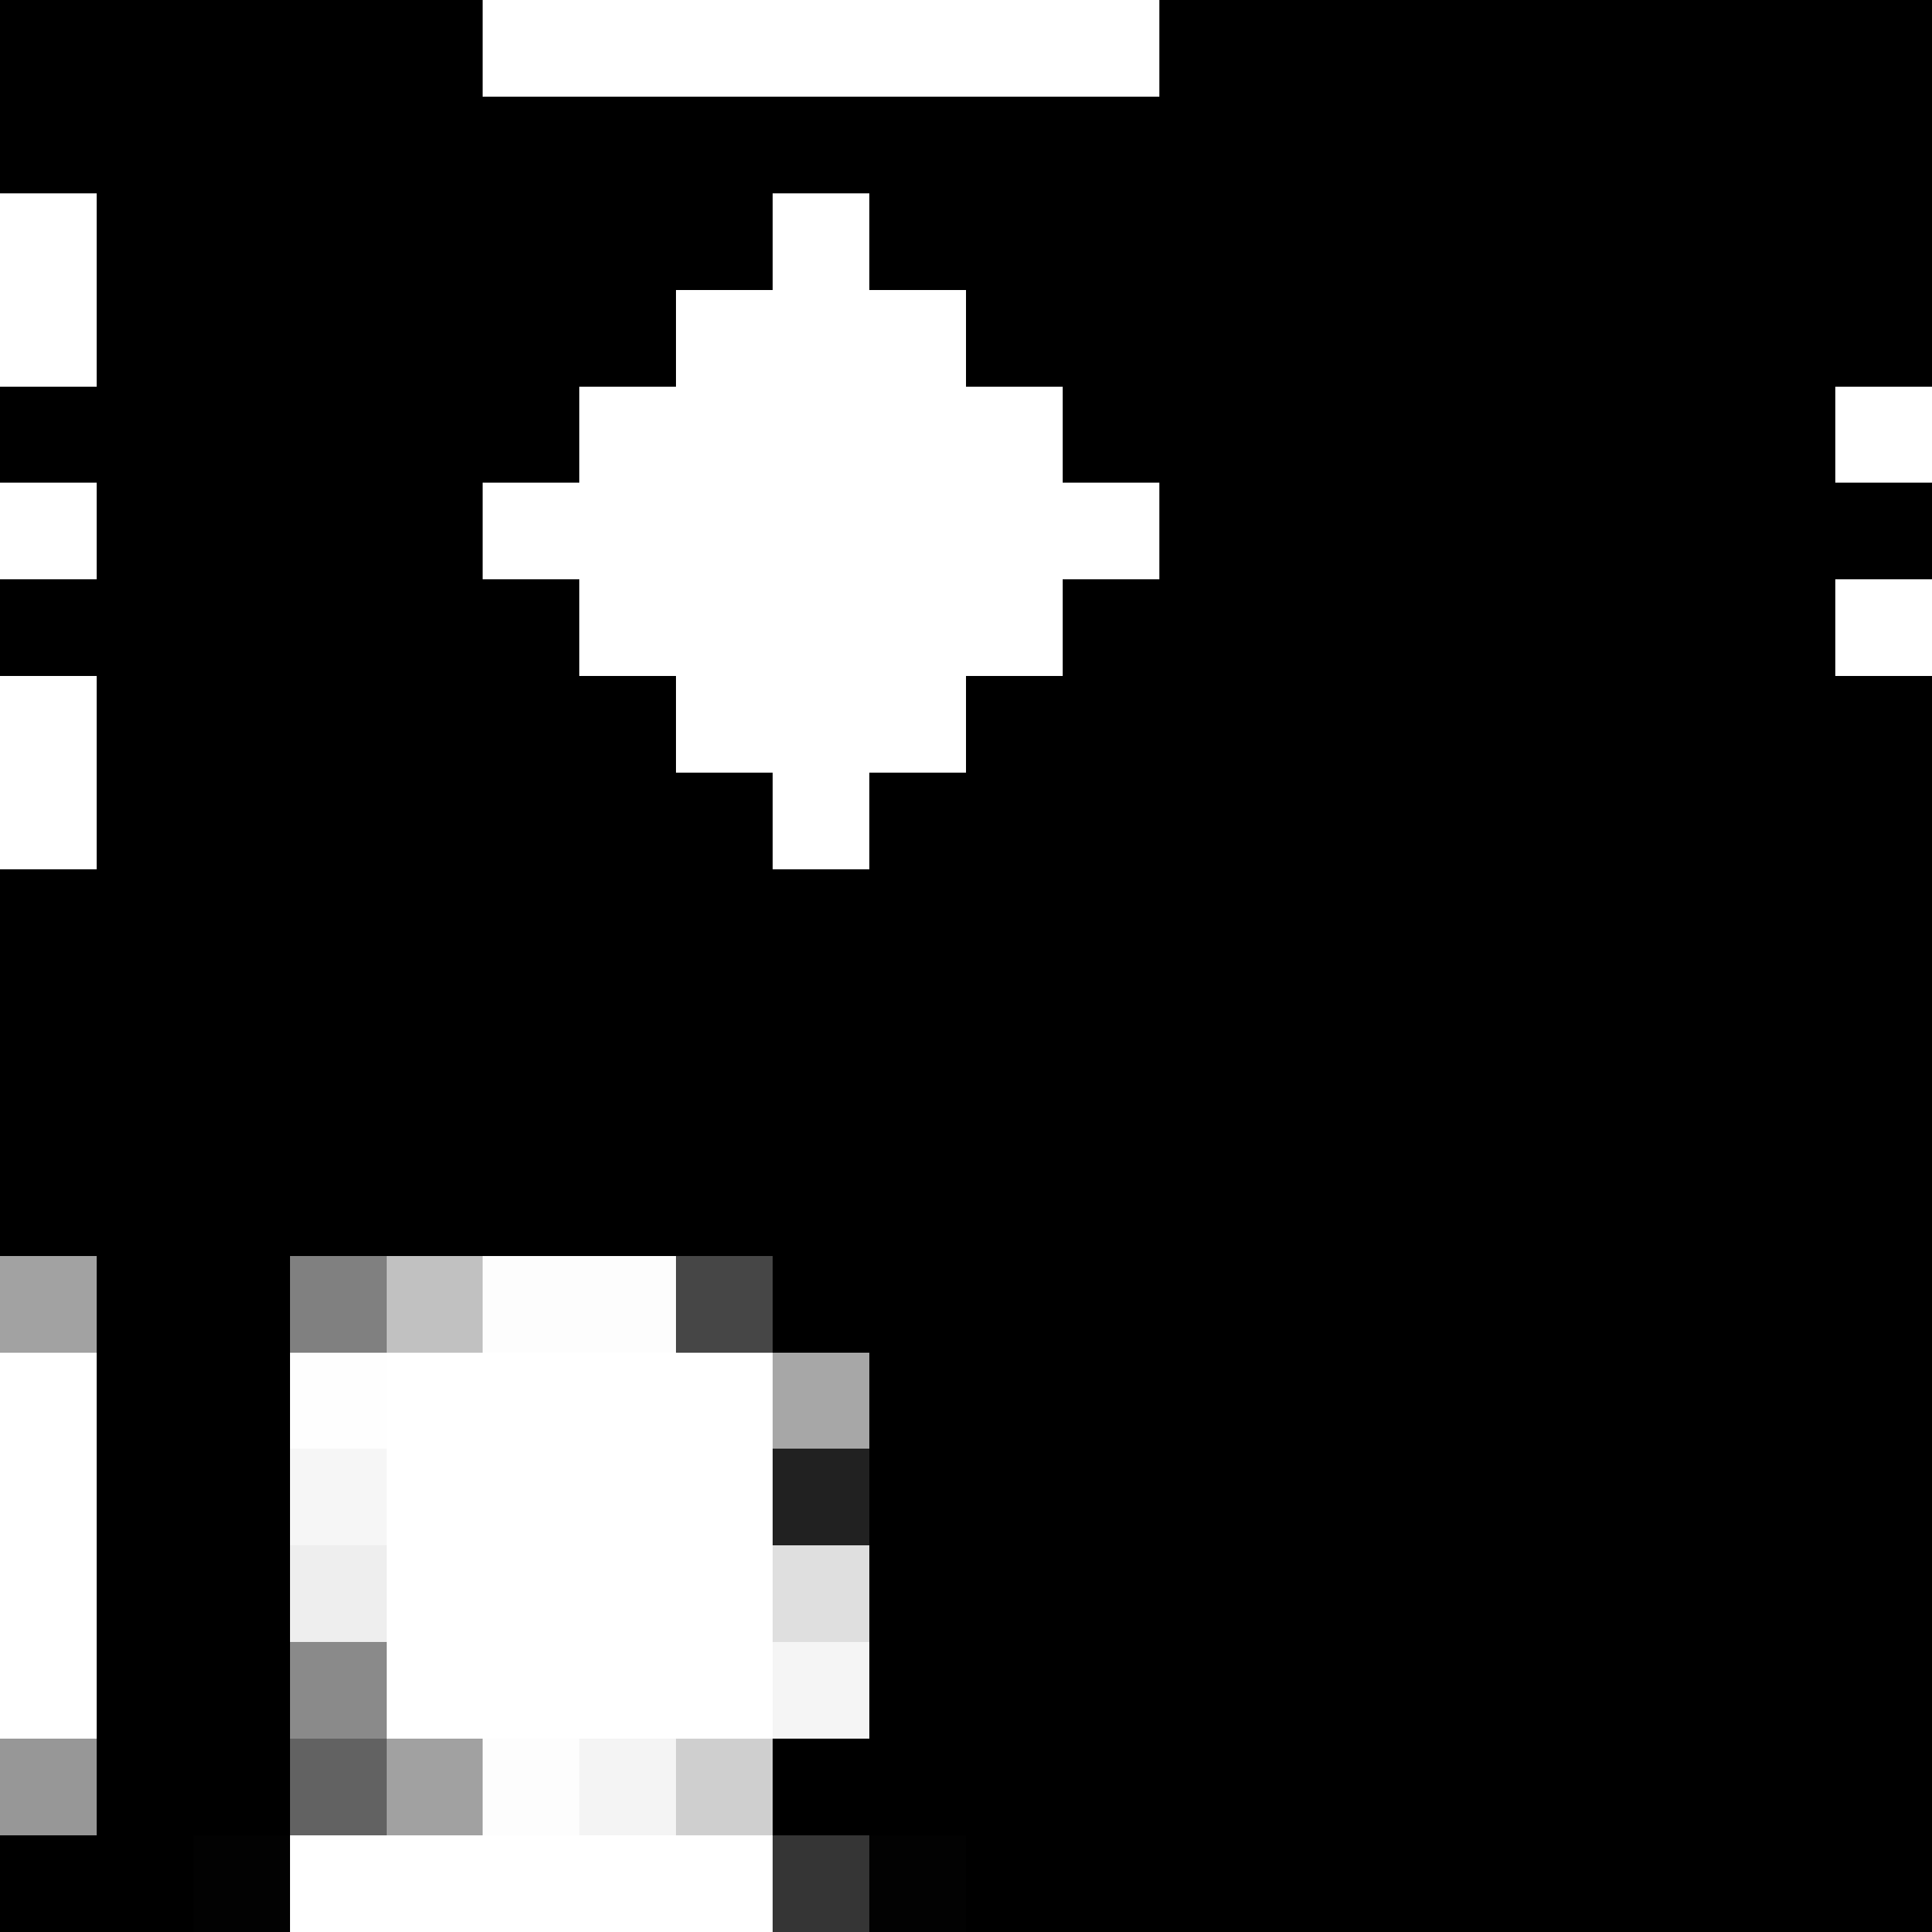
\includegraphics[width=\textwidth]{training_pc_5}
    \end{minipage}
    \begin{minipage}{0.32\textwidth}
        \centering
        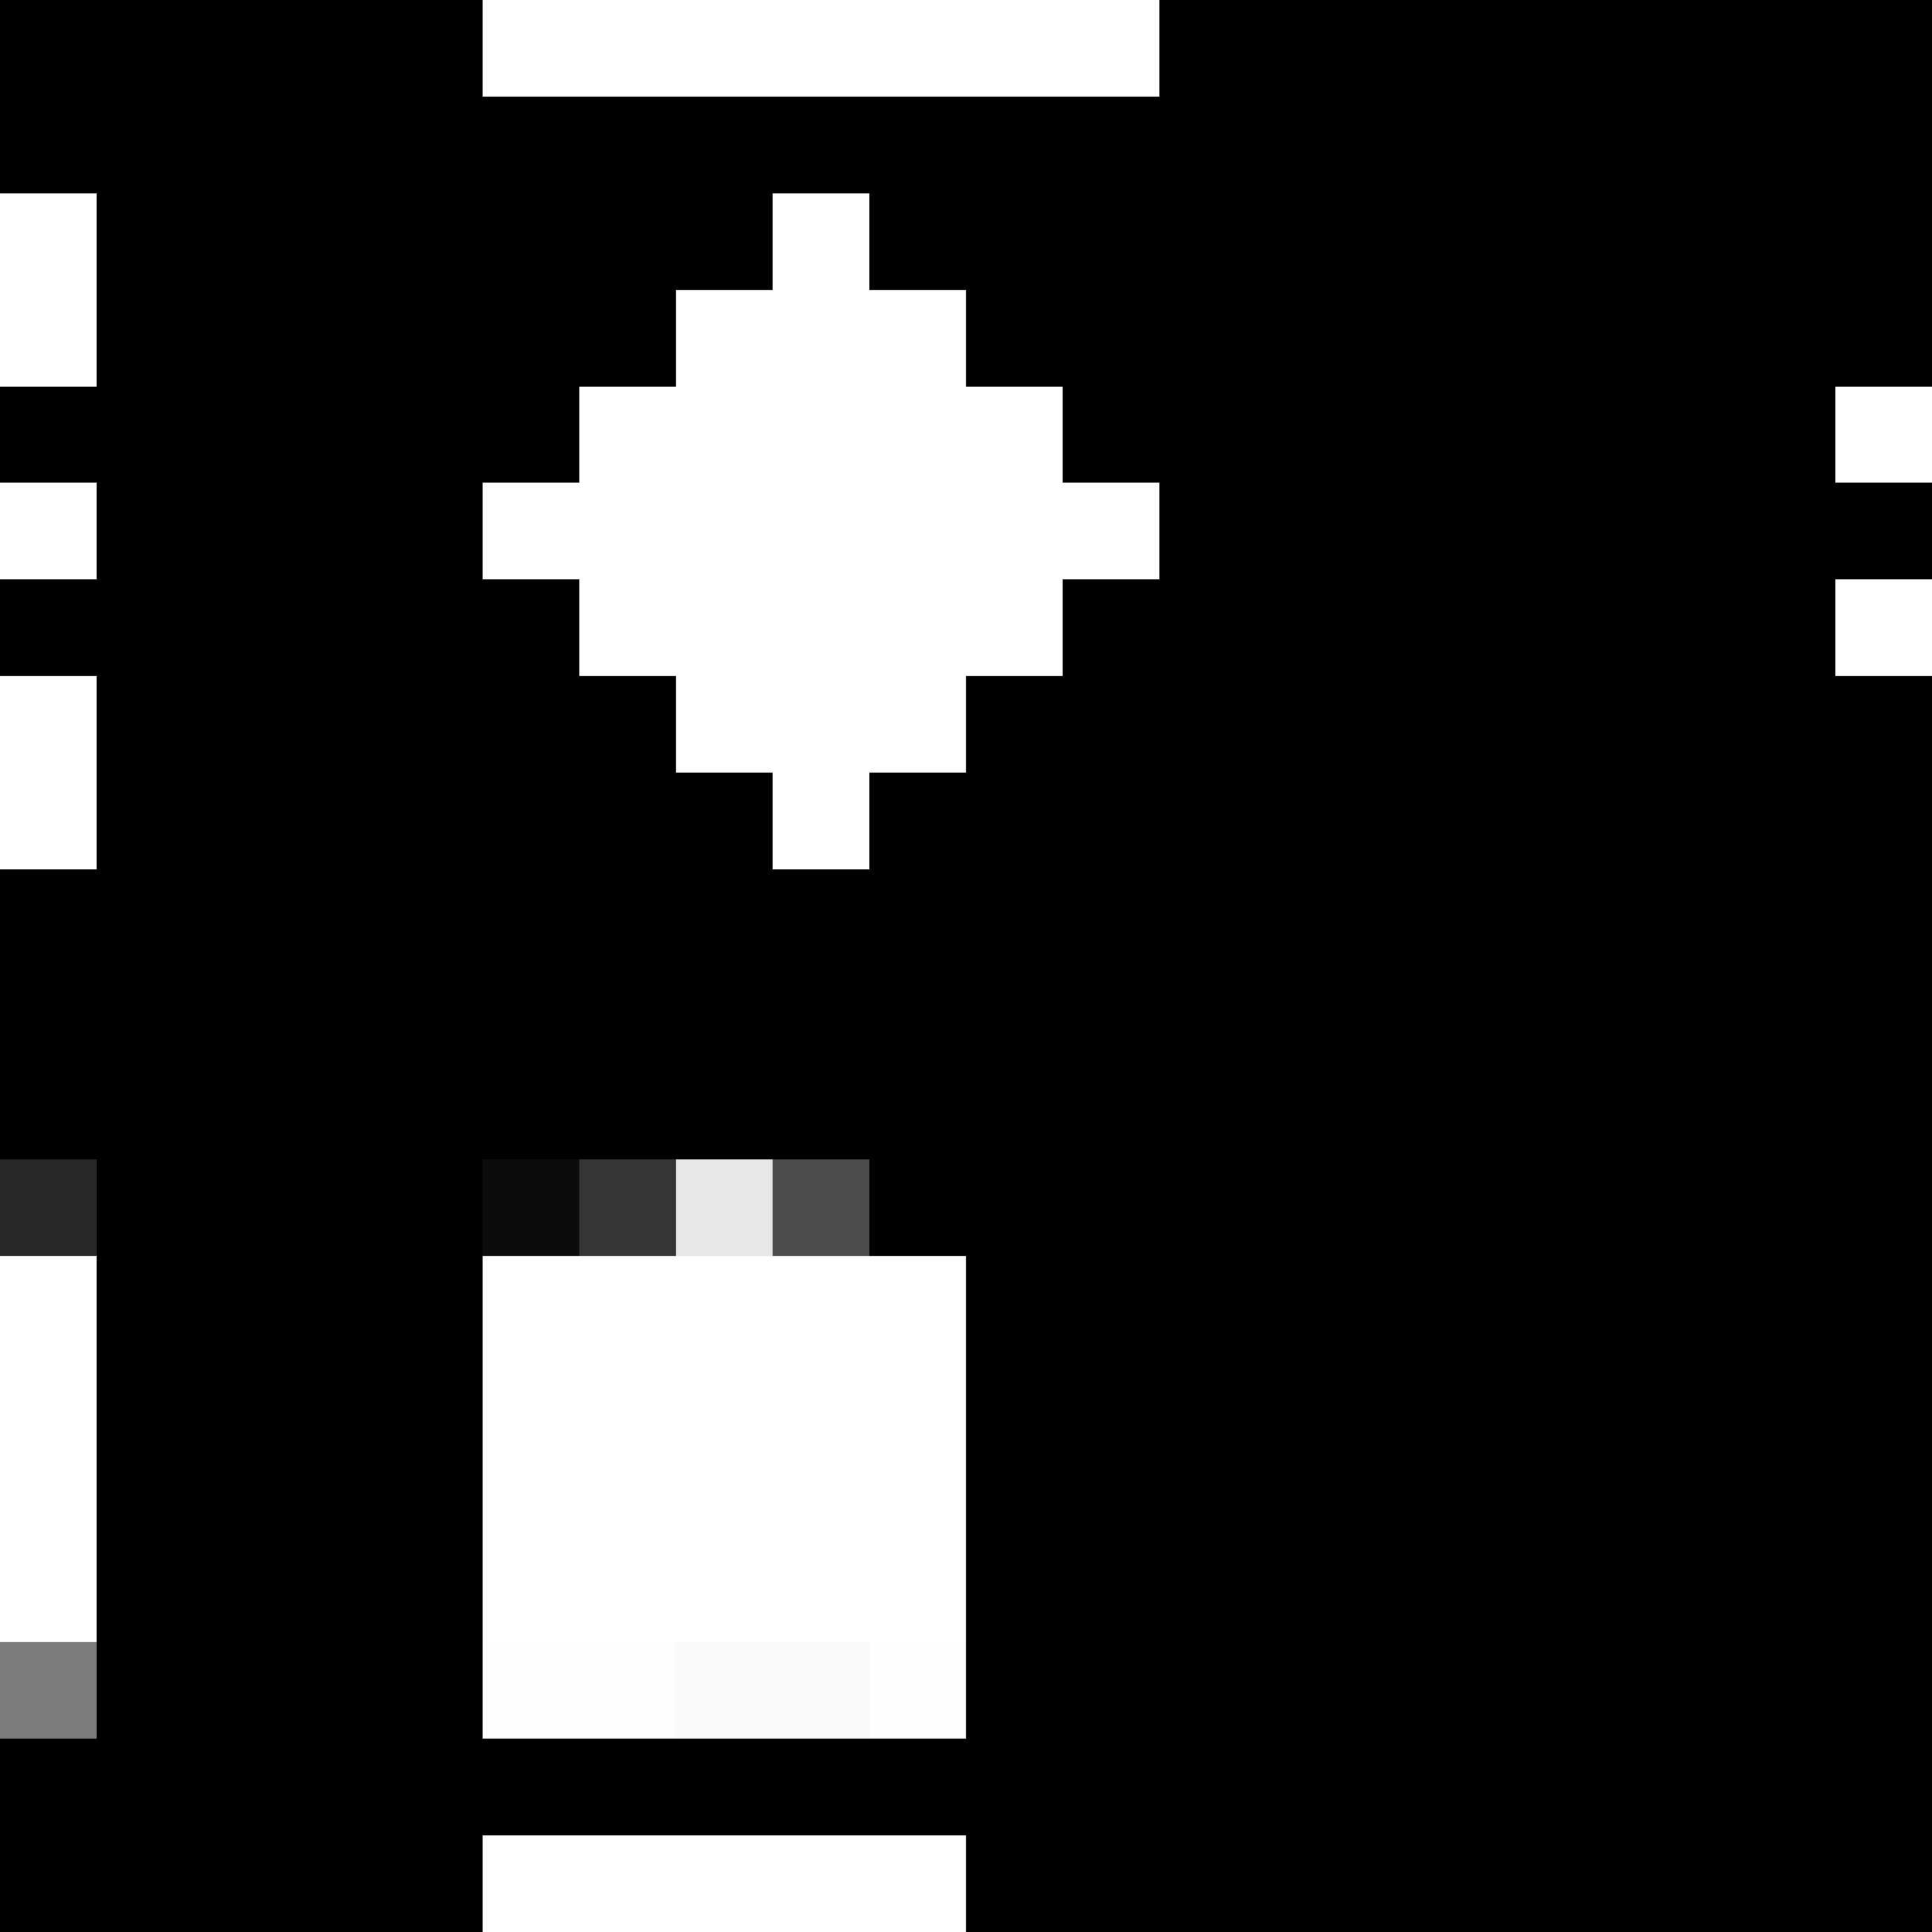
\includegraphics[width=\textwidth]{training_pc_6}
    \end{minipage}
    \caption{Samples drawn at different epochs from the generator trained on \textit{poly20\_pc} (zoom).}
\end{figure}

    \chapter{Conclusions}
\label{ch:conclusions}

The presented results show that constrained adversarial networks enable the encoding of useful prior knowledge in the game theoretic scenario initially proposed by generative adversarial networks. The conducted experiments reveal how constraints on discrete domains can be introduced in the learning procedure to instil knowledge in the deep generative model. The effect is that the proposed architecture is able to approximate the data distribution more closely than its constraints-unaware counterpart of boundary-seeking generative adversarial networks.

Furthermore, by exploring different design choices and analysing several factors, this work offers a number of insights on how these may individually impact on the final performance of the model. For instance, it is observed that the improvement over the baseline seems to increase proportionally with the amount of information conveyed by constraints and becomes particularly relevant when training data is not abundant.

The results also show that the knowledge instillation process is effective even if the information is indirectly provided to the generator via penalty functions computed by the discriminator. Evaluating other design choices for the model is left for future work. Many other architectures, in principle, could provide equivalent or better results. For instance, the original adversarial model may be extended to introduce a third constraints-aware network acting as a regulariser.

Further research is necessary to generalize our results to a wider variety of domains and constraints types. The synthetic data sets used in our experimental setup only allow some preliminary considerations and further testing is required on real-world data. However, the encouraging empirical results indicate a strong potential of constrained adversarial networks to be useful in many other contexts involving constraints beside the obvious one of object generation. For instance, due to its performance in generating new data from input noise, constrained adversarial network could become a building block for larger systems addressing more complex problems, such as optimization, or with specific requirements, such as uniform solution sampling.


%     \chapter*{Acknowledgements} % no numbering

\addcontentsline{toc}{chapter}{Acknowledgements} % add Acknowledgements to TOC

\begin{flushright}
\rightskip=.8cm\textit{``I am a man of fortune and I must seek my fortune''} \\
\vspace{.2em}
\rightskip=.8cm Henry Avery
\end{flushright}
\vspace{1em}


% \textit{Diario di bordo - Giorno 933} % 31/08/2015
% 
% \hfill \break
% Dalla vedetta urlano \textit{``Terra! Terra!''}.\\
% Sembra che anche questa avventura stia volgendo al termine. Tra poco 
% l'\textit{Arca} attraccherà e 
% 
% alzo lo sguardo, incrocio gli occhi dei miei compagni. stanchi e malinconici


% Fai le cose per bene, nello studio e nella vita. La prima parte, quella più facile, l'ho fatta.
% 
% Non capivi cosa facevo. Neanche io. A che serve un PC in mezzo al mare?


% scrollarsi di dosso fardello

% partire per nuove avventure, magari per terra.
% amici della Locanda (bari)

% Amici del leone marino

% Qualche sporadico approdo in isole (Torino)

    
    \addcontentsline{toc}{chapter}{Bibliography} % add bibliography to TOC
    \bibliographystyle{plain} % sort by author name
    \bibliography{12_bibliography}
    
    \appendix
    \chapter{Backpropagation derivation}
\label{sec:appendix_backprop}

The gradient of the loss $l$ with respect to the weight $w_{i,j}$ is computed by using the chain rule:

\begin{equation}
\label{eq:w_gradient}
\frac{\partial l}{\partial w_{i,j}} = \underbrace{\frac{\partial l}{\partial o_j} \cdot \frac{\partial o_j}{\partial net_j}}_\textrm{$\delta_j$} \cdot \frac{\partial net_j}{\partial w_{i,j}}.
\end{equation}

Since the activation function $\varphi$ is differentiable,
\begin{equation}
\label{eq:bp_oj}
\frac{\partial o_j}{\partial net_j} = \frac{\partial \varphi(net_j)}{\partial net_j} = \varphi\prime(net_j).
\end{equation}

By the definition of $net_j$,
\begin{equation}
\label{eq:bp_netj}
\frac{\partial net_j}{\partial w_{i,j}} = \frac{\partial \sum\limits_{k}^{pred_j} w_{k,j} \cdot o_k}{\partial w_{i,j}} = o_i.
\end{equation}

The gradient of the loss $l$ with respect to the output of $h_j$ depends on whether the unit belongs to the final layer or to a hidden layer of the ANN $f$:

\begin{equation}
\label{eq:bp_l}
\frac{\partial l}{\partial o_j} = 
\begin{cases}
     \frac{\partial l}{\partial f(\bm{x}_j)} & \text{if unit $h_j$ in output layer}\\ \\
     \underbrace{\sum\limits_{k}^{succ_j} \frac{\partial l}{\partial o_k} \cdot \frac{\partial o_k}{\partial net_k}}_\textrm{total derivative wrt $o_j$} \cdot w_{j,k} = \sum\limits_{k}^{succ_j} \delta_k \cdot w_{j,k} & \text{otherwise}
\end{cases}.
\end{equation}

Substituting equations \eqref{eq:bp_l}, \eqref{eq:bp_oj} and \eqref{eq:bp_netj} in \eqref{eq:w_gradient} we get:

\begin{equation}
\label{eq:bp_final_new}
\frac{\partial l}{\partial w_{i,j}} = \delta_j \cdot o_i,
\end{equation}

where
\[
\delta_j =
\begin{cases}
     \frac{\partial l}{\partial f(\bm{x}_j)} \cdot \varphi\prime(net_j) & \text{if unit $h_j$ in output layer} \\ \\
     \sum\limits_{k}^{succ_j} \delta_k \cdot w_{j,k} \cdot \varphi\prime(net_j) & \text{otherwise}
\end{cases}.
\]

For example, suppose $\varphi$ is the standard logistic function

\[
\varphi(x) = \frac{1}{1 + e^{-x}} 
\]

with first derivative

\[
\frac{d}{dx}\varphi(x) = \varphi(x)(1 - \varphi(x))
\]

and the loss function $l$ is the Euclidean distance with first derivative

\[
\frac{d}{dx}\varphi(x) = \varphi(x)(1 - \varphi(x)).
\]

The ANN $f$ will first compute an output value $\bm{y} = f(\bm{x})$ and then update every weight according to \eqref{eq:bp_final_new} 

\[
\frac{\partial l}{\partial w_{i,j}} = \delta_j \cdot \bm{y}_i,
\]

where
\[
\delta_j =
\begin{cases}
     (\bm{y}_j - \hat{\bm{y}}_j) \cdot \bm{y}_j \cdot (1 - \bm{y}_j) & \text{if unit $h_j$ in output layer} \\ \\
     (\sum\limits_{k}^{succ_j} \delta_k \cdot w_{j,k}) \cdot \bm{y}_j \cdot (1 - \bm{y}_j) & \text{otherwise}
\end{cases}
\]
and $\hat{\bm{y}}$ is the truth value associated to $\bm{x}$ according to the training set.

    \chapter{Gradient derivation for BGANs}
\label{sec:appendix_bgans}

The goal of BGANs is to train a generator outputting discrete values by estimating gradients for $\bm{\theta}^{(g)}$ via the exclusive Kullback-Leibler divergence between the two joint distributions $\widetilde{p}_{data}(\bm{x}, \bm{z})$ and $p_g(\bm{x}, \bm{z})$:

\begin{equation}
\nabla_{\bm{\theta}^{(g)}} D_{KL}(\widetilde{p}_{data}(\bm{x}, \bm{z}) || p_g(\bm{x}, \bm{z})).
\end{equation}

$\widetilde{p}_{data}(\bm{x}, \bm{z})$ can be assumed to be constant with respect to $\bm{\theta}^{(g)}$ if the one from the previous iteration is used. Thus, $\bm{\theta}^{(g)}$ gradient will not be propagate inside $\widetilde{p}_{data}(\bm{x}, \bm{z})$. Due to \eqref{eq:p_data_estimator} and \eqref{eq:cond_prob_g}, the following holds:

\begin{equation}
\label{eq:joint_estimator}
\widetilde{p}_{data}(\bm{x}, \bm{z}) = \widetilde{p}_{data}(\bm{x}|\bm{z})p(\bm{z}) = \frac{1}{Z_{|\bm{z}}} g(\bm{x}|\bm{z}) \frac{D(\bm{x})}{1-D(\bm{x})} p(\bm{z}),
\end{equation}

where

\[
Z_{|\bm{z}} = \sum_{\bm{x}} g(\bm{x}|\bm{z}) \frac{D(\bm{x})}{1-D(\bm{x})}
\]

and $\widetilde{p}_{data}(\bm{x}|\bm{z})p(\bm{z})$ is an estimate of the data in the neighborhood of the generated samples defined by $\bm{z}$.

The gradient can be estimated as follows:

\begin{align*}
\nabla_{\bm{\theta}^{(g)}} D_{KL}(\widetilde{p}_{data}(\bm{x},\bm{z}) || p_g(\bm{x},\bm{z}))) & = \nabla_{\bm{\theta}^{(g)}} \sum_{\bm{z}} \sum_{\bm{x}} \widetilde{p}_{data}(\bm{x},\bm{z}) \log{\frac{\widetilde{p}_{data}(\bm{x},\bm{z})}{p_g(\bm{x},\bm{z})}} \\
& = \nabla_{\bm{\theta}^{(g)}} \sum_{\bm{z}} \sum_{\bm{x}} \widetilde{p}_{data}(\bm{x},\bm{z}) (\log{\widetilde{p}_{data}(\bm{x},\bm{z}) - \log p_g(\bm{x},\bm{z})}) \\
& = - \sum_{\bm{z}} \sum_{\bm{x}} \widetilde{p}_{data}(\bm{x},\bm{z}) \nabla_{\bm{\theta}^{(g)}} \log p_g(\bm{x},\bm{z}) \\
& \stackrel{\eqref{eq:joint_estimator}}{=} - \sum_{\bm{z}} \sum_{\bm{x}} \frac{1}{Z_{|\bm{z}}}g(\bm{x}|\bm{z})\frac{D(\bm{x})}{1-D(\bm{x})}p(\bm{z}) \nabla_{\bm{\theta}^{(g)}} \log p_g(\bm{x},\bm{z}) \\
& = - \mathbb{E}_{\bm{z} \sim p(\bm{z})} \left[\sum_{\bm{x}} \frac{1}{Z_{|\bm{z}}}\frac{D(\bm{x})}{1-D(\bm{x})}g(\bm{x}|\bm{z}) \nabla_{\bm{\theta}^{(g)}}\log{g(\bm{x}|\bm{z})}\right]\\
& \approx - \mathbb{E}_{\bm{z} \sim p(\bm{z})} \left[\sum\limits_{m = 1}^{M} \frac{1}{M}\frac{1}{Z_{|\bm{z}}}\frac{D(\bm{x}^{(m)})}{1-D(\bm{x}^{(m)})}\nabla_{\bm{\theta}^{(g)}}\log{g(\bm{x}^{(m)}|\bm{z})}\right]
\end{align*}

where we approximated the gradient using $M$ samples
$\bm{x}^{(m)} \sim g(\bm{x}|\bm{z})$ for each $\bm{z}$. Selecting $\bm{x}^{(m)}$ amounts at sampling the discrete values from the probability $g(\bm{x}|\bm{z})$, e.g. a sigmoid function for binary variables.

The samples can also be used to approximate $Z_{|\bm{z}}$ as:
$$
Z_{|\bm{z}} = \sum_{\bm{x}} g(\bm{x}|\bm{z}) \frac{D(\bm{x})}{1-D(\bm{x})} \approx \sum\limits_{m = 1}^{M} \frac{1}{M}\frac{D(\bm{x}^{(m)})}{1-D(\bm{x}^{(m)})}.
$$

For binary variables it is possible to approximate $\nabla_{\bm{\theta}^{(g)}} \log{g(\bm{x}^{(m)}|\bm{z})}$ in the case of a logistic activation function $\sigma$ as follows:

\begin{align*}
\nabla_{\bm{\theta}^{(g)}} \log{g(\bm{x}^{(m)}|\bm{z})}
& = \nabla_{\bm{\theta}^{(g)}} \sum_{i=1}^{|\bm{x}^{(m)}|} \bm{1}_{[\bm{x}_i^{(m)} = 1]} \log{g_i(\bm{x}^{(m)}|\bm{z})} + \bm{1}_{[\bm{x}_i^{(m)} = 0]} \log{(1 - g_i(\bm{x}^{(m)}|\bm{z}))}  \\
& = \nabla_{\bm{\theta}^{(g)}} \sum_{i=1}^{|\bm{x}^{(m)}|} \bm{1}_{[\bm{x}_i^{(m)} = 1]} \log{\sigma(h_i(\bm{x}^{(m)}|\bm{z}))} + \bm{1}_{[\bm{x}_i^{(m)} = 0]} \log{(1 - \sigma(h_i(\bm{x}^{(m)}|\bm{z})))} \\
& =  \nabla_{\bm{\theta}^{(g)}} \sum_{i=1}^{|\bm{x}^{(m)}|} \bm{1}_{[\bm{x}_i^{(m)} = 1]} \log{\frac{1}{1+e^{-h_i(\bm{x}^{(m)}|\bm{z})}}}+ \bm{1}_{[\bm{x}_i^{(m)} = 0]} \log{\frac{e^{-h_i(\bm{x}^{(m)}|\bm{z})}}{1+e^{-h_i(\bm{x}^{(m)}|\bm{z})}}} \\                                
& =  - \nabla_{\bm{\theta}^{(g)}} \sum_{i=1}^{|\bm{x}^{(m)}|}\log{(1+e^{-h_i(\bm{x}^{(m)}|\bm{z})})} + \bm{1}_{[\bm{x}_i^{(m)} = 0]}h_i(\bm{x}^{(m)}|\bm{z}) \\
& \approx  - \nabla_{\bm{\theta}^{(g)}} \sum_{i=1}^{|\bm{x}^{(m)}|}\max{(0,-h_i(\bm{x}^{(m)}|\bm{z}))} + \bm{1}_{[\bm{x}_i^{(m)} = 0]}h_i(\bm{x}^{(m)}|\bm{z}),
\end{align*}

since $\log{(1+e^{-\bm{x}})} \approx \max{(0,-\bm{x})}$.


\end{document}


% TODO
% - prune useless notation
% - full text in Eng
% - Acknow
